\documentclass[11pt]{article}
\usepackage[margin=1in]{geometry}
\usepackage{amsmath,amssymb}
\usepackage{graphicx}
\usepackage{booktabs}
\usepackage[hyphens]{url}
\usepackage[colorlinks=true,linkcolor=blue,citecolor=blue,urlcolor=blue]{hyperref}
\usepackage{parskip}
\usepackage{enumitem}
\usepackage{tikz}
\usetikzlibrary{positioning}
% The flow diagram: its lengths are set here, and its counts are \num{...} like every other number.
\newlength{\flowwidth}\setlength{\flowwidth}{4.5cm}
\newlength{\flowgap}\setlength{\flowgap}{6mm}
\tikzset{
  flowpic/.style={node distance=\flowgap and \flowgap, >=latex},
  flow/.style={draw, rounded corners=1pt, align=flush center, font=\footnotesize, inner sep=4pt, text width=\flowwidth, minimum height=1cm},
  flowwide/.style={flow, text width=\dimexpr 2\flowwidth+\flowgap+8pt\relax},
  flowaside/.style={flow, dashed},
}
\usepackage{xr}
\externaldocument{supplement}
\graphicspath{{./}}
% a float gets a page of its own only if it fills most of it; a smaller one goes to the top of a page of text (the default of 0.5 leaves half-empty pages)
\renewcommand{\floatpagefraction}{0.65}
% let TeX stretch a line rather than push unbreakable code names into the margin
\emergencystretch=3em
% never break a line or a page inside inline math, so that "p =" keeps its value
\relpenalty=10000
\binoppenalty=10000

% Every number in this paper is written by the analysis scripts: numbers.tex defines \num{name}.
% Generated by write_numbers.py from numbers/*.json. Do not edit.
\makeatletter
\newcommand{\num}[1]{%
  \@ifundefined{num@#1}{\errmessage{Unknown number: #1}}{\@nameuse{num@#1}}}
% rows of a generated table; the primitive \input works inside a tabular
\newcommand{\tablebody}[1]{\@@input tables/#1.tex }
\@namedef{num@allYears.last}{2026}
\@namedef{num@alpha}{0.05}
\@namedef{num@analyses.absent}{1}
\@namedef{num@analyses.absent.withVerdict}{0}
\@namedef{num@analyses.notInCohort}{82}
\@namedef{num@area.Cardiometabolic.miss.n}{48}
\@namedef{num@area.Cardiometabolic.miss.pct}{20.9}
\@namedef{num@area.Cardiometabolic.miss.pct.int}{21}
\@namedef{num@area.Cardiometabolic.trials}{230}
\@namedef{num@area.ImmunologyInflammation.miss.n}{56}
\@namedef{num@area.ImmunologyInflammation.miss.pct}{17.4}
\@namedef{num@area.ImmunologyInflammation.miss.pct.int}{17}
\@namedef{num@area.ImmunologyInflammation.trials}{322}
\@namedef{num@area.InfectiousVaccine.miss.n}{82}
\@namedef{num@area.InfectiousVaccine.miss.pct}{43.2}
\@namedef{num@area.InfectiousVaccine.miss.pct.int}{43}
\@namedef{num@area.InfectiousVaccine.trials}{190}
\@namedef{num@area.NeuroPsych.miss.n}{82}
\@namedef{num@area.NeuroPsych.miss.pct}{36.1}
\@namedef{num@area.NeuroPsych.miss.pct.int}{36}
\@namedef{num@area.NeuroPsych.trials}{227}
\@namedef{num@area.Oncology.miss.n}{119}
\@namedef{num@area.Oncology.miss.pct}{36.1}
\@namedef{num@area.Oncology.miss.pct.int}{36}
\@namedef{num@area.Oncology.trials}{330}
\@namedef{num@area.Otherrare.miss.n}{163}
\@namedef{num@area.Otherrare.miss.pct}{32.3}
\@namedef{num@area.Otherrare.miss.pct.int}{32}
\@namedef{num@area.Otherrare.trials}{505}
\@namedef{num@area.het.chi2}{59.5}
\@namedef{num@area.het.dof}{5}
\@namedef{num@area.het.p}{2\times10^{-11}}
\@namedef{num@area.infectious.before.miss.n}{17}
\@namedef{num@area.infectious.before.miss.pct}{28.8}
\@namedef{num@area.infectious.before.miss.pct.int}{29}
\@namedef{num@area.infectious.before.trials}{59}
\@namedef{num@area.infectious.from.miss.n}{65}
\@namedef{num@area.infectious.from.miss.pct}{49.6}
\@namedef{num@area.infectious.from.miss.pct.int}{50}
\@namedef{num@area.infectious.from.trials}{131}
\@namedef{num@area.infectious.p}{0.0074}
\@namedef{num@area.infectious.split}{2020}
\@namedef{num@area.infectious.z}{2.7}
\@namedef{num@audit.eff.interim}{2}
\@namedef{num@audit.eff.monitoring}{7}
\@namedef{num@audit.eff.n}{10}
\@namedef{num@audit.eff.ncts}{NCT03847090, NCT03988023, NCT04084678, NCT04539275, NCT04581915, NCT04901676, NCT04901689, NCT05008926, NCT05288855, NCT05962788}
\@namedef{num@audit.eff.other}{1}
\@namedef{num@audit.model.n}{25}
\@namedef{num@bigpharma.companies}{17}
\@namedef{num@bigpharma.mid}{18}
\@namedef{num@bigpharma.patterns}{93}
\@namedef{num@bigpharma.sponsorNames}{144}
\@namedef{num@bigpharma.wide.sponsorNames}{232}
\@namedef{num@classification.month}{July 2026}
\@namedef{num@cohort.analysed}{17{,}054}
\@namedef{num@cohort.both}{1{,}854}
\@namedef{num@cohort.era.stopped}{2{,}023}
\@namedef{num@cohort.era.withdrawn.n}{652}
\@namedef{num@cohort.era.withdrawn.pct}{32.2}
\@namedef{num@cohort.era.withdrawn.pct.int}{32}
\@namedef{num@cohort.noDrug.n}{1{,}253}
\@namedef{num@cohort.noDrug.pct}{6.8}
\@namedef{num@cohort.noDrug.pct.int}{7}
\@namedef{num@cohort.noStartYear}{113}
\@namedef{num@cohort.results}{14{,}633}
\@namedef{num@cohort.results.completed}{12{,}430}
\@namedef{num@cohort.results.other}{351}
\@namedef{num@cohort.results.terminated}{1{,}852}
\@namedef{num@cohort.sponsorNames}{3{,}170}
\@namedef{num@cohort.startAfterWindow}{3}
\@namedef{num@cohort.stopped}{5{,}687}
\@namedef{num@cohort.stoppedEnrolled}{4{,}275}
\@namedef{num@cohort.suspended}{152}
\@namedef{num@cohort.terminated}{4{,}123}
\@namedef{num@cohort.unique}{18{,}466}
\@namedef{num@cohort.withdrawn}{1{,}412}
\@namedef{num@combine.all.and.n}{2{,}432}
\@namedef{num@combine.all.and.pct}{36.9}
\@namedef{num@combine.all.and.pct.int}{37}
\@namedef{num@combine.all.any.n}{2{,}079}
\@namedef{num@combine.all.any.pct}{31.5}
\@namedef{num@combine.all.any.pct.int}{32}
\@namedef{num@combine.all.incomplete.n}{756}
\@namedef{num@combine.all.incomplete.pct}{11.5}
\@namedef{num@combine.all.incomplete.pct.int}{11}
\@namedef{num@combine.all.strict.n}{2{,}906}
\@namedef{num@combine.all.strict.pct}{44.0}
\@namedef{num@combine.all.strict.pct.int}{44}
\@namedef{num@combine.all.trials}{6{,}598}
\@namedef{num@combine.era.and.n}{643}
\@namedef{num@combine.era.and.pct}{35.6}
\@namedef{num@combine.era.and.pct.int}{36}
\@namedef{num@combine.era.any.n}{550}
\@namedef{num@combine.era.any.pct}{30.5}
\@namedef{num@combine.era.any.pct.int}{30}
\@namedef{num@combine.era.incomplete.n}{218}
\@namedef{num@combine.era.incomplete.pct}{12.1}
\@namedef{num@combine.era.incomplete.pct.int}{12}
\@namedef{num@combine.era.strict.n}{778}
\@namedef{num@combine.era.strict.pct}{43.1}
\@namedef{num@combine.era.strict.pct.int}{43}
\@namedef{num@combine.era.trials}{1{,}804}
\@namedef{num@coverage.enrolled.all.adjusted.com}{18.7}
\@namedef{num@coverage.enrolled.all.adjusted.com.int}{19}
\@namedef{num@coverage.enrolled.all.adjusted.eff}{47.8}
\@namedef{num@coverage.enrolled.all.adjusted.eff.int}{48}
\@namedef{num@coverage.enrolled.all.adjusted.extra}{351}
\@namedef{num@coverage.enrolled.all.adjusted.op}{30.3}
\@namedef{num@coverage.enrolled.all.adjusted.op.int}{30}
\@namedef{num@coverage.enrolled.all.adjusted.saf}{2.1}
\@namedef{num@coverage.enrolled.all.adjusted.saf.int}{2}
\@namedef{num@coverage.enrolled.all.adjusted.unk}{1.2}
\@namedef{num@coverage.enrolled.all.adjusted.unk.int}{1}
\@namedef{num@coverage.enrolled.all.all.miss.n}{382}
\@namedef{num@coverage.enrolled.all.all.miss.pct}{26.9}
\@namedef{num@coverage.enrolled.all.all.miss.pct.int}{27}
\@namedef{num@coverage.enrolled.all.comparator.coverage.pct}{54.5}
\@namedef{num@coverage.enrolled.all.comparator.coverage.pct.int}{55}
\@namedef{num@coverage.enrolled.all.comparator.miss.n}{376}
\@namedef{num@coverage.enrolled.all.comparator.miss.pct}{27.3}
\@namedef{num@coverage.enrolled.all.comparator.miss.pct.int}{27}
\@namedef{num@coverage.enrolled.all.comparator.noArmGroups}{1}
\@namedef{num@coverage.enrolled.all.comparator.reported}{1{,}379}
\@namedef{num@coverage.enrolled.all.comparator.unreported}{1{,}151}
\@namedef{num@coverage.enrolled.all.completed}{3{,}002}
\@namedef{num@coverage.enrolled.all.pooled.com}{19.0}
\@namedef{num@coverage.enrolled.all.pooled.com.int}{19}
\@namedef{num@coverage.enrolled.all.pooled.eff}{46.8}
\@namedef{num@coverage.enrolled.all.pooled.eff.hi}{47.5}
\@namedef{num@coverage.enrolled.all.pooled.eff.hi.int}{48}
\@namedef{num@coverage.enrolled.all.pooled.eff.int}{47}
\@namedef{num@coverage.enrolled.all.pooled.eff.lo}{46.1}
\@namedef{num@coverage.enrolled.all.pooled.eff.lo.int}{46}
\@namedef{num@coverage.enrolled.all.pooled.extra}{314}
\@namedef{num@coverage.enrolled.all.pooled.op}{30.9}
\@namedef{num@coverage.enrolled.all.pooled.op.hi}{31.3}
\@namedef{num@coverage.enrolled.all.pooled.op.hi.int}{31}
\@namedef{num@coverage.enrolled.all.pooled.op.int}{31}
\@namedef{num@coverage.enrolled.all.pooled.op.lo}{30.5}
\@namedef{num@coverage.enrolled.all.pooled.op.lo.int}{30}
\@namedef{num@coverage.enrolled.all.pooled.saf}{2.1}
\@namedef{num@coverage.enrolled.all.pooled.saf.int}{2}
\@namedef{num@coverage.enrolled.all.pooled.unk}{1.2}
\@namedef{num@coverage.enrolled.all.pooled.unk.int}{1}
\@namedef{num@coverage.enrolled.all.raw.com}{22.5}
\@namedef{num@coverage.enrolled.all.raw.com.int}{22}
\@namedef{num@coverage.enrolled.all.raw.eff}{37.1}
\@namedef{num@coverage.enrolled.all.raw.eff.int}{37}
\@namedef{num@coverage.enrolled.all.raw.extra}{0}
\@namedef{num@coverage.enrolled.all.raw.op}{36.5}
\@namedef{num@coverage.enrolled.all.raw.op.int}{37}
\@namedef{num@coverage.enrolled.all.raw.saf}{2.5}
\@namedef{num@coverage.enrolled.all.raw.saf.int}{2}
\@namedef{num@coverage.enrolled.all.raw.unk}{1.4}
\@namedef{num@coverage.enrolled.all.raw.unk.int}{1}
\@namedef{num@coverage.enrolled.all.reported.n}{1{,}419}
\@namedef{num@coverage.enrolled.all.reported.pct}{47.3}
\@namedef{num@coverage.enrolled.all.reported.pct.int}{47}
\@namedef{num@coverage.enrolled.all.singleArm.reported.n}{40}
\@namedef{num@coverage.enrolled.all.singleArm.reported.pct}{2.8}
\@namedef{num@coverage.enrolled.all.singleArm.reported.pct.int}{3}
\@namedef{num@coverage.enrolled.all.singleArm.unreported.n}{432}
\@namedef{num@coverage.enrolled.all.singleArm.unreported.pct}{27.3}
\@namedef{num@coverage.enrolled.all.singleArm.unreported.pct.int}{27}
\@namedef{num@coverage.enrolled.all.unreported.n}{1{,}583}
\@namedef{num@coverage.enrolled.all.unreported.pct}{52.7}
\@namedef{num@coverage.enrolled.all.unreported.pct.int}{53}
\@namedef{num@coverage.enrolled.all.upper.com}{13.5}
\@namedef{num@coverage.enrolled.all.upper.com.int}{13}
\@namedef{num@coverage.enrolled.all.upper.eff}{62.3}
\@namedef{num@coverage.enrolled.all.upper.eff.int}{62}
\@namedef{num@coverage.enrolled.all.upper.extra}{1{,}151}
\@namedef{num@coverage.enrolled.all.upper.op}{21.9}
\@namedef{num@coverage.enrolled.all.upper.op.int}{22}
\@namedef{num@coverage.enrolled.all.upper.saf}{1.5}
\@namedef{num@coverage.enrolled.all.upper.saf.int}{1}
\@namedef{num@coverage.enrolled.all.upper.unk}{0.8}
\@namedef{num@coverage.enrolled.all.upper.unk.int}{1}
\@namedef{num@coverage.enrolled.all.withSingleArm.com}{18.0}
\@namedef{num@coverage.enrolled.all.withSingleArm.com.int}{18}
\@namedef{num@coverage.enrolled.all.withSingleArm.eff}{49.6}
\@namedef{num@coverage.enrolled.all.withSingleArm.eff.int}{50}
\@namedef{num@coverage.enrolled.all.withSingleArm.extra}{426}
\@namedef{num@coverage.enrolled.all.withSingleArm.op}{29.3}
\@namedef{num@coverage.enrolled.all.withSingleArm.op.int}{29}
\@namedef{num@coverage.enrolled.all.withSingleArm.saf}{2.0}
\@namedef{num@coverage.enrolled.all.withSingleArm.saf.int}{2}
\@namedef{num@coverage.enrolled.all.withSingleArm.unk}{1.1}
\@namedef{num@coverage.enrolled.all.withSingleArm.unk.int}{1}
\@namedef{num@coverage.enrolled.big.adjusted.com}{23.4}
\@namedef{num@coverage.enrolled.big.adjusted.com.int}{23}
\@namedef{num@coverage.enrolled.big.adjusted.eff}{60.5}
\@namedef{num@coverage.enrolled.big.adjusted.eff.int}{60}
\@namedef{num@coverage.enrolled.big.adjusted.extra}{66}
\@namedef{num@coverage.enrolled.big.adjusted.op}{12.1}
\@namedef{num@coverage.enrolled.big.adjusted.op.int}{12}
\@namedef{num@coverage.enrolled.big.adjusted.saf}{2.7}
\@namedef{num@coverage.enrolled.big.adjusted.saf.int}{3}
\@namedef{num@coverage.enrolled.big.adjusted.unk}{1.3}
\@namedef{num@coverage.enrolled.big.adjusted.unk.int}{1}
\@namedef{num@coverage.enrolled.big.all.miss.n}{138}
\@namedef{num@coverage.enrolled.big.all.miss.pct}{22.0}
\@namedef{num@coverage.enrolled.big.all.miss.pct.int}{22}
\@namedef{num@coverage.enrolled.big.comparator.coverage.pct}{67.0}
\@namedef{num@coverage.enrolled.big.comparator.coverage.pct.int}{67}
\@namedef{num@coverage.enrolled.big.comparator.miss.n}{138}
\@namedef{num@coverage.enrolled.big.comparator.miss.pct}{22.6}
\@namedef{num@coverage.enrolled.big.comparator.miss.pct.int}{23}
\@namedef{num@coverage.enrolled.big.comparator.noArmGroups}{0}
\@namedef{num@coverage.enrolled.big.comparator.reported}{611}
\@namedef{num@coverage.enrolled.big.comparator.unreported}{301}
\@namedef{num@coverage.enrolled.big.completed}{1{,}112}
\@namedef{num@coverage.enrolled.big.pooled.com}{23.3}
\@namedef{num@coverage.enrolled.big.pooled.com.int}{23}
\@namedef{num@coverage.enrolled.big.pooled.eff}{60.7}
\@namedef{num@coverage.enrolled.big.pooled.eff.hi}{61.5}
\@namedef{num@coverage.enrolled.big.pooled.eff.hi.int}{62}
\@namedef{num@coverage.enrolled.big.pooled.eff.int}{61}
\@namedef{num@coverage.enrolled.big.pooled.eff.lo}{59.8}
\@namedef{num@coverage.enrolled.big.pooled.eff.lo.int}{60}
\@namedef{num@coverage.enrolled.big.pooled.extra}{68}
\@namedef{num@coverage.enrolled.big.pooled.op}{12.0}
\@namedef{num@coverage.enrolled.big.pooled.op.hi}{12.3}
\@namedef{num@coverage.enrolled.big.pooled.op.hi.int}{12}
\@namedef{num@coverage.enrolled.big.pooled.op.int}{12}
\@namedef{num@coverage.enrolled.big.pooled.op.lo}{11.7}
\@namedef{num@coverage.enrolled.big.pooled.op.lo.int}{12}
\@namedef{num@coverage.enrolled.big.pooled.saf}{2.7}
\@namedef{num@coverage.enrolled.big.pooled.saf.int}{3}
\@namedef{num@coverage.enrolled.big.pooled.unk}{1.3}
\@namedef{num@coverage.enrolled.big.pooled.unk.int}{1}
\@namedef{num@coverage.enrolled.big.raw.com}{27.5}
\@namedef{num@coverage.enrolled.big.raw.com.int}{27}
\@namedef{num@coverage.enrolled.big.raw.eff}{53.7}
\@namedef{num@coverage.enrolled.big.raw.eff.int}{54}
\@namedef{num@coverage.enrolled.big.raw.extra}{0}
\@namedef{num@coverage.enrolled.big.raw.op}{14.1}
\@namedef{num@coverage.enrolled.big.raw.op.int}{14}
\@namedef{num@coverage.enrolled.big.raw.saf}{3.1}
\@namedef{num@coverage.enrolled.big.raw.saf.int}{3}
\@namedef{num@coverage.enrolled.big.raw.unk}{1.6}
\@namedef{num@coverage.enrolled.big.raw.unk.int}{2}
\@namedef{num@coverage.enrolled.big.reported.n}{627}
\@namedef{num@coverage.enrolled.big.reported.pct}{56.4}
\@namedef{num@coverage.enrolled.big.reported.pct.int}{56}
\@namedef{num@coverage.enrolled.big.singleArm.reported.n}{16}
\@namedef{num@coverage.enrolled.big.singleArm.reported.pct}{2.6}
\@namedef{num@coverage.enrolled.big.singleArm.reported.pct.int}{3}
\@namedef{num@coverage.enrolled.big.singleArm.unreported.n}{184}
\@namedef{num@coverage.enrolled.big.singleArm.unreported.pct}{37.9}
\@namedef{num@coverage.enrolled.big.singleArm.unreported.pct.int}{38}
\@namedef{num@coverage.enrolled.big.unreported.n}{485}
\@namedef{num@coverage.enrolled.big.unreported.pct}{43.6}
\@namedef{num@coverage.enrolled.big.unreported.pct.int}{44}
\@namedef{num@coverage.enrolled.big.upper.com}{15.4}
\@namedef{num@coverage.enrolled.big.upper.com.int}{15}
\@namedef{num@coverage.enrolled.big.upper.eff}{74.1}
\@namedef{num@coverage.enrolled.big.upper.eff.int}{74}
\@namedef{num@coverage.enrolled.big.upper.extra}{301}
\@namedef{num@coverage.enrolled.big.upper.op}{7.9}
\@namedef{num@coverage.enrolled.big.upper.op.int}{8}
\@namedef{num@coverage.enrolled.big.upper.saf}{1.8}
\@namedef{num@coverage.enrolled.big.upper.saf.int}{2}
\@namedef{num@coverage.enrolled.big.upper.unk}{0.9}
\@namedef{num@coverage.enrolled.big.upper.unk.int}{1}
\@namedef{num@coverage.enrolled.big.withSingleArm.com}{21.5}
\@namedef{num@coverage.enrolled.big.withSingleArm.com.int}{21}
\@namedef{num@coverage.enrolled.big.withSingleArm.eff}{63.8}
\@namedef{num@coverage.enrolled.big.withSingleArm.eff.int}{64}
\@namedef{num@coverage.enrolled.big.withSingleArm.extra}{107}
\@namedef{num@coverage.enrolled.big.withSingleArm.op}{11.0}
\@namedef{num@coverage.enrolled.big.withSingleArm.op.int}{11}
\@namedef{num@coverage.enrolled.big.withSingleArm.saf}{2.5}
\@namedef{num@coverage.enrolled.big.withSingleArm.saf.int}{2}
\@namedef{num@coverage.enrolled.big.withSingleArm.unk}{1.2}
\@namedef{num@coverage.enrolled.big.withSingleArm.unk.int}{1}
\@namedef{num@coverage.enrolled.rest.adjusted.com}{17.4}
\@namedef{num@coverage.enrolled.rest.adjusted.com.int}{17}
\@namedef{num@coverage.enrolled.rest.adjusted.eff}{44.2}
\@namedef{num@coverage.enrolled.rest.adjusted.eff.int}{44}
\@namedef{num@coverage.enrolled.rest.adjusted.extra}{282}
\@namedef{num@coverage.enrolled.rest.adjusted.op}{35.4}
\@namedef{num@coverage.enrolled.rest.adjusted.op.int}{35}
\@namedef{num@coverage.enrolled.rest.adjusted.saf}{1.9}
\@namedef{num@coverage.enrolled.rest.adjusted.saf.int}{2}
\@namedef{num@coverage.enrolled.rest.adjusted.unk}{1.1}
\@namedef{num@coverage.enrolled.rest.adjusted.unk.int}{1}
\@namedef{num@coverage.enrolled.rest.all.miss.n}{244}
\@namedef{num@coverage.enrolled.rest.all.miss.pct}{30.8}
\@namedef{num@coverage.enrolled.rest.all.miss.pct.int}{31}
\@namedef{num@coverage.enrolled.rest.comparator.coverage.pct}{47.5}
\@namedef{num@coverage.enrolled.rest.comparator.coverage.pct.int}{47}
\@namedef{num@coverage.enrolled.rest.comparator.miss.n}{238}
\@namedef{num@coverage.enrolled.rest.comparator.miss.pct}{31.0}
\@namedef{num@coverage.enrolled.rest.comparator.miss.pct.int}{31}
\@namedef{num@coverage.enrolled.rest.comparator.noArmGroups}{1}
\@namedef{num@coverage.enrolled.rest.comparator.reported}{768}
\@namedef{num@coverage.enrolled.rest.comparator.unreported}{850}
\@namedef{num@coverage.enrolled.rest.completed}{1{,}890}
\@namedef{num@coverage.enrolled.rest.needed.n}{140}
\@namedef{num@coverage.enrolled.rest.needed.pct}{16.5}
\@namedef{num@coverage.enrolled.rest.needed.pct.int}{16}
\@namedef{num@coverage.enrolled.rest.pooled.com}{17.6}
\@namedef{num@coverage.enrolled.rest.pooled.com.int}{18}
\@namedef{num@coverage.enrolled.rest.pooled.eff}{43.5}
\@namedef{num@coverage.enrolled.rest.pooled.eff.hi}{44.5}
\@namedef{num@coverage.enrolled.rest.pooled.eff.hi.int}{44}
\@namedef{num@coverage.enrolled.rest.pooled.eff.int}{44}
\@namedef{num@coverage.enrolled.rest.pooled.eff.lo}{42.5}
\@namedef{num@coverage.enrolled.rest.pooled.eff.lo.int}{43}
\@namedef{num@coverage.enrolled.rest.pooled.extra}{263}
\@namedef{num@coverage.enrolled.rest.pooled.op}{35.8}
\@namedef{num@coverage.enrolled.rest.pooled.op.hi}{36.5}
\@namedef{num@coverage.enrolled.rest.pooled.op.hi.int}{36}
\@namedef{num@coverage.enrolled.rest.pooled.op.int}{36}
\@namedef{num@coverage.enrolled.rest.pooled.op.lo}{35.2}
\@namedef{num@coverage.enrolled.rest.pooled.op.lo.int}{35}
\@namedef{num@coverage.enrolled.rest.pooled.saf}{1.9}
\@namedef{num@coverage.enrolled.rest.pooled.saf.int}{2}
\@namedef{num@coverage.enrolled.rest.pooled.unk}{1.1}
\@namedef{num@coverage.enrolled.rest.pooled.unk.int}{1}
\@namedef{num@coverage.enrolled.rest.raw.com}{21.0}
\@namedef{num@coverage.enrolled.rest.raw.com.int}{21}
\@namedef{num@coverage.enrolled.rest.raw.eff}{32.4}
\@namedef{num@coverage.enrolled.rest.raw.eff.int}{32}
\@namedef{num@coverage.enrolled.rest.raw.extra}{0}
\@namedef{num@coverage.enrolled.rest.raw.op}{42.9}
\@namedef{num@coverage.enrolled.rest.raw.op.int}{43}
\@namedef{num@coverage.enrolled.rest.raw.saf}{2.3}
\@namedef{num@coverage.enrolled.rest.raw.saf.int}{2}
\@namedef{num@coverage.enrolled.rest.raw.unk}{1.3}
\@namedef{num@coverage.enrolled.rest.raw.unk.int}{1}
\@namedef{num@coverage.enrolled.rest.reported.n}{792}
\@namedef{num@coverage.enrolled.rest.reported.pct}{41.9}
\@namedef{num@coverage.enrolled.rest.reported.pct.int}{42}
\@namedef{num@coverage.enrolled.rest.singleArm.reported.n}{24}
\@namedef{num@coverage.enrolled.rest.singleArm.reported.pct}{3.0}
\@namedef{num@coverage.enrolled.rest.singleArm.reported.pct.int}{3}
\@namedef{num@coverage.enrolled.rest.singleArm.unreported.n}{248}
\@namedef{num@coverage.enrolled.rest.singleArm.unreported.pct}{22.6}
\@namedef{num@coverage.enrolled.rest.singleArm.unreported.pct.int}{23}
\@namedef{num@coverage.enrolled.rest.unreported.n}{1{,}098}
\@namedef{num@coverage.enrolled.rest.unreported.pct}{58.1}
\@namedef{num@coverage.enrolled.rest.unreported.pct.int}{58}
\@namedef{num@coverage.enrolled.rest.upper.com}{12.9}
\@namedef{num@coverage.enrolled.rest.upper.com.int}{13}
\@namedef{num@coverage.enrolled.rest.upper.eff}{58.6}
\@namedef{num@coverage.enrolled.rest.upper.eff.int}{59}
\@namedef{num@coverage.enrolled.rest.upper.extra}{850}
\@namedef{num@coverage.enrolled.rest.upper.op}{26.2}
\@namedef{num@coverage.enrolled.rest.upper.op.int}{26}
\@namedef{num@coverage.enrolled.rest.upper.saf}{1.4}
\@namedef{num@coverage.enrolled.rest.upper.saf.int}{1}
\@namedef{num@coverage.enrolled.rest.upper.unk}{0.8}
\@namedef{num@coverage.enrolled.rest.upper.unk.int}{1}
\@namedef{num@coverage.enrolled.rest.withSingleArm.com}{16.8}
\@namedef{num@coverage.enrolled.rest.withSingleArm.com.int}{17}
\@namedef{num@coverage.enrolled.rest.withSingleArm.eff}{46.0}
\@namedef{num@coverage.enrolled.rest.withSingleArm.eff.int}{46}
\@namedef{num@coverage.enrolled.rest.withSingleArm.extra}{338}
\@namedef{num@coverage.enrolled.rest.withSingleArm.op}{34.2}
\@namedef{num@coverage.enrolled.rest.withSingleArm.op.int}{34}
\@namedef{num@coverage.enrolled.rest.withSingleArm.saf}{1.8}
\@namedef{num@coverage.enrolled.rest.withSingleArm.saf.int}{2}
\@namedef{num@coverage.enrolled.rest.withSingleArm.unk}{1.1}
\@namedef{num@coverage.enrolled.rest.withSingleArm.unk.int}{1}
\@namedef{num@coverage.registered.all.adjusted.com}{25.8}
\@namedef{num@coverage.registered.all.adjusted.com.int}{26}
\@namedef{num@coverage.registered.all.adjusted.eff}{36.6}
\@namedef{num@coverage.registered.all.adjusted.eff.int}{37}
\@namedef{num@coverage.registered.all.adjusted.extra}{351}
\@namedef{num@coverage.registered.all.adjusted.op}{35.0}
\@namedef{num@coverage.registered.all.adjusted.op.int}{35}
\@namedef{num@coverage.registered.all.adjusted.saf}{1.7}
\@namedef{num@coverage.registered.all.adjusted.saf.int}{2}
\@namedef{num@coverage.registered.all.adjusted.unk}{0.9}
\@namedef{num@coverage.registered.all.adjusted.unk.int}{1}
\@namedef{num@coverage.registered.all.all.miss.n}{382}
\@namedef{num@coverage.registered.all.all.miss.pct}{26.9}
\@namedef{num@coverage.registered.all.all.miss.pct.int}{27}
\@namedef{num@coverage.registered.all.comparator.coverage.pct}{54.5}
\@namedef{num@coverage.registered.all.comparator.coverage.pct.int}{55}
\@namedef{num@coverage.registered.all.comparator.miss.n}{376}
\@namedef{num@coverage.registered.all.comparator.miss.pct}{27.3}
\@namedef{num@coverage.registered.all.comparator.miss.pct.int}{27}
\@namedef{num@coverage.registered.all.comparator.noArmGroups}{1}
\@namedef{num@coverage.registered.all.comparator.reported}{1{,}379}
\@namedef{num@coverage.registered.all.comparator.unreported}{1{,}151}
\@namedef{num@coverage.registered.all.completed}{3{,}002}
\@namedef{num@coverage.registered.all.needed.n}{308}
\@namedef{num@coverage.registered.all.needed.pct}{26.8}
\@namedef{num@coverage.registered.all.needed.pct.int}{27}
\@namedef{num@coverage.registered.all.pooled.com}{26.1}
\@namedef{num@coverage.registered.all.pooled.com.int}{26}
\@namedef{num@coverage.registered.all.pooled.eff}{35.7}
\@namedef{num@coverage.registered.all.pooled.eff.hi}{36.4}
\@namedef{num@coverage.registered.all.pooled.eff.hi.int}{36}
\@namedef{num@coverage.registered.all.pooled.eff.int}{36}
\@namedef{num@coverage.registered.all.pooled.eff.lo}{35.1}
\@namedef{num@coverage.registered.all.pooled.eff.lo.int}{35}
\@namedef{num@coverage.registered.all.pooled.extra}{314}
\@namedef{num@coverage.registered.all.pooled.op}{35.5}
\@namedef{num@coverage.registered.all.pooled.op.hi}{35.9}
\@namedef{num@coverage.registered.all.pooled.op.hi.int}{36}
\@namedef{num@coverage.registered.all.pooled.op.int}{36}
\@namedef{num@coverage.registered.all.pooled.op.lo}{35.2}
\@namedef{num@coverage.registered.all.pooled.op.lo.int}{35}
\@namedef{num@coverage.registered.all.pooled.saf}{1.7}
\@namedef{num@coverage.registered.all.pooled.saf.int}{2}
\@namedef{num@coverage.registered.all.pooled.unk}{0.9}
\@namedef{num@coverage.registered.all.pooled.unk.int}{1}
\@namedef{num@coverage.registered.all.raw.com}{29.6}
\@namedef{num@coverage.registered.all.raw.com.int}{30}
\@namedef{num@coverage.registered.all.raw.eff}{27.2}
\@namedef{num@coverage.registered.all.raw.eff.int}{27}
\@namedef{num@coverage.registered.all.raw.extra}{0}
\@namedef{num@coverage.registered.all.raw.op}{40.2}
\@namedef{num@coverage.registered.all.raw.op.int}{40}
\@namedef{num@coverage.registered.all.raw.saf}{1.9}
\@namedef{num@coverage.registered.all.raw.saf.int}{2}
\@namedef{num@coverage.registered.all.raw.unk}{1.0}
\@namedef{num@coverage.registered.all.raw.unk.int}{1}
\@namedef{num@coverage.registered.all.reported.n}{1{,}419}
\@namedef{num@coverage.registered.all.reported.pct}{47.3}
\@namedef{num@coverage.registered.all.reported.pct.int}{47}
\@namedef{num@coverage.registered.all.singleArm.reported.n}{40}
\@namedef{num@coverage.registered.all.singleArm.reported.pct}{2.8}
\@namedef{num@coverage.registered.all.singleArm.reported.pct.int}{3}
\@namedef{num@coverage.registered.all.singleArm.unreported.n}{432}
\@namedef{num@coverage.registered.all.singleArm.unreported.pct}{27.3}
\@namedef{num@coverage.registered.all.singleArm.unreported.pct.int}{27}
\@namedef{num@coverage.registered.all.unreported.n}{1{,}583}
\@namedef{num@coverage.registered.all.unreported.pct}{52.7}
\@namedef{num@coverage.registered.all.unreported.pct.int}{53}
\@namedef{num@coverage.registered.all.upper.com}{19.9}
\@namedef{num@coverage.registered.all.upper.com.int}{20}
\@namedef{num@coverage.registered.all.upper.eff}{51.0}
\@namedef{num@coverage.registered.all.upper.eff.int}{51}
\@namedef{num@coverage.registered.all.upper.extra}{1{,}151}
\@namedef{num@coverage.registered.all.upper.op}{27.1}
\@namedef{num@coverage.registered.all.upper.op.int}{27}
\@namedef{num@coverage.registered.all.upper.saf}{1.3}
\@namedef{num@coverage.registered.all.upper.saf.int}{1}
\@namedef{num@coverage.registered.all.upper.unk}{0.7}
\@namedef{num@coverage.registered.all.upper.unk.int}{1}
\@namedef{num@coverage.registered.all.withSingleArm.com}{25.1}
\@namedef{num@coverage.registered.all.withSingleArm.com.int}{25}
\@namedef{num@coverage.registered.all.withSingleArm.eff}{38.3}
\@namedef{num@coverage.registered.all.withSingleArm.eff.int}{38}
\@namedef{num@coverage.registered.all.withSingleArm.extra}{426}
\@namedef{num@coverage.registered.all.withSingleArm.op}{34.1}
\@namedef{num@coverage.registered.all.withSingleArm.op.int}{34}
\@namedef{num@coverage.registered.all.withSingleArm.saf}{1.6}
\@namedef{num@coverage.registered.all.withSingleArm.saf.int}{2}
\@namedef{num@coverage.registered.all.withSingleArm.unk}{0.9}
\@namedef{num@coverage.registered.all.withSingleArm.unk.int}{1}
\@namedef{num@covmodel.areaImmunologyInflammation.hi}{1.86}
\@namedef{num@covmodel.areaImmunologyInflammation.lo}{0.64}
\@namedef{num@covmodel.areaImmunologyInflammation.or}{1.09}
\@namedef{num@covmodel.areaImmunologyInflammation.p}{0.75}
\@namedef{num@covmodel.areaInfectiousVaccine.hi}{0.51}
\@namedef{num@covmodel.areaInfectiousVaccine.lo}{0.15}
\@namedef{num@covmodel.areaInfectiousVaccine.or}{0.28}
\@namedef{num@covmodel.areaInfectiousVaccine.p}{3\times10^{-5}}
\@namedef{num@covmodel.areaNeuroPsych.hi}{1.72}
\@namedef{num@covmodel.areaNeuroPsych.lo}{0.58}
\@namedef{num@covmodel.areaNeuroPsych.or}{1.00}
\@namedef{num@covmodel.areaNeuroPsych.p}{1.00}
\@namedef{num@covmodel.areaOncology.hi}{1.41}
\@namedef{num@covmodel.areaOncology.lo}{0.42}
\@namedef{num@covmodel.areaOncology.or}{0.76}
\@namedef{num@covmodel.areaOncology.p}{0.39}
\@namedef{num@covmodel.areaOtherrare.hi}{1.04}
\@namedef{num@covmodel.areaOtherrare.lo}{0.37}
\@namedef{num@covmodel.areaOtherrare.or}{0.62}
\@namedef{num@covmodel.areaOtherrare.p}{0.068}
\@namedef{num@covmodel.bigPharma.hi}{3.14}
\@namedef{num@covmodel.bigPharma.lo}{1.71}
\@namedef{num@covmodel.bigPharma.or}{2.32}
\@namedef{num@covmodel.bigPharma.p}{7\times10^{-8}}
\@namedef{num@covmodel.logPrimaries.hi}{0.92}
\@namedef{num@covmodel.logPrimaries.lo}{0.59}
\@namedef{num@covmodel.logPrimaries.or}{0.74}
\@namedef{num@covmodel.logPrimaries.p}{0.0079}
\@namedef{num@covmodel.reference}{Cardiometabolic}
\@namedef{num@covmodel.singleArm.hi}{0.10}
\@namedef{num@covmodel.singleArm.lo}{0.04}
\@namedef{num@covmodel.singleArm.or}{0.06}
\@namedef{num@covmodel.singleArm.p}{1\times10^{-33}}
\@namedef{num@covmodel.trials}{3{,}002}
\@namedef{num@covmodel.year.hi}{0.98}
\@namedef{num@covmodel.year.lo}{0.88}
\@namedef{num@covmodel.year.or}{0.93}
\@namedef{num@covmodel.year.p}{0.0082}
\@namedef{num@decomp.enrolled.all.all.benefit}{100}
\@namedef{num@decomp.enrolled.all.all.com.hi}{13.9}
\@namedef{num@decomp.enrolled.all.all.com.hi.int}{14}
\@namedef{num@decomp.enrolled.all.all.com.lo}{12.1}
\@namedef{num@decomp.enrolled.all.all.com.lo.int}{12}
\@namedef{num@decomp.enrolled.all.all.com.n}{756}
\@namedef{num@decomp.enrolled.all.all.com.pct}{13.0}
\@namedef{num@decomp.enrolled.all.all.com.pct.int}{13}
\@namedef{num@decomp.enrolled.all.all.completedMiss}{1{,}668}
\@namedef{num@decomp.enrolled.all.all.completedMissOfEff.pct}{73.2}
\@namedef{num@decomp.enrolled.all.all.completedMissOfEff.pct.int}{73}
\@namedef{num@decomp.enrolled.all.all.eff.hi}{40.4}
\@namedef{num@decomp.enrolled.all.all.eff.hi.int}{40}
\@namedef{num@decomp.enrolled.all.all.eff.lo}{37.9}
\@namedef{num@decomp.enrolled.all.all.eff.lo.int}{38}
\@namedef{num@decomp.enrolled.all.all.eff.n}{2{,}280}
\@namedef{num@decomp.enrolled.all.all.eff.pct}{39.1}
\@namedef{num@decomp.enrolled.all.all.eff.pct.int}{39}
\@namedef{num@decomp.enrolled.all.all.futility}{612}
\@namedef{num@decomp.enrolled.all.all.n}{5{,}826}
\@namedef{num@decomp.enrolled.all.all.op.hi}{36.5}
\@namedef{num@decomp.enrolled.all.all.op.hi.int}{37}
\@namedef{num@decomp.enrolled.all.all.op.lo}{34.1}
\@namedef{num@decomp.enrolled.all.all.op.lo.int}{34}
\@namedef{num@decomp.enrolled.all.all.op.n}{2{,}057}
\@namedef{num@decomp.enrolled.all.all.op.pct}{35.3}
\@namedef{num@decomp.enrolled.all.all.op.pct.int}{35}
\@namedef{num@decomp.enrolled.all.all.saf.hi}{3.5}
\@namedef{num@decomp.enrolled.all.all.saf.hi.int}{3}
\@namedef{num@decomp.enrolled.all.all.saf.lo}{2.6}
\@namedef{num@decomp.enrolled.all.all.saf.lo.int}{3}
\@namedef{num@decomp.enrolled.all.all.saf.n}{175}
\@namedef{num@decomp.enrolled.all.all.saf.pct}{3.0}
\@namedef{num@decomp.enrolled.all.all.saf.pct.int}{3}
\@namedef{num@decomp.enrolled.all.all.unk.hi}{10.4}
\@namedef{num@decomp.enrolled.all.all.unk.hi.int}{10}
\@namedef{num@decomp.enrolled.all.all.unk.lo}{8.8}
\@namedef{num@decomp.enrolled.all.all.unk.lo.int}{9}
\@namedef{num@decomp.enrolled.all.all.unk.n}{558}
\@namedef{num@decomp.enrolled.all.all.unk.pct}{9.6}
\@namedef{num@decomp.enrolled.all.all.unk.pct.int}{10}
\@namedef{num@decomp.enrolled.all.big.benefit}{21}
\@namedef{num@decomp.enrolled.all.big.com.hi}{16.0}
\@namedef{num@decomp.enrolled.all.big.com.hi.int}{16}
\@namedef{num@decomp.enrolled.all.big.com.lo}{12.6}
\@namedef{num@decomp.enrolled.all.big.com.lo.int}{13}
\@namedef{num@decomp.enrolled.all.big.com.n}{228}
\@namedef{num@decomp.enrolled.all.big.com.pct}{14.2}
\@namedef{num@decomp.enrolled.all.big.com.pct.int}{14}
\@namedef{num@decomp.enrolled.all.big.completedMiss}{671}
\@namedef{num@decomp.enrolled.all.big.completedMissOfEff.pct}{78.7}
\@namedef{num@decomp.enrolled.all.big.completedMissOfEff.pct.int}{79}
\@namedef{num@decomp.enrolled.all.big.eff.hi}{55.5}
\@namedef{num@decomp.enrolled.all.big.eff.hi.int}{56}
\@namedef{num@decomp.enrolled.all.big.eff.lo}{50.6}
\@namedef{num@decomp.enrolled.all.big.eff.lo.int}{51}
\@namedef{num@decomp.enrolled.all.big.eff.n}{853}
\@namedef{num@decomp.enrolled.all.big.eff.pct}{53.1}
\@namedef{num@decomp.enrolled.all.big.eff.pct.int}{53}
\@namedef{num@decomp.enrolled.all.big.futility}{182}
\@namedef{num@decomp.enrolled.all.big.n}{1{,}607}
\@namedef{num@decomp.enrolled.all.big.op.hi}{20.3}
\@namedef{num@decomp.enrolled.all.big.op.hi.int}{20}
\@namedef{num@decomp.enrolled.all.big.op.lo}{16.5}
\@namedef{num@decomp.enrolled.all.big.op.lo.int}{17}
\@namedef{num@decomp.enrolled.all.big.op.n}{295}
\@namedef{num@decomp.enrolled.all.big.op.pct}{18.4}
\@namedef{num@decomp.enrolled.all.big.op.pct.int}{18}
\@namedef{num@decomp.enrolled.all.big.saf.hi}{5.7}
\@namedef{num@decomp.enrolled.all.big.saf.hi.int}{6}
\@namedef{num@decomp.enrolled.all.big.saf.lo}{3.6}
\@namedef{num@decomp.enrolled.all.big.saf.lo.int}{4}
\@namedef{num@decomp.enrolled.all.big.saf.n}{73}
\@namedef{num@decomp.enrolled.all.big.saf.pct}{4.5}
\@namedef{num@decomp.enrolled.all.big.saf.pct.int}{5}
\@namedef{num@decomp.enrolled.all.big.unk.hi}{11.4}
\@namedef{num@decomp.enrolled.all.big.unk.hi.int}{11}
\@namedef{num@decomp.enrolled.all.big.unk.lo}{8.5}
\@namedef{num@decomp.enrolled.all.big.unk.lo.int}{8}
\@namedef{num@decomp.enrolled.all.big.unk.n}{158}
\@namedef{num@decomp.enrolled.all.big.unk.pct}{9.8}
\@namedef{num@decomp.enrolled.all.big.unk.pct.int}{10}
\@namedef{num@decomp.enrolled.all.rest.benefit}{79}
\@namedef{num@decomp.enrolled.all.rest.com.hi}{13.5}
\@namedef{num@decomp.enrolled.all.rest.com.hi.int}{14}
\@namedef{num@decomp.enrolled.all.rest.com.lo}{11.6}
\@namedef{num@decomp.enrolled.all.rest.com.lo.int}{12}
\@namedef{num@decomp.enrolled.all.rest.com.n}{528}
\@namedef{num@decomp.enrolled.all.rest.com.pct}{12.5}
\@namedef{num@decomp.enrolled.all.rest.com.pct.int}{13}
\@namedef{num@decomp.enrolled.all.rest.completedMiss}{997}
\@namedef{num@decomp.enrolled.all.rest.completedMissOfEff.pct}{69.9}
\@namedef{num@decomp.enrolled.all.rest.completedMissOfEff.pct.int}{70}
\@namedef{num@decomp.enrolled.all.rest.eff.hi}{35.3}
\@namedef{num@decomp.enrolled.all.rest.eff.hi.int}{35}
\@namedef{num@decomp.enrolled.all.rest.eff.lo}{32.4}
\@namedef{num@decomp.enrolled.all.rest.eff.lo.int}{32}
\@namedef{num@decomp.enrolled.all.rest.eff.n}{1{,}427}
\@namedef{num@decomp.enrolled.all.rest.eff.pct}{33.8}
\@namedef{num@decomp.enrolled.all.rest.eff.pct.int}{34}
\@namedef{num@decomp.enrolled.all.rest.futility}{430}
\@namedef{num@decomp.enrolled.all.rest.n}{4{,}219}
\@namedef{num@decomp.enrolled.all.rest.op.hi}{43.3}
\@namedef{num@decomp.enrolled.all.rest.op.hi.int}{43}
\@namedef{num@decomp.enrolled.all.rest.op.lo}{40.3}
\@namedef{num@decomp.enrolled.all.rest.op.lo.int}{40}
\@namedef{num@decomp.enrolled.all.rest.op.n}{1{,}762}
\@namedef{num@decomp.enrolled.all.rest.op.pct}{41.8}
\@namedef{num@decomp.enrolled.all.rest.op.pct.int}{42}
\@namedef{num@decomp.enrolled.all.rest.saf.hi}{2.9}
\@namedef{num@decomp.enrolled.all.rest.saf.hi.int}{3}
\@namedef{num@decomp.enrolled.all.rest.saf.lo}{2.0}
\@namedef{num@decomp.enrolled.all.rest.saf.lo.int}{2}
\@namedef{num@decomp.enrolled.all.rest.saf.n}{102}
\@namedef{num@decomp.enrolled.all.rest.saf.pct}{2.4}
\@namedef{num@decomp.enrolled.all.rest.saf.pct.int}{2}
\@namedef{num@decomp.enrolled.all.rest.unk.hi}{10.4}
\@namedef{num@decomp.enrolled.all.rest.unk.hi.int}{10}
\@namedef{num@decomp.enrolled.all.rest.unk.lo}{8.6}
\@namedef{num@decomp.enrolled.all.rest.unk.lo.int}{9}
\@namedef{num@decomp.enrolled.all.rest.unk.n}{400}
\@namedef{num@decomp.enrolled.all.rest.unk.pct}{9.5}
\@namedef{num@decomp.enrolled.all.rest.unk.pct.int}{9}
\@namedef{num@decomp.enrolled.complete.all.benefit}{28}
\@namedef{num@decomp.enrolled.complete.all.com.hi}{23.4}
\@namedef{num@decomp.enrolled.complete.all.com.hi.int}{23}
\@namedef{num@decomp.enrolled.complete.all.com.lo}{19.4}
\@namedef{num@decomp.enrolled.complete.all.com.lo.int}{19}
\@namedef{num@decomp.enrolled.complete.all.com.n}{339}
\@namedef{num@decomp.enrolled.complete.all.com.pct}{21.3}
\@namedef{num@decomp.enrolled.complete.all.com.pct.int}{21}
\@namedef{num@decomp.enrolled.complete.all.completedMiss}{376}
\@namedef{num@decomp.enrolled.complete.all.completedMissOfEff.pct}{61.0}
\@namedef{num@decomp.enrolled.complete.all.completedMissOfEff.pct.int}{61}
\@namedef{num@decomp.enrolled.complete.all.eff.hi}{41.2}
\@namedef{num@decomp.enrolled.complete.all.eff.hi.int}{41}
\@namedef{num@decomp.enrolled.complete.all.eff.lo}{36.4}
\@namedef{num@decomp.enrolled.complete.all.eff.lo.int}{36}
\@namedef{num@decomp.enrolled.complete.all.eff.n}{616}
\@namedef{num@decomp.enrolled.complete.all.eff.pct}{38.7}
\@namedef{num@decomp.enrolled.complete.all.eff.pct.int}{39}
\@namedef{num@decomp.enrolled.complete.all.futility}{240}
\@namedef{num@decomp.enrolled.complete.all.n}{1{,}590}
\@namedef{num@decomp.enrolled.complete.all.op.hi}{38.7}
\@namedef{num@decomp.enrolled.complete.all.op.hi.int}{39}
\@namedef{num@decomp.enrolled.complete.all.op.lo}{34.0}
\@namedef{num@decomp.enrolled.complete.all.op.lo.int}{34}
\@namedef{num@decomp.enrolled.complete.all.op.n}{578}
\@namedef{num@decomp.enrolled.complete.all.op.pct}{36.4}
\@namedef{num@decomp.enrolled.complete.all.op.pct.int}{36}
\@namedef{num@decomp.enrolled.complete.all.saf.hi}{3.3}
\@namedef{num@decomp.enrolled.complete.all.saf.hi.int}{3}
\@namedef{num@decomp.enrolled.complete.all.saf.lo}{1.7}
\@namedef{num@decomp.enrolled.complete.all.saf.lo.int}{2}
\@namedef{num@decomp.enrolled.complete.all.saf.n}{38}
\@namedef{num@decomp.enrolled.complete.all.saf.pct}{2.4}
\@namedef{num@decomp.enrolled.complete.all.saf.pct.int}{2}
\@namedef{num@decomp.enrolled.complete.all.unk.hi}{1.9}
\@namedef{num@decomp.enrolled.complete.all.unk.hi.int}{2}
\@namedef{num@decomp.enrolled.complete.all.unk.lo}{0.8}
\@namedef{num@decomp.enrolled.complete.all.unk.lo.int}{1}
\@namedef{num@decomp.enrolled.complete.all.unk.n}{19}
\@namedef{num@decomp.enrolled.complete.all.unk.pct}{1.2}
\@namedef{num@decomp.enrolled.complete.all.unk.pct.int}{1}
\@namedef{num@decomp.enrolled.complete.big.benefit}{3}
\@namedef{num@decomp.enrolled.complete.big.com.hi}{30.0}
\@namedef{num@decomp.enrolled.complete.big.com.hi.int}{30}
\@namedef{num@decomp.enrolled.complete.big.com.lo}{21.0}
\@namedef{num@decomp.enrolled.complete.big.com.lo.int}{21}
\@namedef{num@decomp.enrolled.complete.big.com.n}{90}
\@namedef{num@decomp.enrolled.complete.big.com.pct}{25.3}
\@namedef{num@decomp.enrolled.complete.big.com.pct.int}{25}
\@namedef{num@decomp.enrolled.complete.big.completedMiss}{135}
\@namedef{num@decomp.enrolled.complete.big.completedMissOfEff.pct}{67.8}
\@namedef{num@decomp.enrolled.complete.big.completedMissOfEff.pct.int}{68}
\@namedef{num@decomp.enrolled.complete.big.eff.hi}{61.0}
\@namedef{num@decomp.enrolled.complete.big.eff.hi.int}{61}
\@namedef{num@decomp.enrolled.complete.big.eff.lo}{50.7}
\@namedef{num@decomp.enrolled.complete.big.eff.lo.int}{51}
\@namedef{num@decomp.enrolled.complete.big.eff.n}{199}
\@namedef{num@decomp.enrolled.complete.big.eff.pct}{55.9}
\@namedef{num@decomp.enrolled.complete.big.eff.pct.int}{56}
\@namedef{num@decomp.enrolled.complete.big.futility}{64}
\@namedef{num@decomp.enrolled.complete.big.n}{356}
\@namedef{num@decomp.enrolled.complete.big.op.hi}{18.3}
\@namedef{num@decomp.enrolled.complete.big.op.hi.int}{18}
\@namedef{num@decomp.enrolled.complete.big.op.lo}{11.1}
\@namedef{num@decomp.enrolled.complete.big.op.lo.int}{11}
\@namedef{num@decomp.enrolled.complete.big.op.n}{51}
\@namedef{num@decomp.enrolled.complete.big.op.pct}{14.3}
\@namedef{num@decomp.enrolled.complete.big.op.pct.int}{14}
\@namedef{num@decomp.enrolled.complete.big.saf.hi}{5.8}
\@namedef{num@decomp.enrolled.complete.big.saf.hi.int}{6}
\@namedef{num@decomp.enrolled.complete.big.saf.lo}{1.9}
\@namedef{num@decomp.enrolled.complete.big.saf.lo.int}{2}
\@namedef{num@decomp.enrolled.complete.big.saf.n}{12}
\@namedef{num@decomp.enrolled.complete.big.saf.pct}{3.4}
\@namedef{num@decomp.enrolled.complete.big.saf.pct.int}{3}
\@namedef{num@decomp.enrolled.complete.big.unk.hi}{2.9}
\@namedef{num@decomp.enrolled.complete.big.unk.hi.int}{3}
\@namedef{num@decomp.enrolled.complete.big.unk.lo}{0.4}
\@namedef{num@decomp.enrolled.complete.big.unk.lo.int}{0}
\@namedef{num@decomp.enrolled.complete.big.unk.n}{4}
\@namedef{num@decomp.enrolled.complete.big.unk.pct}{1.1}
\@namedef{num@decomp.enrolled.complete.big.unk.pct.int}{1}
\@namedef{num@decomp.enrolled.complete.rest.benefit}{25}
\@namedef{num@decomp.enrolled.complete.rest.com.hi}{22.5}
\@namedef{num@decomp.enrolled.complete.rest.com.hi.int}{23}
\@namedef{num@decomp.enrolled.complete.rest.com.lo}{18.0}
\@namedef{num@decomp.enrolled.complete.rest.com.lo.int}{18}
\@namedef{num@decomp.enrolled.complete.rest.com.n}{249}
\@namedef{num@decomp.enrolled.complete.rest.com.pct}{20.2}
\@namedef{num@decomp.enrolled.complete.rest.com.pct.int}{20}
\@namedef{num@decomp.enrolled.complete.rest.completedMiss}{241}
\@namedef{num@decomp.enrolled.complete.rest.completedMissOfEff.pct}{57.8}
\@namedef{num@decomp.enrolled.complete.rest.completedMissOfEff.pct.int}{58}
\@namedef{num@decomp.enrolled.complete.rest.eff.hi}{36.5}
\@namedef{num@decomp.enrolled.complete.rest.eff.hi.int}{36}
\@namedef{num@decomp.enrolled.complete.rest.eff.lo}{31.2}
\@namedef{num@decomp.enrolled.complete.rest.eff.lo.int}{31}
\@namedef{num@decomp.enrolled.complete.rest.eff.n}{417}
\@namedef{num@decomp.enrolled.complete.rest.eff.pct}{33.8}
\@namedef{num@decomp.enrolled.complete.rest.eff.pct.int}{34}
\@namedef{num@decomp.enrolled.complete.rest.futility}{176}
\@namedef{num@decomp.enrolled.complete.rest.n}{1{,}234}
\@namedef{num@decomp.enrolled.complete.rest.op.hi}{45.5}
\@namedef{num@decomp.enrolled.complete.rest.op.hi.int}{45}
\@namedef{num@decomp.enrolled.complete.rest.op.lo}{40.0}
\@namedef{num@decomp.enrolled.complete.rest.op.lo.int}{40}
\@namedef{num@decomp.enrolled.complete.rest.op.n}{527}
\@namedef{num@decomp.enrolled.complete.rest.op.pct}{42.7}
\@namedef{num@decomp.enrolled.complete.rest.op.pct.int}{43}
\@namedef{num@decomp.enrolled.complete.rest.saf.hi}{3.1}
\@namedef{num@decomp.enrolled.complete.rest.saf.hi.int}{3}
\@namedef{num@decomp.enrolled.complete.rest.saf.lo}{1.4}
\@namedef{num@decomp.enrolled.complete.rest.saf.lo.int}{1}
\@namedef{num@decomp.enrolled.complete.rest.saf.n}{26}
\@namedef{num@decomp.enrolled.complete.rest.saf.pct}{2.1}
\@namedef{num@decomp.enrolled.complete.rest.saf.pct.int}{2}
\@namedef{num@decomp.enrolled.complete.rest.unk.hi}{2.0}
\@namedef{num@decomp.enrolled.complete.rest.unk.hi.int}{2}
\@namedef{num@decomp.enrolled.complete.rest.unk.lo}{0.7}
\@namedef{num@decomp.enrolled.complete.rest.unk.lo.int}{1}
\@namedef{num@decomp.enrolled.complete.rest.unk.n}{15}
\@namedef{num@decomp.enrolled.complete.rest.unk.pct}{1.2}
\@namedef{num@decomp.enrolled.complete.rest.unk.pct.int}{1}
\@namedef{num@decomp.enrolled.era.all.benefit}{30}
\@namedef{num@decomp.enrolled.era.all.com.hi}{24.5}
\@namedef{num@decomp.enrolled.era.all.com.hi.int}{24}
\@namedef{num@decomp.enrolled.era.all.com.lo}{20.6}
\@namedef{num@decomp.enrolled.era.all.com.lo.int}{21}
\@namedef{num@decomp.enrolled.era.all.com.n}{387}
\@namedef{num@decomp.enrolled.era.all.com.pct}{22.5}
\@namedef{num@decomp.enrolled.era.all.com.pct.int}{22}
\@namedef{num@decomp.enrolled.era.all.completedMiss}{382}
\@namedef{num@decomp.enrolled.era.all.completedMissOfEff.pct}{59.7}
\@namedef{num@decomp.enrolled.era.all.completedMissOfEff.pct.int}{60}
\@namedef{num@decomp.enrolled.era.all.eff.hi}{39.5}
\@namedef{num@decomp.enrolled.era.all.eff.hi.int}{39}
\@namedef{num@decomp.enrolled.era.all.eff.lo}{34.9}
\@namedef{num@decomp.enrolled.era.all.eff.lo.int}{35}
\@namedef{num@decomp.enrolled.era.all.eff.n}{640}
\@namedef{num@decomp.enrolled.era.all.eff.pct}{37.1}
\@namedef{num@decomp.enrolled.era.all.eff.pct.int}{37}
\@namedef{num@decomp.enrolled.era.all.futility}{258}
\@namedef{num@decomp.enrolled.era.all.n}{1{,}723}
\@namedef{num@decomp.enrolled.era.all.op.hi}{38.8}
\@namedef{num@decomp.enrolled.era.all.op.hi.int}{39}
\@namedef{num@decomp.enrolled.era.all.op.lo}{34.3}
\@namedef{num@decomp.enrolled.era.all.op.lo.int}{34}
\@namedef{num@decomp.enrolled.era.all.op.n}{629}
\@namedef{num@decomp.enrolled.era.all.op.pct}{36.5}
\@namedef{num@decomp.enrolled.era.all.op.pct.int}{37}
\@namedef{num@decomp.enrolled.era.all.saf.hi}{3.3}
\@namedef{num@decomp.enrolled.era.all.saf.hi.int}{3}
\@namedef{num@decomp.enrolled.era.all.saf.lo}{1.9}
\@namedef{num@decomp.enrolled.era.all.saf.lo.int}{2}
\@namedef{num@decomp.enrolled.era.all.saf.n}{43}
\@namedef{num@decomp.enrolled.era.all.saf.pct}{2.5}
\@namedef{num@decomp.enrolled.era.all.saf.pct.int}{2}
\@namedef{num@decomp.enrolled.era.all.unk.hi}{2.1}
\@namedef{num@decomp.enrolled.era.all.unk.hi.int}{2}
\@namedef{num@decomp.enrolled.era.all.unk.lo}{0.9}
\@namedef{num@decomp.enrolled.era.all.unk.lo.int}{1}
\@namedef{num@decomp.enrolled.era.all.unk.n}{24}
\@namedef{num@decomp.enrolled.era.all.unk.pct}{1.4}
\@namedef{num@decomp.enrolled.era.all.unk.pct.int}{1}
\@namedef{num@decomp.enrolled.era.big.benefit}{3}
\@namedef{num@decomp.enrolled.era.big.com.hi}{32.2}
\@namedef{num@decomp.enrolled.era.big.com.hi.int}{32}
\@namedef{num@decomp.enrolled.era.big.com.lo}{23.3}
\@namedef{num@decomp.enrolled.era.big.com.lo.int}{23}
\@namedef{num@decomp.enrolled.era.big.com.n}{105}
\@namedef{num@decomp.enrolled.era.big.com.pct}{27.5}
\@namedef{num@decomp.enrolled.era.big.com.pct.int}{27}
\@namedef{num@decomp.enrolled.era.big.completedMiss}{138}
\@namedef{num@decomp.enrolled.era.big.completedMissOfEff.pct}{67.3}
\@namedef{num@decomp.enrolled.era.big.completedMissOfEff.pct.int}{67}
\@namedef{num@decomp.enrolled.era.big.eff.hi}{58.6}
\@namedef{num@decomp.enrolled.era.big.eff.hi.int}{59}
\@namedef{num@decomp.enrolled.era.big.eff.lo}{48.7}
\@namedef{num@decomp.enrolled.era.big.eff.lo.int}{49}
\@namedef{num@decomp.enrolled.era.big.eff.n}{205}
\@namedef{num@decomp.enrolled.era.big.eff.pct}{53.7}
\@namedef{num@decomp.enrolled.era.big.eff.pct.int}{54}
\@namedef{num@decomp.enrolled.era.big.futility}{67}
\@namedef{num@decomp.enrolled.era.big.n}{382}
\@namedef{num@decomp.enrolled.era.big.op.hi}{18.0}
\@namedef{num@decomp.enrolled.era.big.op.hi.int}{18}
\@namedef{num@decomp.enrolled.era.big.op.lo}{11.0}
\@namedef{num@decomp.enrolled.era.big.op.lo.int}{11}
\@namedef{num@decomp.enrolled.era.big.op.n}{54}
\@namedef{num@decomp.enrolled.era.big.op.pct}{14.1}
\@namedef{num@decomp.enrolled.era.big.op.pct.int}{14}
\@namedef{num@decomp.enrolled.era.big.saf.hi}{5.4}
\@namedef{num@decomp.enrolled.era.big.saf.hi.int}{5}
\@namedef{num@decomp.enrolled.era.big.saf.lo}{1.8}
\@namedef{num@decomp.enrolled.era.big.saf.lo.int}{2}
\@namedef{num@decomp.enrolled.era.big.saf.n}{12}
\@namedef{num@decomp.enrolled.era.big.saf.pct}{3.1}
\@namedef{num@decomp.enrolled.era.big.saf.pct.int}{3}
\@namedef{num@decomp.enrolled.era.big.unk.hi}{3.4}
\@namedef{num@decomp.enrolled.era.big.unk.hi.int}{3}
\@namedef{num@decomp.enrolled.era.big.unk.lo}{0.7}
\@namedef{num@decomp.enrolled.era.big.unk.lo.int}{1}
\@namedef{num@decomp.enrolled.era.big.unk.n}{6}
\@namedef{num@decomp.enrolled.era.big.unk.pct}{1.6}
\@namedef{num@decomp.enrolled.era.big.unk.pct.int}{2}
\@namedef{num@decomp.enrolled.era.rest.benefit}{27}
\@namedef{num@decomp.enrolled.era.rest.com.hi}{23.3}
\@namedef{num@decomp.enrolled.era.rest.com.hi.int}{23}
\@namedef{num@decomp.enrolled.era.rest.com.lo}{18.9}
\@namedef{num@decomp.enrolled.era.rest.com.lo.int}{19}
\@namedef{num@decomp.enrolled.era.rest.com.n}{282}
\@namedef{num@decomp.enrolled.era.rest.com.pct}{21.0}
\@namedef{num@decomp.enrolled.era.rest.com.pct.int}{21}
\@namedef{num@decomp.enrolled.era.rest.completedMiss}{244}
\@namedef{num@decomp.enrolled.era.rest.completedMissOfEff.pct}{56.1}
\@namedef{num@decomp.enrolled.era.rest.completedMissOfEff.pct.int}{56}
\@namedef{num@decomp.enrolled.era.rest.eff.hi}{35.0}
\@namedef{num@decomp.enrolled.era.rest.eff.hi.int}{35}
\@namedef{num@decomp.enrolled.era.rest.eff.lo}{30.0}
\@namedef{num@decomp.enrolled.era.rest.eff.lo.int}{30}
\@namedef{num@decomp.enrolled.era.rest.eff.n}{435}
\@namedef{num@decomp.enrolled.era.rest.eff.pct}{32.4}
\@namedef{num@decomp.enrolled.era.rest.eff.pct.int}{32}
\@namedef{num@decomp.enrolled.era.rest.futility}{191}
\@namedef{num@decomp.enrolled.era.rest.n}{1{,}341}
\@namedef{num@decomp.enrolled.era.rest.op.hi}{45.5}
\@namedef{num@decomp.enrolled.era.rest.op.hi.int}{46}
\@namedef{num@decomp.enrolled.era.rest.op.lo}{40.3}
\@namedef{num@decomp.enrolled.era.rest.op.lo.int}{40}
\@namedef{num@decomp.enrolled.era.rest.op.n}{575}
\@namedef{num@decomp.enrolled.era.rest.op.pct}{42.9}
\@namedef{num@decomp.enrolled.era.rest.op.pct.int}{43}
\@namedef{num@decomp.enrolled.era.rest.saf.hi}{3.3}
\@namedef{num@decomp.enrolled.era.rest.saf.hi.int}{3}
\@namedef{num@decomp.enrolled.era.rest.saf.lo}{1.6}
\@namedef{num@decomp.enrolled.era.rest.saf.lo.int}{2}
\@namedef{num@decomp.enrolled.era.rest.saf.n}{31}
\@namedef{num@decomp.enrolled.era.rest.saf.pct}{2.3}
\@namedef{num@decomp.enrolled.era.rest.saf.pct.int}{2}
\@namedef{num@decomp.enrolled.era.rest.unk.hi}{2.1}
\@namedef{num@decomp.enrolled.era.rest.unk.hi.int}{2}
\@namedef{num@decomp.enrolled.era.rest.unk.lo}{0.9}
\@namedef{num@decomp.enrolled.era.rest.unk.lo.int}{1}
\@namedef{num@decomp.enrolled.era.rest.unk.n}{18}
\@namedef{num@decomp.enrolled.era.rest.unk.pct}{1.3}
\@namedef{num@decomp.enrolled.era.rest.unk.pct.int}{1}
\@namedef{num@decomp.registered.all.all.benefit}{104}
\@namedef{num@decomp.registered.all.all.com.hi}{21.1}
\@namedef{num@decomp.registered.all.all.com.hi.int}{21}
\@namedef{num@decomp.registered.all.all.com.lo}{19.3}
\@namedef{num@decomp.registered.all.all.com.lo.int}{19}
\@namedef{num@decomp.registered.all.all.com.n}{1{,}441}
\@namedef{num@decomp.registered.all.all.com.pct}{20.2}
\@namedef{num@decomp.registered.all.all.com.pct.int}{20}
\@namedef{num@decomp.registered.all.all.completedMiss}{1{,}668}
\@namedef{num@decomp.registered.all.all.completedMissOfEff.pct}{72.8}
\@namedef{num@decomp.registered.all.all.completedMissOfEff.pct.int}{73}
\@namedef{num@decomp.registered.all.all.eff.hi}{33.2}
\@namedef{num@decomp.registered.all.all.eff.hi.int}{33}
\@namedef{num@decomp.registered.all.all.eff.lo}{31.0}
\@namedef{num@decomp.registered.all.all.eff.lo.int}{31}
\@namedef{num@decomp.registered.all.all.eff.n}{2{,}290}
\@namedef{num@decomp.registered.all.all.eff.pct}{32.1}
\@namedef{num@decomp.registered.all.all.eff.pct.int}{32}
\@namedef{num@decomp.registered.all.all.futility}{622}
\@namedef{num@decomp.registered.all.all.n}{7{,}142}
\@namedef{num@decomp.registered.all.all.op.hi}{38.4}
\@namedef{num@decomp.registered.all.all.op.hi.int}{38}
\@namedef{num@decomp.registered.all.all.op.lo}{36.2}
\@namedef{num@decomp.registered.all.all.op.lo.int}{36}
\@namedef{num@decomp.registered.all.all.op.n}{2{,}664}
\@namedef{num@decomp.registered.all.all.op.pct}{37.3}
\@namedef{num@decomp.registered.all.all.op.pct.int}{37}
\@namedef{num@decomp.registered.all.all.saf.hi}{2.9}
\@namedef{num@decomp.registered.all.all.saf.hi.int}{3}
\@namedef{num@decomp.registered.all.all.saf.lo}{2.2}
\@namedef{num@decomp.registered.all.all.saf.lo.int}{2}
\@namedef{num@decomp.registered.all.all.saf.n}{182}
\@namedef{num@decomp.registered.all.all.saf.pct}{2.5}
\@namedef{num@decomp.registered.all.all.saf.pct.int}{3}
\@namedef{num@decomp.registered.all.all.unk.hi}{8.6}
\@namedef{num@decomp.registered.all.all.unk.hi.int}{9}
\@namedef{num@decomp.registered.all.all.unk.lo}{7.3}
\@namedef{num@decomp.registered.all.all.unk.lo.int}{7}
\@namedef{num@decomp.registered.all.all.unk.n}{565}
\@namedef{num@decomp.registered.all.all.unk.pct}{7.9}
\@namedef{num@decomp.registered.all.all.unk.pct.int}{8}
\@namedef{num@decomp.registered.all.big.benefit}{21}
\@namedef{num@decomp.registered.all.big.com.hi}{22.1}
\@namedef{num@decomp.registered.all.big.com.hi.int}{22}
\@namedef{num@decomp.registered.all.big.com.lo}{18.4}
\@namedef{num@decomp.registered.all.big.com.lo.int}{18}
\@namedef{num@decomp.registered.all.big.com.n}{362}
\@namedef{num@decomp.registered.all.big.com.pct}{20.2}
\@namedef{num@decomp.registered.all.big.com.pct.int}{20}
\@namedef{num@decomp.registered.all.big.completedMiss}{671}
\@namedef{num@decomp.registered.all.big.completedMissOfEff.pct}{78.5}
\@namedef{num@decomp.registered.all.big.completedMissOfEff.pct.int}{78}
\@namedef{num@decomp.registered.all.big.eff.hi}{50.0}
\@namedef{num@decomp.registered.all.big.eff.hi.int}{50}
\@namedef{num@decomp.registered.all.big.eff.lo}{45.4}
\@namedef{num@decomp.registered.all.big.eff.lo.int}{45}
\@namedef{num@decomp.registered.all.big.eff.n}{855}
\@namedef{num@decomp.registered.all.big.eff.pct}{47.7}
\@namedef{num@decomp.registered.all.big.eff.pct.int}{48}
\@namedef{num@decomp.registered.all.big.futility}{184}
\@namedef{num@decomp.registered.all.big.n}{1{,}792}
\@namedef{num@decomp.registered.all.big.op.hi}{20.7}
\@namedef{num@decomp.registered.all.big.op.hi.int}{21}
\@namedef{num@decomp.registered.all.big.op.lo}{17.1}
\@namedef{num@decomp.registered.all.big.op.lo.int}{17}
\@namedef{num@decomp.registered.all.big.op.n}{338}
\@namedef{num@decomp.registered.all.big.op.pct}{18.9}
\@namedef{num@decomp.registered.all.big.op.pct.int}{19}
\@namedef{num@decomp.registered.all.big.saf.hi}{5.3}
\@namedef{num@decomp.registered.all.big.saf.hi.int}{5}
\@namedef{num@decomp.registered.all.big.saf.lo}{3.5}
\@namedef{num@decomp.registered.all.big.saf.lo.int}{3}
\@namedef{num@decomp.registered.all.big.saf.n}{77}
\@namedef{num@decomp.registered.all.big.saf.pct}{4.3}
\@namedef{num@decomp.registered.all.big.saf.pct.int}{4}
\@namedef{num@decomp.registered.all.big.unk.hi}{10.3}
\@namedef{num@decomp.registered.all.big.unk.hi.int}{10}
\@namedef{num@decomp.registered.all.big.unk.lo}{7.7}
\@namedef{num@decomp.registered.all.big.unk.lo.int}{8}
\@namedef{num@decomp.registered.all.big.unk.n}{160}
\@namedef{num@decomp.registered.all.big.unk.pct}{8.9}
\@namedef{num@decomp.registered.all.big.unk.pct.int}{9}
\@namedef{num@decomp.registered.all.rest.benefit}{83}
\@namedef{num@decomp.registered.all.rest.com.hi}{21.3}
\@namedef{num@decomp.registered.all.rest.com.hi.int}{21}
\@namedef{num@decomp.registered.all.rest.com.lo}{19.1}
\@namedef{num@decomp.registered.all.rest.com.lo.int}{19}
\@namedef{num@decomp.registered.all.rest.com.n}{1{,}079}
\@namedef{num@decomp.registered.all.rest.com.pct}{20.2}
\@namedef{num@decomp.registered.all.rest.com.pct.int}{20}
\@namedef{num@decomp.registered.all.rest.completedMiss}{997}
\@namedef{num@decomp.registered.all.rest.completedMissOfEff.pct}{69.5}
\@namedef{num@decomp.registered.all.rest.completedMissOfEff.pct.int}{69}
\@namedef{num@decomp.registered.all.rest.eff.hi}{28.0}
\@namedef{num@decomp.registered.all.rest.eff.hi.int}{28}
\@namedef{num@decomp.registered.all.rest.eff.lo}{25.7}
\@namedef{num@decomp.registered.all.rest.eff.lo.int}{26}
\@namedef{num@decomp.registered.all.rest.eff.n}{1{,}435}
\@namedef{num@decomp.registered.all.rest.eff.pct}{26.8}
\@namedef{num@decomp.registered.all.rest.eff.pct.int}{27}
\@namedef{num@decomp.registered.all.rest.futility}{438}
\@namedef{num@decomp.registered.all.rest.n}{5{,}350}
\@namedef{num@decomp.registered.all.rest.op.hi}{44.8}
\@namedef{num@decomp.registered.all.rest.op.hi.int}{45}
\@namedef{num@decomp.registered.all.rest.op.lo}{42.2}
\@namedef{num@decomp.registered.all.rest.op.lo.int}{42}
\@namedef{num@decomp.registered.all.rest.op.n}{2{,}326}
\@namedef{num@decomp.registered.all.rest.op.pct}{43.5}
\@namedef{num@decomp.registered.all.rest.op.pct.int}{43}
\@namedef{num@decomp.registered.all.rest.saf.hi}{2.4}
\@namedef{num@decomp.registered.all.rest.saf.hi.int}{2}
\@namedef{num@decomp.registered.all.rest.saf.lo}{1.6}
\@namedef{num@decomp.registered.all.rest.saf.lo.int}{2}
\@namedef{num@decomp.registered.all.rest.saf.n}{105}
\@namedef{num@decomp.registered.all.rest.saf.pct}{2.0}
\@namedef{num@decomp.registered.all.rest.saf.pct.int}{2}
\@namedef{num@decomp.registered.all.rest.unk.hi}{8.3}
\@namedef{num@decomp.registered.all.rest.unk.hi.int}{8}
\@namedef{num@decomp.registered.all.rest.unk.lo}{6.9}
\@namedef{num@decomp.registered.all.rest.unk.lo.int}{7}
\@namedef{num@decomp.registered.all.rest.unk.n}{405}
\@namedef{num@decomp.registered.all.rest.unk.pct}{7.6}
\@namedef{num@decomp.registered.all.rest.unk.pct.int}{8}
\@namedef{num@decomp.registered.complete.all.benefit}{31}
\@namedef{num@decomp.registered.complete.all.com.hi}{28.6}
\@namedef{num@decomp.registered.complete.all.com.hi.int}{29}
\@namedef{num@decomp.registered.complete.all.com.lo}{24.8}
\@namedef{num@decomp.registered.complete.all.com.lo.int}{25}
\@namedef{num@decomp.registered.complete.all.com.n}{554}
\@namedef{num@decomp.registered.complete.all.com.pct}{26.7}
\@namedef{num@decomp.registered.complete.all.com.pct.int}{27}
\@namedef{num@decomp.registered.complete.all.completedMiss}{376}
\@namedef{num@decomp.registered.complete.all.completedMissOfEff.pct}{60.5}
\@namedef{num@decomp.registered.complete.all.completedMissOfEff.pct.int}{60}
\@namedef{num@decomp.registered.complete.all.eff.hi}{32.0}
\@namedef{num@decomp.registered.complete.all.eff.hi.int}{32}
\@namedef{num@decomp.registered.complete.all.eff.lo}{28.0}
\@namedef{num@decomp.registered.complete.all.eff.lo.int}{28}
\@namedef{num@decomp.registered.complete.all.eff.n}{622}
\@namedef{num@decomp.registered.complete.all.eff.pct}{29.9}
\@namedef{num@decomp.registered.complete.all.eff.pct.int}{30}
\@namedef{num@decomp.registered.complete.all.futility}{246}
\@namedef{num@decomp.registered.complete.all.n}{2{,}077}
\@namedef{num@decomp.registered.complete.all.op.hi}{42.6}
\@namedef{num@decomp.registered.complete.all.op.hi.int}{43}
\@namedef{num@decomp.registered.complete.all.op.lo}{38.4}
\@namedef{num@decomp.registered.complete.all.op.lo.int}{38}
\@namedef{num@decomp.registered.complete.all.op.n}{841}
\@namedef{num@decomp.registered.complete.all.op.pct}{40.5}
\@namedef{num@decomp.registered.complete.all.op.pct.int}{40}
\@namedef{num@decomp.registered.complete.all.saf.hi}{2.7}
\@namedef{num@decomp.registered.complete.all.saf.hi.int}{3}
\@namedef{num@decomp.registered.complete.all.saf.lo}{1.5}
\@namedef{num@decomp.registered.complete.all.saf.lo.int}{1}
\@namedef{num@decomp.registered.complete.all.saf.n}{41}
\@namedef{num@decomp.registered.complete.all.saf.pct}{2.0}
\@namedef{num@decomp.registered.complete.all.saf.pct.int}{2}
\@namedef{num@decomp.registered.complete.all.unk.hi}{1.4}
\@namedef{num@decomp.registered.complete.all.unk.hi.int}{1}
\@namedef{num@decomp.registered.complete.all.unk.lo}{0.6}
\@namedef{num@decomp.registered.complete.all.unk.lo.int}{1}
\@namedef{num@decomp.registered.complete.all.unk.n}{19}
\@namedef{num@decomp.registered.complete.all.unk.pct}{0.9}
\@namedef{num@decomp.registered.complete.all.unk.pct.int}{1}
\@namedef{num@decomp.registered.complete.big.benefit}{3}
\@namedef{num@decomp.registered.complete.big.com.hi}{36.1}
\@namedef{num@decomp.registered.complete.big.com.hi.int}{36}
\@namedef{num@decomp.registered.complete.big.com.lo}{27.2}
\@namedef{num@decomp.registered.complete.big.com.lo.int}{27}
\@namedef{num@decomp.registered.complete.big.com.n}{129}
\@namedef{num@decomp.registered.complete.big.com.pct}{31.5}
\@namedef{num@decomp.registered.complete.big.com.pct.int}{31}
\@namedef{num@decomp.registered.complete.big.completedMiss}{135}
\@namedef{num@decomp.registered.complete.big.completedMissOfEff.pct}{67.2}
\@namedef{num@decomp.registered.complete.big.completedMissOfEff.pct.int}{67}
\@namedef{num@decomp.registered.complete.big.eff.hi}{53.8}
\@namedef{num@decomp.registered.complete.big.eff.hi.int}{54}
\@namedef{num@decomp.registered.complete.big.eff.lo}{44.2}
\@namedef{num@decomp.registered.complete.big.eff.lo.int}{44}
\@namedef{num@decomp.registered.complete.big.eff.n}{201}
\@namedef{num@decomp.registered.complete.big.eff.pct}{49.0}
\@namedef{num@decomp.registered.complete.big.eff.pct.int}{49}
\@namedef{num@decomp.registered.complete.big.futility}{66}
\@namedef{num@decomp.registered.complete.big.n}{410}
\@namedef{num@decomp.registered.complete.big.op.hi}{18.9}
\@namedef{num@decomp.registered.complete.big.op.hi.int}{19}
\@namedef{num@decomp.registered.complete.big.op.lo}{12.0}
\@namedef{num@decomp.registered.complete.big.op.lo.int}{12}
\@namedef{num@decomp.registered.complete.big.op.n}{62}
\@namedef{num@decomp.registered.complete.big.op.pct}{15.1}
\@namedef{num@decomp.registered.complete.big.op.pct.int}{15}
\@namedef{num@decomp.registered.complete.big.saf.hi}{5.6}
\@namedef{num@decomp.registered.complete.big.saf.hi.int}{6}
\@namedef{num@decomp.registered.complete.big.saf.lo}{2.0}
\@namedef{num@decomp.registered.complete.big.saf.lo.int}{2}
\@namedef{num@decomp.registered.complete.big.saf.n}{14}
\@namedef{num@decomp.registered.complete.big.saf.pct}{3.4}
\@namedef{num@decomp.registered.complete.big.saf.pct.int}{3}
\@namedef{num@decomp.registered.complete.big.unk.hi}{2.5}
\@namedef{num@decomp.registered.complete.big.unk.hi.int}{2}
\@namedef{num@decomp.registered.complete.big.unk.lo}{0.4}
\@namedef{num@decomp.registered.complete.big.unk.lo.int}{0}
\@namedef{num@decomp.registered.complete.big.unk.n}{4}
\@namedef{num@decomp.registered.complete.big.unk.pct}{1.0}
\@namedef{num@decomp.registered.complete.big.unk.pct.int}{1}
\@namedef{num@decomp.registered.complete.rest.benefit}{28}
\@namedef{num@decomp.registered.complete.rest.com.hi}{27.6}
\@namedef{num@decomp.registered.complete.rest.com.hi.int}{28}
\@namedef{num@decomp.registered.complete.rest.com.lo}{23.5}
\@namedef{num@decomp.registered.complete.rest.com.lo.int}{23}
\@namedef{num@decomp.registered.complete.rest.com.n}{425}
\@namedef{num@decomp.registered.complete.rest.com.pct}{25.5}
\@namedef{num@decomp.registered.complete.rest.com.pct.int}{25}
\@namedef{num@decomp.registered.complete.rest.completedMiss}{241}
\@namedef{num@decomp.registered.complete.rest.completedMissOfEff.pct}{57.2}
\@namedef{num@decomp.registered.complete.rest.completedMissOfEff.pct.int}{57}
\@namedef{num@decomp.registered.complete.rest.eff.hi}{27.4}
\@namedef{num@decomp.registered.complete.rest.eff.hi.int}{27}
\@namedef{num@decomp.registered.complete.rest.eff.lo}{23.2}
\@namedef{num@decomp.registered.complete.rest.eff.lo.int}{23}
\@namedef{num@decomp.registered.complete.rest.eff.n}{421}
\@namedef{num@decomp.registered.complete.rest.eff.pct}{25.3}
\@namedef{num@decomp.registered.complete.rest.eff.pct.int}{25}
\@namedef{num@decomp.registered.complete.rest.futility}{180}
\@namedef{num@decomp.registered.complete.rest.n}{1{,}667}
\@namedef{num@decomp.registered.complete.rest.op.hi}{49.1}
\@namedef{num@decomp.registered.complete.rest.op.hi.int}{49}
\@namedef{num@decomp.registered.complete.rest.op.lo}{44.3}
\@namedef{num@decomp.registered.complete.rest.op.lo.int}{44}
\@namedef{num@decomp.registered.complete.rest.op.n}{779}
\@namedef{num@decomp.registered.complete.rest.op.pct}{46.7}
\@namedef{num@decomp.registered.complete.rest.op.pct.int}{47}
\@namedef{num@decomp.registered.complete.rest.saf.hi}{2.3}
\@namedef{num@decomp.registered.complete.rest.saf.hi.int}{2}
\@namedef{num@decomp.registered.complete.rest.saf.lo}{1.1}
\@namedef{num@decomp.registered.complete.rest.saf.lo.int}{1}
\@namedef{num@decomp.registered.complete.rest.saf.n}{27}
\@namedef{num@decomp.registered.complete.rest.saf.pct}{1.6}
\@namedef{num@decomp.registered.complete.rest.saf.pct.int}{2}
\@namedef{num@decomp.registered.complete.rest.unk.hi}{1.5}
\@namedef{num@decomp.registered.complete.rest.unk.hi.int}{1}
\@namedef{num@decomp.registered.complete.rest.unk.lo}{0.5}
\@namedef{num@decomp.registered.complete.rest.unk.lo.int}{1}
\@namedef{num@decomp.registered.complete.rest.unk.n}{15}
\@namedef{num@decomp.registered.complete.rest.unk.pct}{0.9}
\@namedef{num@decomp.registered.complete.rest.unk.pct.int}{1}
\@namedef{num@decomp.registered.era.all.benefit}{33}
\@namedef{num@decomp.registered.era.all.com.hi}{31.5}
\@namedef{num@decomp.registered.era.all.com.hi.int}{31}
\@namedef{num@decomp.registered.era.all.com.lo}{27.8}
\@namedef{num@decomp.registered.era.all.com.lo.int}{28}
\@namedef{num@decomp.registered.era.all.com.n}{702}
\@namedef{num@decomp.registered.era.all.com.pct}{29.6}
\@namedef{num@decomp.registered.era.all.com.pct.int}{30}
\@namedef{num@decomp.registered.era.all.completedMiss}{382}
\@namedef{num@decomp.registered.era.all.completedMissOfEff.pct}{59.1}
\@namedef{num@decomp.registered.era.all.completedMissOfEff.pct.int}{59}
\@namedef{num@decomp.registered.era.all.eff.hi}{29.1}
\@namedef{num@decomp.registered.era.all.eff.hi.int}{29}
\@namedef{num@decomp.registered.era.all.eff.lo}{25.5}
\@namedef{num@decomp.registered.era.all.eff.lo.int}{25}
\@namedef{num@decomp.registered.era.all.eff.n}{646}
\@namedef{num@decomp.registered.era.all.eff.pct}{27.2}
\@namedef{num@decomp.registered.era.all.eff.pct.int}{27}
\@namedef{num@decomp.registered.era.all.futility}{264}
\@namedef{num@decomp.registered.era.all.n}{2{,}372}
\@namedef{num@decomp.registered.era.all.op.hi}{42.2}
\@namedef{num@decomp.registered.era.all.op.hi.int}{42}
\@namedef{num@decomp.registered.era.all.op.lo}{38.3}
\@namedef{num@decomp.registered.era.all.op.lo.int}{38}
\@namedef{num@decomp.registered.era.all.op.n}{954}
\@namedef{num@decomp.registered.era.all.op.pct}{40.2}
\@namedef{num@decomp.registered.era.all.op.pct.int}{40}
\@namedef{num@decomp.registered.era.all.saf.hi}{2.6}
\@namedef{num@decomp.registered.era.all.saf.hi.int}{3}
\@namedef{num@decomp.registered.era.all.saf.lo}{1.5}
\@namedef{num@decomp.registered.era.all.saf.lo.int}{1}
\@namedef{num@decomp.registered.era.all.saf.n}{46}
\@namedef{num@decomp.registered.era.all.saf.pct}{1.9}
\@namedef{num@decomp.registered.era.all.saf.pct.int}{2}
\@namedef{num@decomp.registered.era.all.unk.hi}{1.5}
\@namedef{num@decomp.registered.era.all.unk.hi.int}{2}
\@namedef{num@decomp.registered.era.all.unk.lo}{0.7}
\@namedef{num@decomp.registered.era.all.unk.lo.int}{1}
\@namedef{num@decomp.registered.era.all.unk.n}{24}
\@namedef{num@decomp.registered.era.all.unk.pct}{1.0}
\@namedef{num@decomp.registered.era.all.unk.pct.int}{1}
\@namedef{num@decomp.registered.era.big.benefit}{3}
\@namedef{num@decomp.registered.era.big.com.hi}{39.2}
\@namedef{num@decomp.registered.era.big.com.hi.int}{39}
\@namedef{num@decomp.registered.era.big.com.lo}{30.5}
\@namedef{num@decomp.registered.era.big.com.lo.int}{30}
\@namedef{num@decomp.registered.era.big.com.n}{157}
\@namedef{num@decomp.registered.era.big.com.pct}{34.7}
\@namedef{num@decomp.registered.era.big.com.pct.int}{35}
\@namedef{num@decomp.registered.era.big.completedMiss}{138}
\@namedef{num@decomp.registered.era.big.completedMissOfEff.pct}{66.7}
\@namedef{num@decomp.registered.era.big.completedMissOfEff.pct.int}{67}
\@namedef{num@decomp.registered.era.big.eff.hi}{50.4}
\@namedef{num@decomp.registered.era.big.eff.hi.int}{50}
\@namedef{num@decomp.registered.era.big.eff.lo}{41.3}
\@namedef{num@decomp.registered.era.big.eff.lo.int}{41}
\@namedef{num@decomp.registered.era.big.eff.n}{207}
\@namedef{num@decomp.registered.era.big.eff.pct}{45.8}
\@namedef{num@decomp.registered.era.big.eff.pct.int}{46}
\@namedef{num@decomp.registered.era.big.futility}{69}
\@namedef{num@decomp.registered.era.big.n}{452}
\@namedef{num@decomp.registered.era.big.op.hi}{18.6}
\@namedef{num@decomp.registered.era.big.op.hi.int}{19}
\@namedef{num@decomp.registered.era.big.op.lo}{12.0}
\@namedef{num@decomp.registered.era.big.op.lo.int}{12}
\@namedef{num@decomp.registered.era.big.op.n}{68}
\@namedef{num@decomp.registered.era.big.op.pct}{15.0}
\@namedef{num@decomp.registered.era.big.op.pct.int}{15}
\@namedef{num@decomp.registered.era.big.saf.hi}{5.1}
\@namedef{num@decomp.registered.era.big.saf.hi.int}{5}
\@namedef{num@decomp.registered.era.big.saf.lo}{1.9}
\@namedef{num@decomp.registered.era.big.saf.lo.int}{2}
\@namedef{num@decomp.registered.era.big.saf.n}{14}
\@namedef{num@decomp.registered.era.big.saf.pct}{3.1}
\@namedef{num@decomp.registered.era.big.saf.pct.int}{3}
\@namedef{num@decomp.registered.era.big.unk.hi}{2.9}
\@namedef{num@decomp.registered.era.big.unk.hi.int}{3}
\@namedef{num@decomp.registered.era.big.unk.lo}{0.6}
\@namedef{num@decomp.registered.era.big.unk.lo.int}{1}
\@namedef{num@decomp.registered.era.big.unk.n}{6}
\@namedef{num@decomp.registered.era.big.unk.pct}{1.3}
\@namedef{num@decomp.registered.era.big.unk.pct.int}{1}
\@namedef{num@decomp.registered.era.rest.benefit}{30}
\@namedef{num@decomp.registered.era.rest.com.hi}{30.4}
\@namedef{num@decomp.registered.era.rest.com.hi.int}{30}
\@namedef{num@decomp.registered.era.rest.com.lo}{26.4}
\@namedef{num@decomp.registered.era.rest.com.lo.int}{26}
\@namedef{num@decomp.registered.era.rest.com.n}{545}
\@namedef{num@decomp.registered.era.rest.com.pct}{28.4}
\@namedef{num@decomp.registered.era.rest.com.pct.int}{28}
\@namedef{num@decomp.registered.era.rest.completedMiss}{244}
\@namedef{num@decomp.registered.era.rest.completedMissOfEff.pct}{55.6}
\@namedef{num@decomp.registered.era.rest.completedMissOfEff.pct.int}{56}
\@namedef{num@decomp.registered.era.rest.eff.hi}{24.8}
\@namedef{num@decomp.registered.era.rest.eff.hi.int}{25}
\@namedef{num@decomp.registered.era.rest.eff.lo}{21.0}
\@namedef{num@decomp.registered.era.rest.eff.lo.int}{21}
\@namedef{num@decomp.registered.era.rest.eff.n}{439}
\@namedef{num@decomp.registered.era.rest.eff.pct}{22.9}
\@namedef{num@decomp.registered.era.rest.eff.pct.int}{23}
\@namedef{num@decomp.registered.era.rest.futility}{195}
\@namedef{num@decomp.registered.era.rest.n}{1{,}920}
\@namedef{num@decomp.registered.era.rest.op.hi}{48.4}
\@namedef{num@decomp.registered.era.rest.op.hi.int}{48}
\@namedef{num@decomp.registered.era.rest.op.lo}{43.9}
\@namedef{num@decomp.registered.era.rest.op.lo.int}{44}
\@namedef{num@decomp.registered.era.rest.op.n}{886}
\@namedef{num@decomp.registered.era.rest.op.pct}{46.1}
\@namedef{num@decomp.registered.era.rest.op.pct.int}{46}
\@namedef{num@decomp.registered.era.rest.saf.hi}{2.3}
\@namedef{num@decomp.registered.era.rest.saf.hi.int}{2}
\@namedef{num@decomp.registered.era.rest.saf.lo}{1.2}
\@namedef{num@decomp.registered.era.rest.saf.lo.int}{1}
\@namedef{num@decomp.registered.era.rest.saf.n}{32}
\@namedef{num@decomp.registered.era.rest.saf.pct}{1.7}
\@namedef{num@decomp.registered.era.rest.saf.pct.int}{2}
\@namedef{num@decomp.registered.era.rest.unk.hi}{1.5}
\@namedef{num@decomp.registered.era.rest.unk.hi.int}{1}
\@namedef{num@decomp.registered.era.rest.unk.lo}{0.6}
\@namedef{num@decomp.registered.era.rest.unk.lo.int}{1}
\@namedef{num@decomp.registered.era.rest.unk.n}{18}
\@namedef{num@decomp.registered.era.rest.unk.pct}{0.9}
\@namedef{num@decomp.registered.era.rest.unk.pct.int}{1}
\@namedef{num@dedup.backboneMinTrials}{8}
\@namedef{num@dedup.backbones}{97}
\@namedef{num@dedup.programs.judged}{3{,}117}
\@namedef{num@dedup.programs.noWin.n}{794}
\@namedef{num@dedup.programs.noWin.pct}{25.5}
\@namedef{num@dedup.programs.noWin.pct.int}{25}
\@namedef{num@dedup.programs.win.n}{2{,}323}
\@namedef{num@dedup.programs.win.pct}{74.5}
\@namedef{num@dedup.programs.win.pct.int}{75}
\@namedef{num@dedup.subjects}{6{,}213}
\@namedef{num@dedup.withArms.n}{14{,}561}
\@namedef{num@dedup.withArms.pct}{99.5}
\@namedef{num@dedup.withArms.pct.int}{100}
\@namedef{num@dedup.withExperimental.n}{13{,}007}
\@namedef{num@dedup.withExperimental.pct}{88.9}
\@namedef{num@dedup.withExperimental.pct.int}{89}
\@namedef{num@dedup.withSubject}{12{,}220}
\@namedef{num@diag.all.naive.n}{2{,}185}
\@namedef{num@diag.all.naive.pct}{33.1}
\@namedef{num@diag.all.naive.pct.int}{33}
\@namedef{num@diag.all.naive.trials}{6{,}595}
\@namedef{num@diag.all.sidak.n}{2{,}298}
\@namedef{num@diag.all.sidak.pct}{34.8}
\@namedef{num@diag.all.sidak.pct.int}{35}
\@namedef{num@diag.all.sidak.trials}{6{,}595}
\@namedef{num@diag.all.single.n}{1{,}651}
\@namedef{num@diag.all.single.pct}{36.3}
\@namedef{num@diag.all.single.pct.int}{36}
\@namedef{num@diag.all.single.trials}{4{,}542}
\@namedef{num@diag.era.naive.n}{563}
\@namedef{num@diag.era.naive.pct}{31.2}
\@namedef{num@diag.era.naive.pct.int}{31}
\@namedef{num@diag.era.naive.trials}{1{,}802}
\@namedef{num@diag.era.sidak.n}{591}
\@namedef{num@diag.era.sidak.pct}{32.8}
\@namedef{num@diag.era.sidak.pct.int}{33}
\@namedef{num@diag.era.sidak.trials}{1{,}802}
\@namedef{num@diag.era.single.n}{412}
\@namedef{num@diag.era.single.pct}{34.7}
\@namedef{num@diag.era.single.pct.int}{35}
\@namedef{num@diag.era.single.trials}{1{,}186}
\@namedef{num@direction.hazardOnly.n}{4}
\@namedef{num@direction.hazardOnly.pct}{0.3}
\@namedef{num@direction.ratioOnly.n}{124}
\@namedef{num@direction.ratioOnly.pct}{9.9}
\@namedef{num@direction.ratioOnly.pct.int}{10}
\@namedef{num@direction.wins}{1{,}254}
\@namedef{num@era.completeLast}{2022}
\@namedef{num@era.first}{2017}
\@namedef{num@era.last}{2026}
\@namedef{num@flow.era.completed.win}{1{,}037}
\@namedef{num@flow.era.enrolled}{4{,}610}
\@namedef{num@flow.era.other}{237}
\@namedef{num@flow.era.stopped}{1{,}371}
\@namedef{num@flow.outsideWindow}{12{,}444}
\@namedef{num@hwang.com.hi}{26.2}
\@namedef{num@hwang.com.hi.int}{26}
\@namedef{num@hwang.com.lo}{17.5}
\@namedef{num@hwang.com.lo.int}{17}
\@namedef{num@hwang.com.n}{74}
\@namedef{num@hwang.com.pct}{21.5}
\@namedef{num@hwang.com.pct.int}{22}
\@namedef{num@hwang.complete.clustered.hi}{62.1}
\@namedef{num@hwang.complete.clustered.hi.int}{62}
\@namedef{num@hwang.complete.clustered.lo}{49.5}
\@namedef{num@hwang.complete.clustered.lo.int}{50}
\@namedef{num@hwang.complete.clustered.p}{0.85}
\@namedef{num@hwang.complete.clusters}{242}
\@namedef{num@hwang.complete.diff}{0.8}
\@namedef{num@hwang.complete.diff.hi}{7.4}
\@namedef{num@hwang.complete.diff.lo}{-9.0}
\@namedef{num@hwang.complete.eff.n}{199}
\@namedef{num@hwang.complete.eff.pct}{55.9}
\@namedef{num@hwang.complete.eff.pct.int}{56}
\@namedef{num@hwang.complete.n}{356}
\@namedef{num@hwang.complete.p}{0.83}
\@namedef{num@hwang.eff.hi}{61.8}
\@namedef{num@hwang.eff.hi.int}{62}
\@namedef{num@hwang.eff.lo}{51.4}
\@namedef{num@hwang.eff.lo.int}{51}
\@namedef{num@hwang.eff.n}{195}
\@namedef{num@hwang.eff.pct}{56.7}
\@namedef{num@hwang.eff.pct.int}{57}
\@namedef{num@hwang.enrolled.clustered.hi}{59.6}
\@namedef{num@hwang.enrolled.clustered.hi.int}{60}
\@namedef{num@hwang.enrolled.clustered.lo}{47.6}
\@namedef{num@hwang.enrolled.clustered.lo.int}{48}
\@namedef{num@hwang.enrolled.clustered.p}{0.46}
\@namedef{num@hwang.enrolled.clusters}{256}
\@namedef{num@hwang.enrolled.diff}{3.0}
\@namedef{num@hwang.enrolled.diff.hi}{5.0}
\@namedef{num@hwang.enrolled.diff.lo}{-11.0}
\@namedef{num@hwang.enrolled.eff.n}{205}
\@namedef{num@hwang.enrolled.eff.pct}{53.7}
\@namedef{num@hwang.enrolled.eff.pct.int}{54}
\@namedef{num@hwang.enrolled.n}{382}
\@namedef{num@hwang.enrolled.p}{0.41}
\@namedef{num@hwang.failed}{344}
\@namedef{num@hwang.other.hi}{7.4}
\@namedef{num@hwang.other.hi.int}{7}
\@namedef{num@hwang.other.lo}{2.9}
\@namedef{num@hwang.other.lo.int}{3}
\@namedef{num@hwang.other.n}{16}
\@namedef{num@hwang.other.pct}{4.7}
\@namedef{num@hwang.other.pct.int}{5}
\@namedef{num@hwang.programs}{640}
\@namedef{num@hwang.registered.clustered.hi}{51.4}
\@namedef{num@hwang.registered.clustered.hi.int}{51}
\@namedef{num@hwang.registered.clustered.lo}{40.3}
\@namedef{num@hwang.registered.clustered.lo.int}{40}
\@namedef{num@hwang.registered.clustered.p}{0.0052}
\@namedef{num@hwang.registered.clusters}{306}
\@namedef{num@hwang.registered.diff}{10.9}
\@namedef{num@hwang.registered.diff.hi}{-3.2}
\@namedef{num@hwang.registered.diff.lo}{-18.5}
\@namedef{num@hwang.registered.eff.n}{207}
\@namedef{num@hwang.registered.eff.pct}{45.8}
\@namedef{num@hwang.registered.eff.pct.int}{46}
\@namedef{num@hwang.registered.n}{452}
\@namedef{num@hwang.registered.p}{0.0023}
\@namedef{num@hwang.saf.hi}{21.5}
\@namedef{num@hwang.saf.hi.int}{21}
\@namedef{num@hwang.saf.lo}{13.5}
\@namedef{num@hwang.saf.lo.int}{14}
\@namedef{num@hwang.saf.n}{59}
\@namedef{num@hwang.saf.pct}{17.2}
\@namedef{num@hwang.saf.pct.int}{17}
\@namedef{num@hwang.safetyFold.all}{7}
\@namedef{num@hwang.safetyFold.big}{5}
\@namedef{num@hwang.wide.clustered.hi}{56.4}
\@namedef{num@hwang.wide.clustered.hi.int}{56}
\@namedef{num@hwang.wide.clustered.lo}{45.9}
\@namedef{num@hwang.wide.clustered.lo.int}{46}
\@namedef{num@hwang.wide.clustered.p}{0.14}
\@namedef{num@hwang.wide.clusters}{331}
\@namedef{num@hwang.wide.diff}{5.5}
\@namedef{num@hwang.wide.diff.hi}{1.9}
\@namedef{num@hwang.wide.diff.lo}{-13.0}
\@namedef{num@hwang.wide.eff.n}{247}
\@namedef{num@hwang.wide.eff.pct}{51.1}
\@namedef{num@hwang.wide.eff.pct.int}{51}
\@namedef{num@hwang.wide.n}{483}
\@namedef{num@hwang.wide.p}{0.11}
\@namedef{num@lit.dechartres.calculated.significant.n}{342}
\@namedef{num@lit.dechartres.calculated.significant.pct}{36.8}
\@namedef{num@lit.dechartres.calculated.significant.pct.int}{37}
\@namedef{num@lit.dechartres.reported.n}{1{,}400}
\@namedef{num@lit.dechartres.reported.pct}{49.6}
\@namedef{num@lit.dechartres.reported.pct.int}{50}
\@namedef{num@lit.dechartres.reported.significant.n}{844}
\@namedef{num@lit.dechartres.reported.significant.pct}{60.3}
\@namedef{num@lit.dechartres.reported.significant.pct.int}{60}
\@namedef{num@lit.dechartres.trials}{2{,}823}
\@namedef{num@lit.devito.due}{4{,}209}
\@namedef{num@lit.devito.submitted.n}{2{,}686}
\@namedef{num@lit.devito.submitted.pct}{63.8}
\@namedef{num@lit.devito.submitted.pct.int}{64}
\@namedef{num@lit.finalRule.effective}{18 January 2017}
\@namedef{num@lit.hwang.firstYear}{1998}
\@namedef{num@lit.hwang.lastYear}{2008}
\@namedef{num@lit.hwang.year}{2016}
\@namedef{num@lit.jovanovic.ctgov.n}{73}
\@namedef{num@lit.jovanovic.ctgov.pct}{90.1}
\@namedef{num@lit.jovanovic.ctgov.pct.int}{90}
\@namedef{num@lit.jovanovic.deviance.pct}{27.5}
\@namedef{num@lit.jovanovic.deviance.pct.int}{28}
\@namedef{num@lit.jovanovic.max.pct}{51.8}
\@namedef{num@lit.jovanovic.max.pct.int}{52}
\@namedef{num@lit.jovanovic.min.pct}{3}
\@namedef{num@lit.jovanovic.studies}{81}
\@namedef{num@lit.razuv.classified.pct}{99}
\@namedef{num@lit.razuv.safety.n}{977}
\@namedef{num@lit.razuv.safety.pct}{3.4}
\@namedef{num@lit.razuv.safety.pct.int}{3}
\@namedef{num@lit.razuv.trials}{28{,}561}
\@namedef{num@miss.all.completed.n}{1{,}668}
\@namedef{num@miss.all.completed.pct}{28.7}
\@namedef{num@miss.all.completed.pct.int}{29}
\@namedef{num@miss.all.completed.trials}{5{,}809}
\@namedef{num@miss.all.hi}{32.6}
\@namedef{num@miss.all.hi.int}{33}
\@namedef{num@miss.all.lo}{30.4}
\@namedef{num@miss.all.lo.int}{30}
\@namedef{num@miss.all.n}{2{,}079}
\@namedef{num@miss.all.pct}{31.5}
\@namedef{num@miss.all.pct.int}{32}
\@namedef{num@miss.all.trials}{6{,}598}
\@namedef{num@miss.complete.completed.n}{376}
\@namedef{num@miss.complete.completed.pct}{27.5}
\@namedef{num@miss.complete.completed.pct.int}{28}
\@namedef{num@miss.complete.completed.trials}{1{,}365}
\@namedef{num@miss.complete.hi}{33.4}
\@namedef{num@miss.complete.hi.int}{33}
\@namedef{num@miss.complete.lo}{29.0}
\@namedef{num@miss.complete.lo.int}{29}
\@namedef{num@miss.complete.n}{541}
\@namedef{num@miss.complete.pct}{31.2}
\@namedef{num@miss.complete.pct.int}{31}
\@namedef{num@miss.complete.trials}{1{,}735}
\@namedef{num@miss.era.completed.n}{382}
\@namedef{num@miss.era.completed.pct}{26.9}
\@namedef{num@miss.era.completed.pct.int}{27}
\@namedef{num@miss.era.completed.trials}{1{,}419}
\@namedef{num@miss.era.hi}{32.7}
\@namedef{num@miss.era.hi.int}{33}
\@namedef{num@miss.era.lo}{28.4}
\@namedef{num@miss.era.lo.int}{28}
\@namedef{num@miss.era.n}{550}
\@namedef{num@miss.era.pct}{30.5}
\@namedef{num@miss.era.pct.int}{30}
\@namedef{num@miss.era.trials}{1{,}804}
\@namedef{num@ni.all.n}{779}
\@namedef{num@ni.all.pct}{11.8}
\@namedef{num@ni.all.pct.int}{12}
\@namedef{num@ni.all.superiority.miss.n}{1{,}855}
\@namedef{num@ni.all.superiority.miss.pct}{31.9}
\@namedef{num@ni.all.superiority.miss.pct.int}{32}
\@namedef{num@ni.all.superiority.trials}{5{,}819}
\@namedef{num@ni.era.n}{196}
\@namedef{num@ni.era.pct}{10.9}
\@namedef{num@ni.era.pct.int}{11}
\@namedef{num@ni.era.superiority.miss.n}{500}
\@namedef{num@ni.era.superiority.miss.pct}{31.1}
\@namedef{num@ni.era.superiority.miss.pct.int}{31}
\@namedef{num@ni.era.superiority.trials}{1{,}608}
\@namedef{num@novelty.all.com.n}{105}
\@namedef{num@novelty.all.com.pct}{27.5}
\@namedef{num@novelty.all.com.pct.int}{27}
\@namedef{num@novelty.all.eff.n}{205}
\@namedef{num@novelty.all.eff.pct}{53.7}
\@namedef{num@novelty.all.eff.pct.int}{54}
\@namedef{num@novelty.all.miss.n}{214}
\@namedef{num@novelty.all.miss.pct}{25.4}
\@namedef{num@novelty.all.miss.pct.int}{25}
\@namedef{num@novelty.all.miss.trials}{842}
\@namedef{num@novelty.all.n}{382}
\@namedef{num@novelty.all.op.n}{54}
\@namedef{num@novelty.all.op.pct}{14.1}
\@namedef{num@novelty.all.op.pct.int}{14}
\@namedef{num@novelty.all.saf.n}{12}
\@namedef{num@novelty.all.saf.pct}{3.1}
\@namedef{num@novelty.all.saf.pct.int}{3}
\@namedef{num@novelty.all.unk.n}{6}
\@namedef{num@novelty.all.unk.pct}{1.6}
\@namedef{num@novelty.all.unk.pct.int}{2}
\@namedef{num@novelty.lifecycle.com.n}{36}
\@namedef{num@novelty.lifecycle.com.pct}{22.5}
\@namedef{num@novelty.lifecycle.com.pct.int}{22}
\@namedef{num@novelty.lifecycle.eff.n}{95}
\@namedef{num@novelty.lifecycle.eff.pct}{59.4}
\@namedef{num@novelty.lifecycle.eff.pct.int}{59}
\@namedef{num@novelty.lifecycle.miss.n}{102}
\@namedef{num@novelty.lifecycle.miss.pct}{24.9}
\@namedef{num@novelty.lifecycle.miss.pct.int}{25}
\@namedef{num@novelty.lifecycle.miss.trials}{410}
\@namedef{num@novelty.lifecycle.n}{160}
\@namedef{num@novelty.lifecycle.op.n}{22}
\@namedef{num@novelty.lifecycle.op.pct}{13.8}
\@namedef{num@novelty.lifecycle.op.pct.int}{14}
\@namedef{num@novelty.lifecycle.saf.n}{5}
\@namedef{num@novelty.lifecycle.saf.pct}{3.1}
\@namedef{num@novelty.lifecycle.saf.pct.int}{3}
\@namedef{num@novelty.lifecycle.unk.n}{2}
\@namedef{num@novelty.lifecycle.unk.pct}{1.2}
\@namedef{num@novelty.lifecycle.unk.pct.int}{1}
\@namedef{num@novelty.novel.com.n}{66}
\@namedef{num@novelty.novel.com.pct}{32.5}
\@namedef{num@novelty.novel.com.pct.int}{33}
\@namedef{num@novelty.novel.eff.hi}{55.1}
\@namedef{num@novelty.novel.eff.hi.int}{55}
\@namedef{num@novelty.novel.eff.lo}{41.5}
\@namedef{num@novelty.novel.eff.lo.int}{41}
\@namedef{num@novelty.novel.eff.n}{98}
\@namedef{num@novelty.novel.eff.pct}{48.3}
\@namedef{num@novelty.novel.eff.pct.int}{48}
\@namedef{num@novelty.novel.hwang.diff.hi}{0.2}
\@namedef{num@novelty.novel.hwang.diff.lo}{-17.1}
\@namedef{num@novelty.novel.hwang.p}{0.057}
\@namedef{num@novelty.novel.miss.n}{100}
\@namedef{num@novelty.novel.miss.pct}{24.9}
\@namedef{num@novelty.novel.miss.pct.int}{25}
\@namedef{num@novelty.novel.miss.trials}{402}
\@namedef{num@novelty.novel.n}{203}
\@namedef{num@novelty.novel.op.n}{29}
\@namedef{num@novelty.novel.op.pct}{14.3}
\@namedef{num@novelty.novel.op.pct.int}{14}
\@namedef{num@novelty.novel.saf.n}{6}
\@namedef{num@novelty.novel.saf.pct}{3.0}
\@namedef{num@novelty.novel.saf.pct.int}{3}
\@namedef{num@novelty.novel.unk.n}{4}
\@namedef{num@novelty.novel.unk.pct}{2.0}
\@namedef{num@novelty.novel.unk.pct.int}{2}
\@namedef{num@novelty.unflagged.com.n}{3}
\@namedef{num@novelty.unflagged.com.pct}{15.8}
\@namedef{num@novelty.unflagged.com.pct.int}{16}
\@namedef{num@novelty.unflagged.eff.n}{12}
\@namedef{num@novelty.unflagged.eff.pct}{63.2}
\@namedef{num@novelty.unflagged.eff.pct.int}{63}
\@namedef{num@novelty.unflagged.miss.n}{12}
\@namedef{num@novelty.unflagged.miss.pct}{40.0}
\@namedef{num@novelty.unflagged.miss.pct.int}{40}
\@namedef{num@novelty.unflagged.miss.trials}{30}
\@namedef{num@novelty.unflagged.n}{19}
\@namedef{num@novelty.unflagged.op.n}{3}
\@namedef{num@novelty.unflagged.op.pct}{15.8}
\@namedef{num@novelty.unflagged.op.pct.int}{16}
\@namedef{num@novelty.unflagged.saf.n}{1}
\@namedef{num@novelty.unflagged.saf.pct}{5.3}
\@namedef{num@novelty.unflagged.saf.pct.int}{5}
\@namedef{num@novelty.unflagged.unk.n}{0}
\@namedef{num@novelty.unflagged.unk.pct}{0.0}
\@namedef{num@novelty.unflagged.unk.pct.int}{0}
\@namedef{num@pass2.blank}{855}
\@namedef{num@pass2.byModel}{189}
\@namedef{num@pass2.byRule}{647}
\@namedef{num@pass2.input}{1{,}433}
\@namedef{num@pass2.model.notStarted}{23}
\@namedef{num@pass2.modelRead}{762}
\@namedef{num@pass2.rule.enrollment}{78}
\@namedef{num@pass2.rule.enrollmentMax}{14}
\@namedef{num@pass2.rule.notStarted}{299}
\@namedef{num@pass2.rule.sponsor}{270}
\@namedef{num@pass2.rule.sponsor.overModel}{126}
\@namedef{num@pass2.rule.sponsor.wide}{12}
\@namedef{num@pass2.unclear}{597}
\@namedef{num@pass3.byModel}{17}
\@namedef{num@pass3.modelRead}{192}
\@namedef{num@pvalue.distinct}{3{,}749}
\@namedef{num@pvalue.invalid.records}{6}
\@namedef{num@pvalue.invalid.trials}{5}
\@namedef{num@pvalue.records}{20{,}464}
\@namedef{num@pvalue.strings}{14{,}882}
\@namedef{num@recover.blankWhyStopped}{855}
\@namedef{num@recover.enrolled.all.final.n}{4{,}158}
\@namedef{num@recover.enrolled.all.final.noReason.n}{746}
\@namedef{num@recover.enrolled.all.final.noReason.pct}{17.9}
\@namedef{num@recover.enrolled.all.final.noReason.pct.int}{18}
\@namedef{num@recover.enrolled.all.final.notUnclear.pct}{86.6}
\@namedef{num@recover.enrolled.all.final.notUnclear.pct.int}{87}
\@namedef{num@recover.enrolled.all.final.notstarted}{1}
\@namedef{num@recover.enrolled.all.final.reason.pct}{82.1}
\@namedef{num@recover.enrolled.all.final.reason.pct.int}{82}
\@namedef{num@recover.enrolled.all.final.sponsorundisclosed}{187}
\@namedef{num@recover.enrolled.all.final.unclear.n}{558}
\@namedef{num@recover.enrolled.all.final.unclear.pct}{13.4}
\@namedef{num@recover.enrolled.all.final.unclear.pct.int}{13}
\@namedef{num@recover.enrolled.all.first.n}{4{,}166}
\@namedef{num@recover.enrolled.all.first.noReason.n}{975}
\@namedef{num@recover.enrolled.all.first.noReason.pct}{23.4}
\@namedef{num@recover.enrolled.all.first.noReason.pct.int}{23}
\@namedef{num@recover.enrolled.all.first.notUnclear.pct}{76.6}
\@namedef{num@recover.enrolled.all.first.notUnclear.pct.int}{77}
\@namedef{num@recover.enrolled.all.first.reason.pct}{76.6}
\@namedef{num@recover.enrolled.all.first.reason.pct.int}{77}
\@namedef{num@recover.enrolled.all.first.unclear.n}{975}
\@namedef{num@recover.enrolled.all.first.unclear.pct}{23.4}
\@namedef{num@recover.enrolled.all.first.unclear.pct.int}{23}
\@namedef{num@recover.enrolled.all.second.n}{4{,}160}
\@namedef{num@recover.enrolled.all.second.noReason.n}{763}
\@namedef{num@recover.enrolled.all.second.noReason.pct}{18.3}
\@namedef{num@recover.enrolled.all.second.noReason.pct.int}{18}
\@namedef{num@recover.enrolled.all.second.notUnclear.pct}{86.2}
\@namedef{num@recover.enrolled.all.second.notUnclear.pct.int}{86}
\@namedef{num@recover.enrolled.all.second.reason.pct}{81.7}
\@namedef{num@recover.enrolled.all.second.reason.pct.int}{82}
\@namedef{num@recover.enrolled.all.second.unclear.n}{575}
\@namedef{num@recover.enrolled.all.second.unclear.pct}{13.8}
\@namedef{num@recover.enrolled.all.second.unclear.pct.int}{14}
\@namedef{num@recover.enrolled.era.final.n}{1{,}341}
\@namedef{num@recover.enrolled.era.final.noReason.n}{142}
\@namedef{num@recover.enrolled.era.final.noReason.pct}{10.6}
\@namedef{num@recover.enrolled.era.final.noReason.pct.int}{11}
\@namedef{num@recover.enrolled.era.final.notUnclear.pct}{98.2}
\@namedef{num@recover.enrolled.era.final.notUnclear.pct.int}{98}
\@namedef{num@recover.enrolled.era.final.notstarted}{0}
\@namedef{num@recover.enrolled.era.final.reason.pct}{89.4}
\@namedef{num@recover.enrolled.era.final.reason.pct.int}{89}
\@namedef{num@recover.enrolled.era.final.sponsorundisclosed}{118}
\@namedef{num@recover.enrolled.era.final.unclear.n}{24}
\@namedef{num@recover.enrolled.era.final.unclear.pct}{1.8}
\@namedef{num@recover.enrolled.era.final.unclear.pct.int}{2}
\@namedef{num@recover.enrolled.era.first.n}{1{,}341}
\@namedef{num@recover.enrolled.era.first.noReason.n}{172}
\@namedef{num@recover.enrolled.era.first.noReason.pct}{12.8}
\@namedef{num@recover.enrolled.era.first.noReason.pct.int}{13}
\@namedef{num@recover.enrolled.era.first.notUnclear.pct}{87.2}
\@namedef{num@recover.enrolled.era.first.notUnclear.pct.int}{87}
\@namedef{num@recover.enrolled.era.first.reason.pct}{87.2}
\@namedef{num@recover.enrolled.era.first.reason.pct.int}{87}
\@namedef{num@recover.enrolled.era.first.unclear.n}{172}
\@namedef{num@recover.enrolled.era.first.unclear.pct}{12.8}
\@namedef{num@recover.enrolled.era.first.unclear.pct.int}{13}
\@namedef{num@recover.enrolled.era.second.n}{1{,}341}
\@namedef{num@recover.enrolled.era.second.noReason.n}{143}
\@namedef{num@recover.enrolled.era.second.noReason.pct}{10.7}
\@namedef{num@recover.enrolled.era.second.noReason.pct.int}{11}
\@namedef{num@recover.enrolled.era.second.notUnclear.pct}{98.1}
\@namedef{num@recover.enrolled.era.second.notUnclear.pct.int}{98}
\@namedef{num@recover.enrolled.era.second.reason.pct}{89.3}
\@namedef{num@recover.enrolled.era.second.reason.pct.int}{89}
\@namedef{num@recover.enrolled.era.second.unclear.n}{25}
\@namedef{num@recover.enrolled.era.second.unclear.pct}{1.9}
\@namedef{num@recover.enrolled.era.second.unclear.pct.int}{2}
\@namedef{num@recover.firstPassLabels}{4{,}832}
\@namedef{num@recover.registered.all.final.n}{5{,}474}
\@namedef{num@recover.registered.all.final.noReason.n}{1{,}112}
\@namedef{num@recover.registered.all.final.noReason.pct}{20.3}
\@namedef{num@recover.registered.all.final.noReason.pct.int}{20}
\@namedef{num@recover.registered.all.final.notUnclear.pct}{89.7}
\@namedef{num@recover.registered.all.final.notUnclear.pct.int}{90}
\@namedef{num@recover.registered.all.final.notstarted}{282}
\@namedef{num@recover.registered.all.final.reason.pct}{79.7}
\@namedef{num@recover.registered.all.final.reason.pct.int}{80}
\@namedef{num@recover.registered.all.final.sponsorundisclosed}{265}
\@namedef{num@recover.registered.all.final.unclear.n}{565}
\@namedef{num@recover.registered.all.final.unclear.pct}{10.3}
\@namedef{num@recover.registered.all.final.unclear.pct.int}{10}
\@namedef{num@recover.registered.all.first.n}{5{,}482}
\@namedef{num@recover.registered.all.first.noReason.n}{1{,}373}
\@namedef{num@recover.registered.all.first.noReason.pct}{25.0}
\@namedef{num@recover.registered.all.first.noReason.pct.int}{25}
\@namedef{num@recover.registered.all.first.notUnclear.pct}{75.0}
\@namedef{num@recover.registered.all.first.notUnclear.pct.int}{75}
\@namedef{num@recover.registered.all.first.reason.pct}{75.0}
\@namedef{num@recover.registered.all.first.reason.pct.int}{75}
\@namedef{num@recover.registered.all.first.unclear.n}{1{,}373}
\@namedef{num@recover.registered.all.first.unclear.pct}{25.0}
\@namedef{num@recover.registered.all.first.unclear.pct.int}{25}
\@namedef{num@recover.registered.all.second.n}{5{,}476}
\@namedef{num@recover.registered.all.second.noReason.n}{1{,}129}
\@namedef{num@recover.registered.all.second.noReason.pct}{20.6}
\@namedef{num@recover.registered.all.second.noReason.pct.int}{21}
\@namedef{num@recover.registered.all.second.notUnclear.pct}{89.4}
\@namedef{num@recover.registered.all.second.notUnclear.pct.int}{89}
\@namedef{num@recover.registered.all.second.reason.pct}{79.4}
\@namedef{num@recover.registered.all.second.reason.pct.int}{79}
\@namedef{num@recover.registered.all.second.unclear.n}{582}
\@namedef{num@recover.registered.all.second.unclear.pct}{10.6}
\@namedef{num@recover.registered.all.second.unclear.pct.int}{11}
\@namedef{num@recover.registered.era.final.n}{1{,}990}
\@namedef{num@recover.registered.era.final.noReason.n}{233}
\@namedef{num@recover.registered.era.final.noReason.pct}{11.7}
\@namedef{num@recover.registered.era.final.noReason.pct.int}{12}
\@namedef{num@recover.registered.era.final.notUnclear.pct}{98.8}
\@namedef{num@recover.registered.era.final.notUnclear.pct.int}{99}
\@namedef{num@recover.registered.era.final.notstarted}{36}
\@namedef{num@recover.registered.era.final.reason.pct}{88.3}
\@namedef{num@recover.registered.era.final.reason.pct.int}{88}
\@namedef{num@recover.registered.era.final.sponsorundisclosed}{173}
\@namedef{num@recover.registered.era.final.unclear.n}{24}
\@namedef{num@recover.registered.era.final.unclear.pct}{1.2}
\@namedef{num@recover.registered.era.final.unclear.pct.int}{1}
\@namedef{num@recover.registered.era.first.n}{1{,}990}
\@namedef{num@recover.registered.era.first.noReason.n}{285}
\@namedef{num@recover.registered.era.first.noReason.pct}{14.3}
\@namedef{num@recover.registered.era.first.noReason.pct.int}{14}
\@namedef{num@recover.registered.era.first.notUnclear.pct}{85.7}
\@namedef{num@recover.registered.era.first.notUnclear.pct.int}{86}
\@namedef{num@recover.registered.era.first.reason.pct}{85.7}
\@namedef{num@recover.registered.era.first.reason.pct.int}{86}
\@namedef{num@recover.registered.era.first.unclear.n}{285}
\@namedef{num@recover.registered.era.first.unclear.pct}{14.3}
\@namedef{num@recover.registered.era.first.unclear.pct.int}{14}
\@namedef{num@recover.registered.era.second.n}{1{,}990}
\@namedef{num@recover.registered.era.second.noReason.n}{234}
\@namedef{num@recover.registered.era.second.noReason.pct}{11.8}
\@namedef{num@recover.registered.era.second.noReason.pct.int}{12}
\@namedef{num@recover.registered.era.second.notUnclear.pct}{98.7}
\@namedef{num@recover.registered.era.second.notUnclear.pct.int}{99}
\@namedef{num@recover.registered.era.second.reason.pct}{88.2}
\@namedef{num@recover.registered.era.second.reason.pct.int}{88}
\@namedef{num@recover.registered.era.second.unclear.n}{25}
\@namedef{num@recover.registered.era.second.unclear.pct}{1.3}
\@namedef{num@recover.registered.era.second.unclear.pct.int}{1}
\@namedef{num@retrieval.analyses}{20 August 2026}
\@namedef{num@retrieval.cohort}{9 July 2026}
\@namedef{num@sponsor.big.miss.n}{214}
\@namedef{num@sponsor.big.miss.pct}{25.4}
\@namedef{num@sponsor.big.miss.pct.int}{25}
\@namedef{num@sponsor.big.trials}{842}
\@namedef{num@sponsor.or}{0.63}
\@namedef{num@sponsor.or.p}{6\times10^{-4}}
\@namedef{num@sponsor.p}{1\times10^{-5}}
\@namedef{num@sponsor.rest.miss.n}{336}
\@namedef{num@sponsor.rest.miss.pct}{34.9}
\@namedef{num@sponsor.rest.miss.pct.int}{35}
\@namedef{num@sponsor.rest.trials}{962}
\@namedef{num@sponsor.z}{-4.4}
\@namedef{num@stability.both}{14{,}632}
\@namedef{num@stability.compared}{6{,}602}
\@namedef{num@stability.invalidMinP}{2}
\@namedef{num@stability.sameCount}{14{,}625}
\@namedef{num@stability.sameCount.pct}{99.95}
\@namedef{num@stability.sameP}{6{,}602}
\@namedef{num@strat.Cardiometabolic.com}{23.1}
\@namedef{num@strat.Cardiometabolic.com.int}{23}
\@namedef{num@strat.Cardiometabolic.eff}{36.1}
\@namedef{num@strat.Cardiometabolic.eff.int}{36}
\@namedef{num@strat.Cardiometabolic.miss.n}{48}
\@namedef{num@strat.Cardiometabolic.miss.pct}{20.9}
\@namedef{num@strat.Cardiometabolic.miss.pct.int}{21}
\@namedef{num@strat.Cardiometabolic.miss.trials}{230}
\@namedef{num@strat.Cardiometabolic.n}{169}
\@namedef{num@strat.Cardiometabolic.op}{36.1}
\@namedef{num@strat.Cardiometabolic.op.int}{36}
\@namedef{num@strat.Cardiometabolic.saf}{3.0}
\@namedef{num@strat.Cardiometabolic.saf.int}{3}
\@namedef{num@strat.Cardiometabolic.unk}{1.8}
\@namedef{num@strat.Cardiometabolic.unk.int}{2}
\@namedef{num@strat.ImmunologyInflammation.com}{30.4}
\@namedef{num@strat.ImmunologyInflammation.com.int}{30}
\@namedef{num@strat.ImmunologyInflammation.eff}{43.5}
\@namedef{num@strat.ImmunologyInflammation.eff.int}{43}
\@namedef{num@strat.ImmunologyInflammation.miss.n}{56}
\@namedef{num@strat.ImmunologyInflammation.miss.pct}{17.4}
\@namedef{num@strat.ImmunologyInflammation.miss.pct.int}{17}
\@namedef{num@strat.ImmunologyInflammation.miss.trials}{322}
\@namedef{num@strat.ImmunologyInflammation.n}{161}
\@namedef{num@strat.ImmunologyInflammation.op}{22.4}
\@namedef{num@strat.ImmunologyInflammation.op.int}{22}
\@namedef{num@strat.ImmunologyInflammation.saf}{2.5}
\@namedef{num@strat.ImmunologyInflammation.saf.int}{2}
\@namedef{num@strat.ImmunologyInflammation.unk}{1.2}
\@namedef{num@strat.ImmunologyInflammation.unk.int}{1}
\@namedef{num@strat.InfectiousVaccine.com}{14.2}
\@namedef{num@strat.InfectiousVaccine.com.int}{14}
\@namedef{num@strat.InfectiousVaccine.eff}{34.8}
\@namedef{num@strat.InfectiousVaccine.eff.int}{35}
\@namedef{num@strat.InfectiousVaccine.miss.n}{82}
\@namedef{num@strat.InfectiousVaccine.miss.pct}{43.2}
\@namedef{num@strat.InfectiousVaccine.miss.pct.int}{43}
\@namedef{num@strat.InfectiousVaccine.miss.trials}{190}
\@namedef{num@strat.InfectiousVaccine.n}{316}
\@namedef{num@strat.InfectiousVaccine.op}{46.8}
\@namedef{num@strat.InfectiousVaccine.op.int}{47}
\@namedef{num@strat.InfectiousVaccine.saf}{4.1}
\@namedef{num@strat.InfectiousVaccine.saf.int}{4}
\@namedef{num@strat.InfectiousVaccine.unk}{0.0}
\@namedef{num@strat.InfectiousVaccine.unk.int}{0}
\@namedef{num@strat.NeuroPsych.com}{28.6}
\@namedef{num@strat.NeuroPsych.com.int}{29}
\@namedef{num@strat.NeuroPsych.eff}{38.4}
\@namedef{num@strat.NeuroPsych.eff.int}{38}
\@namedef{num@strat.NeuroPsych.miss.n}{82}
\@namedef{num@strat.NeuroPsych.miss.pct}{36.1}
\@namedef{num@strat.NeuroPsych.miss.pct.int}{36}
\@namedef{num@strat.NeuroPsych.miss.trials}{227}
\@namedef{num@strat.NeuroPsych.n}{255}
\@namedef{num@strat.NeuroPsych.op}{30.2}
\@namedef{num@strat.NeuroPsych.op.int}{30}
\@namedef{num@strat.NeuroPsych.saf}{0.8}
\@namedef{num@strat.NeuroPsych.saf.int}{1}
\@namedef{num@strat.NeuroPsych.unk}{2.0}
\@namedef{num@strat.NeuroPsych.unk.int}{2}
\@namedef{num@strat.Oncology.com}{25.5}
\@namedef{num@strat.Oncology.com.int}{26}
\@namedef{num@strat.Oncology.eff}{32.9}
\@namedef{num@strat.Oncology.eff.int}{33}
\@namedef{num@strat.Oncology.miss.n}{119}
\@namedef{num@strat.Oncology.miss.pct}{36.1}
\@namedef{num@strat.Oncology.miss.pct.int}{36}
\@namedef{num@strat.Oncology.miss.trials}{330}
\@namedef{num@strat.Oncology.n}{325}
\@namedef{num@strat.Oncology.op}{38.2}
\@namedef{num@strat.Oncology.op.int}{38}
\@namedef{num@strat.Oncology.saf}{1.2}
\@namedef{num@strat.Oncology.saf.int}{1}
\@namedef{num@strat.Oncology.unk}{2.2}
\@namedef{num@strat.Oncology.unk.int}{2}
\@namedef{num@strat.Otherrare.com}{19.7}
\@namedef{num@strat.Otherrare.com.int}{20}
\@namedef{num@strat.Otherrare.eff}{39.0}
\@namedef{num@strat.Otherrare.eff.int}{39}
\@namedef{num@strat.Otherrare.miss.n}{163}
\@namedef{num@strat.Otherrare.miss.pct}{32.3}
\@namedef{num@strat.Otherrare.miss.pct.int}{32}
\@namedef{num@strat.Otherrare.miss.trials}{505}
\@namedef{num@strat.Otherrare.n}{497}
\@namedef{num@strat.Otherrare.op}{36.8}
\@namedef{num@strat.Otherrare.op.int}{37}
\@namedef{num@strat.Otherrare.saf}{3.0}
\@namedef{num@strat.Otherrare.saf.int}{3}
\@namedef{num@strat.Otherrare.unk}{1.4}
\@namedef{num@strat.Otherrare.unk.int}{1}
\@namedef{num@strat.miss.max}{43.2}
\@namedef{num@strat.miss.max.area}{Infectious/Vaccine}
\@namedef{num@strat.miss.max.int}{43}
\@namedef{num@strat.miss.min}{17.4}
\@namedef{num@strat.miss.min.area}{Immunology/Inflammation}
\@namedef{num@strat.miss.min.int}{17}
\@namedef{num@tax.all.asAnalysed.com}{22.5}
\@namedef{num@tax.all.asAnalysed.com.int}{22}
\@namedef{num@tax.all.asAnalysed.eff}{37.1}
\@namedef{num@tax.all.asAnalysed.eff.int}{37}
\@namedef{num@tax.all.asAnalysed.op}{36.5}
\@namedef{num@tax.all.asAnalysed.op.int}{37}
\@namedef{num@tax.all.asAnalysed.saf}{2.5}
\@namedef{num@tax.all.asAnalysed.saf.int}{2}
\@namedef{num@tax.all.asAnalysed.unk}{1.4}
\@namedef{num@tax.all.asAnalysed.unk.int}{1}
\@namedef{num@tax.all.busToUnknown.com}{17.9}
\@namedef{num@tax.all.busToUnknown.com.int}{18}
\@namedef{num@tax.all.busToUnknown.eff}{37.1}
\@namedef{num@tax.all.busToUnknown.eff.int}{37}
\@namedef{num@tax.all.busToUnknown.op}{36.5}
\@namedef{num@tax.all.busToUnknown.op.int}{37}
\@namedef{num@tax.all.busToUnknown.saf}{2.5}
\@namedef{num@tax.all.busToUnknown.saf.int}{2}
\@namedef{num@tax.all.busToUnknown.unk}{6.0}
\@namedef{num@tax.all.busToUnknown.unk.int}{6}
\@namedef{num@tax.all.decisionsToSafety.com}{2.8}
\@namedef{num@tax.all.decisionsToSafety.com.int}{3}
\@namedef{num@tax.all.decisionsToSafety.eff}{37.1}
\@namedef{num@tax.all.decisionsToSafety.eff.int}{37}
\@namedef{num@tax.all.decisionsToSafety.op}{36.5}
\@namedef{num@tax.all.decisionsToSafety.op.int}{37}
\@namedef{num@tax.all.decisionsToSafety.saf}{22.2}
\@namedef{num@tax.all.decisionsToSafety.saf.int}{22}
\@namedef{num@tax.all.decisionsToSafety.unk}{1.4}
\@namedef{num@tax.all.decisionsToSafety.unk.int}{1}
\@namedef{num@tax.all.extToEfficacy.com}{22.5}
\@namedef{num@tax.all.extToEfficacy.com.int}{22}
\@namedef{num@tax.all.extToEfficacy.eff}{38.5}
\@namedef{num@tax.all.extToEfficacy.eff.int}{39}
\@namedef{num@tax.all.extToEfficacy.op}{35.1}
\@namedef{num@tax.all.extToEfficacy.op.int}{35}
\@namedef{num@tax.all.extToEfficacy.saf}{2.5}
\@namedef{num@tax.all.extToEfficacy.saf.int}{2}
\@namedef{num@tax.all.extToEfficacy.unk}{1.4}
\@namedef{num@tax.all.extToEfficacy.unk.int}{1}
\@namedef{num@tax.all.modelEfficacyToUnknown.com}{22.5}
\@namedef{num@tax.all.modelEfficacyToUnknown.com.int}{22}
\@namedef{num@tax.all.modelEfficacyToUnknown.eff}{36.6}
\@namedef{num@tax.all.modelEfficacyToUnknown.eff.int}{37}
\@namedef{num@tax.all.modelEfficacyToUnknown.op}{36.5}
\@namedef{num@tax.all.modelEfficacyToUnknown.op.int}{37}
\@namedef{num@tax.all.modelEfficacyToUnknown.saf}{2.5}
\@namedef{num@tax.all.modelEfficacyToUnknown.saf.int}{2}
\@namedef{num@tax.all.modelEfficacyToUnknown.unk}{2.0}
\@namedef{num@tax.all.modelEfficacyToUnknown.unk.int}{2}
\@namedef{num@tax.all.regToSafety.com}{22.5}
\@namedef{num@tax.all.regToSafety.com.int}{22}
\@namedef{num@tax.all.regToSafety.eff}{37.1}
\@namedef{num@tax.all.regToSafety.eff.int}{37}
\@namedef{num@tax.all.regToSafety.op}{35.5}
\@namedef{num@tax.all.regToSafety.op.int}{35}
\@namedef{num@tax.all.regToSafety.saf}{3.5}
\@namedef{num@tax.all.regToSafety.saf.int}{4}
\@namedef{num@tax.all.regToSafety.unk}{1.4}
\@namedef{num@tax.all.regToSafety.unk.int}{1}
\@namedef{num@tax.all.sponsorToSafety.com}{15.6}
\@namedef{num@tax.all.sponsorToSafety.com.int}{16}
\@namedef{num@tax.all.sponsorToSafety.eff}{37.1}
\@namedef{num@tax.all.sponsorToSafety.eff.int}{37}
\@namedef{num@tax.all.sponsorToSafety.op}{36.5}
\@namedef{num@tax.all.sponsorToSafety.op.int}{37}
\@namedef{num@tax.all.sponsorToSafety.saf}{9.3}
\@namedef{num@tax.all.sponsorToSafety.saf.int}{9}
\@namedef{num@tax.all.sponsorToSafety.unk}{1.4}
\@namedef{num@tax.all.sponsorToSafety.unk.int}{1}
\@namedef{num@tax.all.sponsorToUnknown.com}{15.6}
\@namedef{num@tax.all.sponsorToUnknown.com.int}{16}
\@namedef{num@tax.all.sponsorToUnknown.eff}{37.1}
\@namedef{num@tax.all.sponsorToUnknown.eff.int}{37}
\@namedef{num@tax.all.sponsorToUnknown.op}{36.5}
\@namedef{num@tax.all.sponsorToUnknown.op.int}{37}
\@namedef{num@tax.all.sponsorToUnknown.saf}{2.5}
\@namedef{num@tax.all.sponsorToUnknown.saf.int}{2}
\@namedef{num@tax.all.sponsorToUnknown.unk}{8.2}
\@namedef{num@tax.all.sponsorToUnknown.unk.int}{8}
\@namedef{num@tax.assignments}{5}
\@namedef{num@tax.big.asAnalysed.com}{27.5}
\@namedef{num@tax.big.asAnalysed.com.int}{27}
\@namedef{num@tax.big.asAnalysed.eff}{53.7}
\@namedef{num@tax.big.asAnalysed.eff.int}{54}
\@namedef{num@tax.big.asAnalysed.op}{14.1}
\@namedef{num@tax.big.asAnalysed.op.int}{14}
\@namedef{num@tax.big.asAnalysed.saf}{3.1}
\@namedef{num@tax.big.asAnalysed.saf.int}{3}
\@namedef{num@tax.big.asAnalysed.unk}{1.6}
\@namedef{num@tax.big.asAnalysed.unk.int}{2}
\@namedef{num@tax.big.busToUnknown.com}{20.7}
\@namedef{num@tax.big.busToUnknown.com.int}{21}
\@namedef{num@tax.big.busToUnknown.eff}{53.7}
\@namedef{num@tax.big.busToUnknown.eff.int}{54}
\@namedef{num@tax.big.busToUnknown.op}{14.1}
\@namedef{num@tax.big.busToUnknown.op.int}{14}
\@namedef{num@tax.big.busToUnknown.saf}{3.1}
\@namedef{num@tax.big.busToUnknown.saf.int}{3}
\@namedef{num@tax.big.busToUnknown.unk}{8.4}
\@namedef{num@tax.big.busToUnknown.unk.int}{8}
\@namedef{num@tax.big.decisionsToSafety.com}{0.0}
\@namedef{num@tax.big.decisionsToSafety.com.int}{0}
\@namedef{num@tax.big.decisionsToSafety.eff}{53.7}
\@namedef{num@tax.big.decisionsToSafety.eff.int}{54}
\@namedef{num@tax.big.decisionsToSafety.op}{14.1}
\@namedef{num@tax.big.decisionsToSafety.op.int}{14}
\@namedef{num@tax.big.decisionsToSafety.saf}{30.6}
\@namedef{num@tax.big.decisionsToSafety.saf.int}{31}
\@namedef{num@tax.big.decisionsToSafety.unk}{1.6}
\@namedef{num@tax.big.decisionsToSafety.unk.int}{2}
\@namedef{num@tax.big.extToEfficacy.com}{27.5}
\@namedef{num@tax.big.extToEfficacy.com.int}{27}
\@namedef{num@tax.big.extToEfficacy.eff}{54.6}
\@namedef{num@tax.big.extToEfficacy.eff.int}{55}
\@namedef{num@tax.big.extToEfficacy.op}{13.2}
\@namedef{num@tax.big.extToEfficacy.op.int}{13}
\@namedef{num@tax.big.extToEfficacy.saf}{3.1}
\@namedef{num@tax.big.extToEfficacy.saf.int}{3}
\@namedef{num@tax.big.extToEfficacy.unk}{1.6}
\@namedef{num@tax.big.extToEfficacy.unk.int}{2}
\@namedef{num@tax.big.modelEfficacyToUnknown.com}{27.5}
\@namedef{num@tax.big.modelEfficacyToUnknown.com.int}{27}
\@namedef{num@tax.big.modelEfficacyToUnknown.eff}{53.7}
\@namedef{num@tax.big.modelEfficacyToUnknown.eff.int}{54}
\@namedef{num@tax.big.modelEfficacyToUnknown.op}{14.1}
\@namedef{num@tax.big.modelEfficacyToUnknown.op.int}{14}
\@namedef{num@tax.big.modelEfficacyToUnknown.saf}{3.1}
\@namedef{num@tax.big.modelEfficacyToUnknown.saf.int}{3}
\@namedef{num@tax.big.modelEfficacyToUnknown.unk}{1.6}
\@namedef{num@tax.big.modelEfficacyToUnknown.unk.int}{2}
\@namedef{num@tax.big.regToSafety.com}{27.5}
\@namedef{num@tax.big.regToSafety.com.int}{27}
\@namedef{num@tax.big.regToSafety.eff}{53.7}
\@namedef{num@tax.big.regToSafety.eff.int}{54}
\@namedef{num@tax.big.regToSafety.op}{13.7}
\@namedef{num@tax.big.regToSafety.op.int}{14}
\@namedef{num@tax.big.regToSafety.saf}{3.5}
\@namedef{num@tax.big.regToSafety.saf.int}{4}
\@namedef{num@tax.big.regToSafety.unk}{1.6}
\@namedef{num@tax.big.regToSafety.unk.int}{2}
\@namedef{num@tax.big.sponsorToSafety.com}{19.1}
\@namedef{num@tax.big.sponsorToSafety.com.int}{19}
\@namedef{num@tax.big.sponsorToSafety.eff}{53.7}
\@namedef{num@tax.big.sponsorToSafety.eff.int}{54}
\@namedef{num@tax.big.sponsorToSafety.op}{14.1}
\@namedef{num@tax.big.sponsorToSafety.op.int}{14}
\@namedef{num@tax.big.sponsorToSafety.saf}{11.5}
\@namedef{num@tax.big.sponsorToSafety.saf.int}{12}
\@namedef{num@tax.big.sponsorToSafety.unk}{1.6}
\@namedef{num@tax.big.sponsorToSafety.unk.int}{2}
\@namedef{num@tax.big.sponsorToUnknown.com}{19.1}
\@namedef{num@tax.big.sponsorToUnknown.com.int}{19}
\@namedef{num@tax.big.sponsorToUnknown.eff}{53.7}
\@namedef{num@tax.big.sponsorToUnknown.eff.int}{54}
\@namedef{num@tax.big.sponsorToUnknown.op}{14.1}
\@namedef{num@tax.big.sponsorToUnknown.op.int}{14}
\@namedef{num@tax.big.sponsorToUnknown.saf}{3.1}
\@namedef{num@tax.big.sponsorToUnknown.saf.int}{3}
\@namedef{num@tax.big.sponsorToUnknown.unk}{9.9}
\@namedef{num@tax.big.sponsorToUnknown.unk.int}{10}
\@namedef{num@tax.business.k}{5}
\@namedef{num@tax.business.n}{14}
\@namedef{num@tax.external.k}{5}
\@namedef{num@tax.external.n}{14}
\@namedef{num@tax.scenarios}{2}
\@namedef{num@trend.ca.p}{0.54}
\@namedef{num@trend.ca.z}{-0.61}
\@namedef{num@trend.first.pct}{37.8}
\@namedef{num@trend.first.pct.int}{38}
\@namedef{num@trend.firstYear}{2005}
\@namedef{num@trend.het.chi2}{23.7}
\@namedef{num@trend.het.dof}{16}
\@namedef{num@trend.het.p}{0.096}
\@namedef{num@trend.last.pct}{34.0}
\@namedef{num@trend.last.pct.int}{34}
\@namedef{num@trend.lastYear}{2021}
\@namedef{num@trend.max.pct}{37.8}
\@namedef{num@trend.max.pct.int}{38}
\@namedef{num@trend.max.year}{2005}
\@namedef{num@trend.min.pct}{25.8}
\@namedef{num@trend.min.pct.int}{26}
\@namedef{num@trend.min.year}{2013}
\@namedef{num@trend.naive.p}{0.040}
\@namedef{num@trend.naive.z}{-2.05}
\@namedef{num@trend.or}{1.00}
\@namedef{num@trend.or.hi}{1.02}
\@namedef{num@trend.or.lo}{0.98}
\@namedef{num@trend.or.p}{0.72}
\@namedef{num@trend.overall.n}{1{,}891}
\@namedef{num@trend.overall.pct}{31.2}
\@namedef{num@trend.overall.pct.int}{31}
\@namedef{num@trend.overall.trials}{6{,}059}
\@namedef{num@trend.year.2005.miss.hi}{44.7}
\@namedef{num@trend.year.2005.miss.hi.int}{45}
\@namedef{num@trend.year.2005.miss.lo}{31.4}
\@namedef{num@trend.year.2005.miss.lo.int}{31}
\@namedef{num@trend.year.2005.miss.n}{76}
\@namedef{num@trend.year.2005.miss.pct}{37.8}
\@namedef{num@trend.year.2005.miss.pct.int}{38}
\@namedef{num@trend.year.2005.trials}{201}
\@namedef{num@trend.year.2006.miss.hi}{39.4}
\@namedef{num@trend.year.2006.miss.hi.int}{39}
\@namedef{num@trend.year.2006.miss.lo}{29.4}
\@namedef{num@trend.year.2006.miss.lo.int}{29}
\@namedef{num@trend.year.2006.miss.n}{117}
\@namedef{num@trend.year.2006.miss.pct}{34.2}
\@namedef{num@trend.year.2006.miss.pct.int}{34}
\@namedef{num@trend.year.2006.trials}{342}
\@namedef{num@trend.year.2007.miss.hi}{37.6}
\@namedef{num@trend.year.2007.miss.hi.int}{38}
\@namedef{num@trend.year.2007.miss.lo}{28.3}
\@namedef{num@trend.year.2007.miss.lo.int}{28}
\@namedef{num@trend.year.2007.miss.n}{127}
\@namedef{num@trend.year.2007.miss.pct}{32.7}
\@namedef{num@trend.year.2007.miss.pct.int}{33}
\@namedef{num@trend.year.2007.trials}{388}
\@namedef{num@trend.year.2008.miss.hi}{33.8}
\@namedef{num@trend.year.2008.miss.hi.int}{34}
\@namedef{num@trend.year.2008.miss.lo}{25.2}
\@namedef{num@trend.year.2008.miss.lo.int}{25}
\@namedef{num@trend.year.2008.miss.n}{124}
\@namedef{num@trend.year.2008.miss.pct}{29.3}
\@namedef{num@trend.year.2008.miss.pct.int}{29}
\@namedef{num@trend.year.2008.trials}{423}
\@namedef{num@trend.year.2009.miss.hi}{37.0}
\@namedef{num@trend.year.2009.miss.hi.int}{37}
\@namedef{num@trend.year.2009.miss.lo}{27.8}
\@namedef{num@trend.year.2009.miss.lo.int}{28}
\@namedef{num@trend.year.2009.miss.n}{126}
\@namedef{num@trend.year.2009.miss.pct}{32.2}
\@namedef{num@trend.year.2009.miss.pct.int}{32}
\@namedef{num@trend.year.2009.trials}{391}
\@namedef{num@trend.year.2010.miss.hi}{37.2}
\@namedef{num@trend.year.2010.miss.hi.int}{37}
\@namedef{num@trend.year.2010.miss.lo}{27.9}
\@namedef{num@trend.year.2010.miss.lo.int}{28}
\@namedef{num@trend.year.2010.miss.n}{124}
\@namedef{num@trend.year.2010.miss.pct}{32.4}
\@namedef{num@trend.year.2010.miss.pct.int}{32}
\@namedef{num@trend.year.2010.trials}{383}
\@namedef{num@trend.year.2011.miss.hi}{36.4}
\@namedef{num@trend.year.2011.miss.hi.int}{36}
\@namedef{num@trend.year.2011.miss.lo}{27.0}
\@namedef{num@trend.year.2011.miss.lo.int}{27}
\@namedef{num@trend.year.2011.miss.n}{118}
\@namedef{num@trend.year.2011.miss.pct}{31.6}
\@namedef{num@trend.year.2011.miss.pct.int}{32}
\@namedef{num@trend.year.2011.trials}{374}
\@namedef{num@trend.year.2012.miss.hi}{31.1}
\@namedef{num@trend.year.2012.miss.hi.int}{31}
\@namedef{num@trend.year.2012.miss.lo}{22.1}
\@namedef{num@trend.year.2012.miss.lo.int}{22}
\@namedef{num@trend.year.2012.miss.n}{96}
\@namedef{num@trend.year.2012.miss.pct}{26.4}
\@namedef{num@trend.year.2012.miss.pct.int}{26}
\@namedef{num@trend.year.2012.trials}{364}
\@namedef{num@trend.year.2013.miss.hi}{30.4}
\@namedef{num@trend.year.2013.miss.hi.int}{30}
\@namedef{num@trend.year.2013.miss.lo}{21.7}
\@namedef{num@trend.year.2013.miss.lo.int}{22}
\@namedef{num@trend.year.2013.miss.n}{100}
\@namedef{num@trend.year.2013.miss.pct}{25.8}
\@namedef{num@trend.year.2013.miss.pct.int}{26}
\@namedef{num@trend.year.2013.trials}{387}
\@namedef{num@trend.year.2014.miss.hi}{34.6}
\@namedef{num@trend.year.2014.miss.hi.int}{35}
\@namedef{num@trend.year.2014.miss.lo}{25.5}
\@namedef{num@trend.year.2014.miss.lo.int}{25}
\@namedef{num@trend.year.2014.miss.n}{114}
\@namedef{num@trend.year.2014.miss.pct}{29.8}
\@namedef{num@trend.year.2014.miss.pct.int}{30}
\@namedef{num@trend.year.2014.trials}{382}
\@namedef{num@trend.year.2015.miss.hi}{38.9}
\@namedef{num@trend.year.2015.miss.hi.int}{39}
\@namedef{num@trend.year.2015.miss.lo}{30.0}
\@namedef{num@trend.year.2015.miss.lo.int}{30}
\@namedef{num@trend.year.2015.miss.n}{150}
\@namedef{num@trend.year.2015.miss.pct}{34.3}
\@namedef{num@trend.year.2015.miss.pct.int}{34}
\@namedef{num@trend.year.2015.trials}{437}
\@namedef{num@trend.year.2016.miss.hi}{34.3}
\@namedef{num@trend.year.2016.miss.hi.int}{34}
\@namedef{num@trend.year.2016.miss.lo}{25.0}
\@namedef{num@trend.year.2016.miss.lo.int}{25}
\@namedef{num@trend.year.2016.miss.n}{107}
\@namedef{num@trend.year.2016.miss.pct}{29.4}
\@namedef{num@trend.year.2016.miss.pct.int}{29}
\@namedef{num@trend.year.2016.trials}{364}
\@namedef{num@trend.year.2017.miss.hi}{32.3}
\@namedef{num@trend.year.2017.miss.hi.int}{32}
\@namedef{num@trend.year.2017.miss.lo}{23.4}
\@namedef{num@trend.year.2017.miss.lo.int}{23}
\@namedef{num@trend.year.2017.miss.n}{105}
\@namedef{num@trend.year.2017.miss.pct}{27.6}
\@namedef{num@trend.year.2017.miss.pct.int}{28}
\@namedef{num@trend.year.2017.trials}{380}
\@namedef{num@trend.year.2018.miss.hi}{36.1}
\@namedef{num@trend.year.2018.miss.hi.int}{36}
\@namedef{num@trend.year.2018.miss.lo}{26.6}
\@namedef{num@trend.year.2018.miss.lo.int}{27}
\@namedef{num@trend.year.2018.miss.n}{113}
\@namedef{num@trend.year.2018.miss.pct}{31.1}
\@namedef{num@trend.year.2018.miss.pct.int}{31}
\@namedef{num@trend.year.2018.trials}{363}
\@namedef{num@trend.year.2019.miss.hi}{37.5}
\@namedef{num@trend.year.2019.miss.hi.int}{38}
\@namedef{num@trend.year.2019.miss.lo}{27.3}
\@namedef{num@trend.year.2019.miss.lo.int}{27}
\@namedef{num@trend.year.2019.miss.n}{102}
\@namedef{num@trend.year.2019.miss.pct}{32.2}
\@namedef{num@trend.year.2019.miss.pct.int}{32}
\@namedef{num@trend.year.2019.trials}{317}
\@namedef{num@trend.year.2020.miss.hi}{39.6}
\@namedef{num@trend.year.2020.miss.hi.int}{40}
\@namedef{num@trend.year.2020.miss.lo}{29.2}
\@namedef{num@trend.year.2020.miss.lo.int}{29}
\@namedef{num@trend.year.2020.miss.n}{107}
\@namedef{num@trend.year.2020.miss.pct}{34.2}
\@namedef{num@trend.year.2020.miss.pct.int}{34}
\@namedef{num@trend.year.2020.trials}{313}
\@namedef{num@trend.year.2021.miss.hi}{40.1}
\@namedef{num@trend.year.2021.miss.hi.int}{40}
\@namedef{num@trend.year.2021.miss.lo}{28.4}
\@namedef{num@trend.year.2021.miss.lo.int}{28}
\@namedef{num@trend.year.2021.miss.n}{85}
\@namedef{num@trend.year.2021.miss.pct}{34.0}
\@namedef{num@trend.year.2021.miss.pct.int}{34}
\@namedef{num@trend.year.2021.trials}{250}
\@namedef{num@valid.agree.hi}{88.2}
\@namedef{num@valid.agree.hi.int}{88}
\@namedef{num@valid.agree.lo}{77.0}
\@namedef{num@valid.agree.lo.int}{77}
\@namedef{num@valid.agree.n}{140}
\@namedef{num@valid.agree.pct}{83.3}
\@namedef{num@valid.agree.pct.int}{83}
\@namedef{num@valid.bucket.agree.hi}{91.2}
\@namedef{num@valid.bucket.agree.hi.int}{91}
\@namedef{num@valid.bucket.agree.lo}{81.0}
\@namedef{num@valid.bucket.agree.lo.int}{81}
\@namedef{num@valid.bucket.agree.n}{146}
\@namedef{num@valid.bucket.agree.pct}{86.9}
\@namedef{num@valid.bucket.agree.pct.int}{87}
\@namedef{num@valid.bucket.weighted.hi}{93.8}
\@namedef{num@valid.bucket.weighted.hi.int}{94}
\@namedef{num@valid.bucket.weighted.lo}{85.0}
\@namedef{num@valid.bucket.weighted.lo.int}{85}
\@namedef{num@valid.bucket.weighted.pct}{89.6}
\@namedef{num@valid.bucket.weighted.pct.int}{90}
\@namedef{num@valid.cat.businessstrategic.agree}{9}
\@namedef{num@valid.cat.businessstrategic.rate}{0.64}
\@namedef{num@valid.cat.covid.agree}{14}
\@namedef{num@valid.cat.covid.rate}{1.00}
\@namedef{num@valid.cat.efficacyfutility.agree}{13}
\@namedef{num@valid.cat.efficacyfutility.rate}{0.93}
\@namedef{num@valid.cat.efficacypositive.agree}{11}
\@namedef{num@valid.cat.efficacypositive.rate}{0.79}
\@namedef{num@valid.cat.enrollment.agree}{13}
\@namedef{num@valid.cat.enrollment.rate}{0.93}
\@namedef{num@valid.cat.externalevidence.agree}{6}
\@namedef{num@valid.cat.externalevidence.rate}{0.43}
\@namedef{num@valid.cat.funding.agree}{14}
\@namedef{num@valid.cat.funding.rate}{1.00}
\@namedef{num@valid.cat.otheroperational.agree}{12}
\@namedef{num@valid.cat.otheroperational.rate}{0.86}
\@namedef{num@valid.cat.regulatory.agree}{12}
\@namedef{num@valid.cat.regulatory.rate}{0.86}
\@namedef{num@valid.cat.safety.agree}{12}
\@namedef{num@valid.cat.safety.rate}{0.86}
\@namedef{num@valid.cat.supplymanufacturing.agree}{11}
\@namedef{num@valid.cat.supplymanufacturing.rate}{0.79}
\@namedef{num@valid.cat.unclear.agree}{13}
\@namedef{num@valid.cat.unclear.rate}{0.93}
\@namedef{num@valid.categories}{12}
\@namedef{num@valid.era.laterPass.n}{172}
\@namedef{num@valid.era.laterPass.pct}{12.5}
\@namedef{num@valid.era.laterPass.pct.int}{13}
\@namedef{num@valid.era.stopped}{1{,}371}
\@namedef{num@valid.firstPass.labels}{4{,}832}
\@namedef{num@valid.kappa}{0.82}
\@namedef{num@valid.perCategory}{14}
\@namedef{num@valid.sample}{168}
\@namedef{num@valid.weighted.hi}{91.8}
\@namedef{num@valid.weighted.hi.int}{92}
\@namedef{num@valid.weighted.kappa}{0.84}
\@namedef{num@valid.weighted.lo}{79.7}
\@namedef{num@valid.weighted.lo.int}{80}
\@namedef{num@valid.weighted.pct}{86.2}
\@namedef{num@valid.weighted.pct.int}{86}
\@namedef{num@valid.weightedEra.hi}{91.1}
\@namedef{num@valid.weightedEra.hi.int}{91}
\@namedef{num@valid.weightedEra.lo}{78.6}
\@namedef{num@valid.weightedEra.lo.int}{79}
\@namedef{num@valid.weightedEra.pct}{85.2}
\@namedef{num@valid.weightedEra.pct.int}{85}
\@namedef{num@verdict.ambiguous}{13}
\@namedef{num@verdict.coverage.pct}{45.1}
\@namedef{num@verdict.coverage.pct.int}{45}
\@namedef{num@verdict.flips.n}{108}
\@namedef{num@verdict.flips.pct}{1.6}
\@namedef{num@verdict.flips.pct.int}{2}
\@namedef{num@verdict.flips.reverse}{0}
\@namedef{num@verdict.noStartYear}{5}
\@namedef{num@verdict.trials}{6{,}603}
\@namedef{num@winrule.and.all.eff.n}{718}
\@namedef{num@winrule.and.all.eff.pct}{39.9}
\@namedef{num@winrule.and.all.eff.pct.int}{40}
\@namedef{num@winrule.and.all.n}{1{,}801}
\@namedef{num@winrule.and.all.op.n}{629}
\@namedef{num@winrule.and.all.op.pct}{34.9}
\@namedef{num@winrule.and.all.op.pct.int}{35}
\@namedef{num@winrule.and.big.eff.n}{235}
\@namedef{num@winrule.and.big.eff.pct}{57.0}
\@namedef{num@winrule.and.big.eff.pct.int}{57}
\@namedef{num@winrule.and.big.n}{412}
\@namedef{num@winrule.and.big.op.n}{54}
\@namedef{num@winrule.and.big.op.pct}{13.1}
\@namedef{num@winrule.and.big.op.pct.int}{13}
\@namedef{num@winrule.any.all.eff.n}{640}
\@namedef{num@winrule.any.all.eff.pct}{37.1}
\@namedef{num@winrule.any.all.eff.pct.int}{37}
\@namedef{num@winrule.any.all.n}{1{,}723}
\@namedef{num@winrule.any.all.op.n}{629}
\@namedef{num@winrule.any.all.op.pct}{36.5}
\@namedef{num@winrule.any.all.op.pct.int}{37}
\@namedef{num@winrule.any.big.eff.n}{205}
\@namedef{num@winrule.any.big.eff.pct}{53.7}
\@namedef{num@winrule.any.big.eff.pct.int}{54}
\@namedef{num@winrule.any.big.n}{382}
\@namedef{num@winrule.any.big.op.n}{54}
\@namedef{num@winrule.any.big.op.pct}{14.1}
\@namedef{num@winrule.any.big.op.pct.int}{14}
\@namedef{num@winrule.strict.all.eff.n}{827}
\@namedef{num@winrule.strict.all.eff.pct}{43.3}
\@namedef{num@winrule.strict.all.eff.pct.int}{43}
\@namedef{num@winrule.strict.all.n}{1{,}910}
\@namedef{num@winrule.strict.all.op.n}{629}
\@namedef{num@winrule.strict.all.op.pct}{32.9}
\@namedef{num@winrule.strict.all.op.pct.int}{33}
\@namedef{num@winrule.strict.big.eff.n}{303}
\@namedef{num@winrule.strict.big.eff.pct}{63.1}
\@namedef{num@winrule.strict.big.eff.pct.int}{63}
\@namedef{num@winrule.strict.big.n}{480}
\@namedef{num@winrule.strict.big.op.n}{54}
\@namedef{num@winrule.strict.big.op.pct}{11.2}
\@namedef{num@winrule.strict.big.op.pct.int}{11}
\@namedef{num@withdrawn.era.com.n}{315}
\@namedef{num@withdrawn.era.com.pct}{48.5}
\@namedef{num@withdrawn.era.com.pct.int}{49}
\@namedef{num@withdrawn.era.eff.n}{6}
\@namedef{num@withdrawn.era.eff.pct}{0.9}
\@namedef{num@withdrawn.era.eff.pct.int}{1}
\@namedef{num@withdrawn.era.n}{649}
\@namedef{num@withdrawn.era.notStated.n}{91}
\@namedef{num@withdrawn.era.op.n}{325}
\@namedef{num@withdrawn.era.op.pct}{50.1}
\@namedef{num@withdrawn.era.op.pct.int}{50}
\@namedef{num@withdrawn.era.saf.n}{3}
\@namedef{num@withdrawn.era.saf.pct}{0.5}
\@namedef{num@withdrawn.era.saf.pct.int}{0}
\@namedef{num@withdrawn.era.unk.n}{0}
\@namedef{num@withdrawn.era.unk.pct}{0.0}
\@namedef{num@withdrawn.era.unk.pct.int}{0}
\makeatother

\newcommand{\code}[1]{\texttt{\small #1}}
\newcommand{\era}{\num{era.first}--\num{era.last}}
\newcommand{\eracomplete}{\num{era.first}--\num{era.completeLast}}
\newcommand{\trendyears}{\num{trend.firstYear}--\num{trend.lastYear}}

\title{\textbf{Structured-data reporting shapes the apparent causes of phase-3 trial failure: an automated decomposition of ClinicalTrials.gov records}}
\author{Tommy Carstensen\thanks{Correspondence: \href{mailto:tommy.carstensen@regionh.dk}{tommy.carstensen@regionh.dk}. ORCID: \href{https://orcid.org/0000-0002-3672-9931}{0000-0002-3672-9931}.}\\{\normalsize Capital Region of Denmark (Region Hovedstaden), Denmark}}
\date{}
\makeatletter
\hypersetup{pdftitle={\@title}, pdfauthor={Tommy Carstensen}, pdfsubject={medRxiv preprint}, pdflang={en}, pdfdisplaydoctitle=true, pdfkeywords={clinical trials, ClinicalTrials.gov, phase 3, trial failure, drug development, meta-research, trial registries, large language models}}
\makeatother

\begin{document}
\maketitle
\vspace{-2em}
\begin{center}\small Analysis code and data: \url{https://github.com/tommycarstensen/phase3-failure-decomposition}\end{center}

\begin{abstract}
\noindent\textbf{Background.} Trial registries are increasingly mined to study why drugs fail.

\noindent\textbf{Objective.} To decompose the causes of phase-3 failure from ClinicalTrials.gov automatically, to identify where the registry misleads, and to compare the result with the manual study of Hwang et al.\ (\num{lit.hwang.year}).

\noindent\textbf{Methods.} Cross-sectional study of registry records: every phase-3 registration with posted results or with status terminated, withdrawn or suspended (\num{cohort.unique} in all). A failure is a trial that stopped early for a reason other than benefit, or that completed and missed its primary endpoint. The primary analysis covers trials that enrolled and started in \era; registrations withdrawn before enrollment enter a sensitivity analysis only. Primary-endpoint success was read from the structured statistical-analysis records. Termination reasons were classified by large-language-model agents, and a sample of first-pass labels was adjudicated blind by a stronger model. A stratum of \num{bigpharma.companies} large pharmaceutical companies (``big pharma'') is compared with Hwang et al., who classified failed drug programs of \num{lit.hwang.firstYear}--\num{lit.hwang.lastYear}.

\noindent\textbf{Results.} Among trials that enrolled, efficacy (\num{decomp.enrolled.era.all.eff.pct}\%, 95\% CI \num{decomp.enrolled.era.all.eff.lo} to \num{decomp.enrolled.era.all.eff.hi}) and operational causes (\num{decomp.enrolled.era.all.op.pct}\%, \num{decomp.enrolled.era.all.op.lo} to \num{decomp.enrolled.era.all.op.hi}) were the two largest causes of failure. Counting withdrawn registrations as failures put operational causes first (operational \num{decomp.registered.era.all.op.pct}\%, efficacy \num{decomp.registered.era.all.eff.pct}\%). Only \num{coverage.enrolled.all.reported.pct}\% of completed trials with posted results carried a usable primary $p$-value; imputing misses for the others that had a comparator arm raised the efficacy share to \num{coverage.enrolled.all.pooled.eff}\% and lowered the operational share to \num{coverage.enrolled.all.pooled.op}\%. In big pharma, efficacy accounted for \num{hwang.enrolled.eff.pct}\% of failures (program-clustered 95\% CI \num{hwang.enrolled.clustered.lo} to \num{hwang.enrolled.clustered.hi}), not distinguishable from the \num{hwang.eff.pct}\% of Hwang et al.\ (clustered $p=\num{hwang.enrolled.clustered.p}$; 95\% CI of the difference $\num{hwang.enrolled.diff.lo}$ to $\num{hwang.enrolled.diff.hi}$ percentage points). The share was \num{novelty.novel.eff.pct}\% among trials of drugs with no earlier phase-3 win, the closer counterpart of their cohort (difference $\num{novelty.novel.hwang.diff.lo}$ to $\num{novelty.novel.hwang.diff.hi}$ points, unclustered $p=\num{novelty.novel.hwang.p}$), and \num{hwang.registered.eff.pct}\%, lower than theirs, with withdrawn registrations counted (clustered $p=\num{hwang.registered.clustered.p}$). Safety accounted for \num{decomp.enrolled.era.big.saf.pct}\% of big-pharma failures (\num{decomp.enrolled.era.all.saf.pct}\% for all sponsors) against \num{hwang.saf.pct}\% in Hwang et al. First-pass labels agreed with the adjudication for \num{valid.agree.pct}\% of a balanced sample (95\% CI \num{valid.agree.lo} to \num{valid.agree.hi}).

\noindent\textbf{Conclusions.} A registry-only decomposition of phase-3 failure depends on whether registrations that never enrolled count as failures and on how completed trials without a usable primary $p$-value are treated. With the former set aside, efficacy is the leading cause of failure in big pharma; its observed share is not distinguishable from the \num{lit.hwang.year} manual estimate, a comparison by proxy that does not establish agreement. For all sponsors efficacy is only slightly ahead of operational causes as observed, and further ahead under an imputation or a stricter win rule, each resting on assumptions. Safety is recorded far less often than in the manual estimate; the registry fields cannot show how many safety-driven stops are registered as sponsor or business decisions. The validation was model-based and covered the first classification pass only.
\end{abstract}

\section{Introduction}\label{sec:intro}
Automated analysis of trial registries is increasingly used to study attrition and trial risk \cite{teodoro2025}. Williams et al.\ \cite{williams2015} classified the stated reasons of terminated trials with posted results by whether they rested on data from the trial. Razuvayevskaya et al.\ \cite{razuv2024} fine-tuned a language model to classify the free-text stopping reasons of \num{lit.razuv.trials} trials and assigned at least one reason to \num{lit.razuv.classified.pct}\% of them. Luo et al.\ \cite{luo2023} assembled a dataset for predicting trial status and failure reasons, machine-learning models predict early termination from design features \cite{kavalci2023}, and trial outcomes have been labeled automatically from publications, news and market signals \cite{gao2024}. A scoping review of \num{lit.jovanovic.studies} studies of trial-failure predictors, most of them based on ClinicalTrials.gov, found reported failure proportions between \num{lit.jovanovic.min.pct}\% and \num{lit.jovanovic.max.pct.int}\%, and showed that methodological choices, chiefly whether ongoing trials count as non-failures and which study types are included, account for part of that spread \cite{jovanovic2026}. How a registry is read, and not only what it contains, shapes the answer.

The reference point for why late-stage drugs fail remains the manual review of Hwang et al.\ \cite{hwang2016}. Of \num{hwang.programs} novel therapeutics that entered pivotal trials, \num{hwang.failed} failed, and the failures were attributed to inadequate efficacy (\num{hwang.eff.pct.int}\%), commercial reasons (\num{hwang.com.pct.int}\%) and safety (\num{hwang.saf.pct.int}\%).

This paper asks what an automated, registry-only decomposition of phase-3 failure gets right and where it misleads. We decompose failures across all phase-3 registrations with posted results or an early stop, and make three points. First, the decomposition depends on whether registrations withdrawn before enrolling anyone are counted as failures. Such registrations are \num{cohort.era.withdrawn.pct.int}\% of the stopped registrations of the main window and almost never stop for efficacy. Second, a completed trial enters the efficacy bucket only when it reports a usable primary $p$-value, which \num{coverage.enrolled.all.reported.pct.int}\% do, so the efficacy share is under-filled; we measure this and bound its effect. Third, with registrations that never enrolled set aside, the observed efficacy share in a stratum of large companies is not distinguishable from the estimate of Hwang et al.; imputing unreported misses raises it above their estimate. The share recorded for safety stays far below theirs. We also report how often a termination reason can be recovered, and the primary-endpoint miss rate under several win rules.

\section{Methods}
\subsection{Data and population}\label{sec:data}
In this cross-sectional study of registry records, all phase-3 registrations were retrieved from the ClinicalTrials.gov v2 API on \num{retrieval.cohort} under two filters: posted results ($n=\num{cohort.results}$) and status terminated, withdrawn or suspended ($n=\num{cohort.stopped}$). This gave \num{cohort.unique} unique registrations; \num{cohort.both} appear under both filters and are counted once, under their termination reason (Figure~\ref{fig:flow}). No sample size was calculated: every registration that met the filters was analyzed. The phase filter also returns registrations designated Phase 2/Phase~3, which are kept; the designation was used as a filter and is not in the archive, so they cannot be told apart there. No filter on the type of intervention was applied: \num{cohort.noDrug.n} registrations (\num{cohort.noDrug.pct}\%) list no drug or biological intervention and test devices, procedures, behavioral or other interventions. We retrieved identifiers, phase, status, start date, lead sponsor, interventions with arm-group annotations, conditions, the \code{whyStopped} string, the detailed description, enrollment counts and linked references, and the linked PubMed abstracts through the NCBI E-utilities. The API serves the current version of each record, so the retrieved registry files are archived with the code (\S\ref{sec:availability}).

A registration with status withdrawn was stopped before enrolling its first participant. The primary analysis covers trials that enrolled: \num{cohort.analysed} registrations, after setting aside the \num{cohort.withdrawn} withdrawn ones. Counting withdrawn registrations as failures is reported as a sensitivity analysis. The main window is trials starting in \era, after the Final Rule on results reporting took effect on \num{lit.finalRule.effective} \cite{fda2017}. Trials starting in \eracomplete, which have had time to read out, guard against right-censoring. ``All years'' means every registration with a recorded start year up to \num{allYears.last}; \num{cohort.noStartYear} registrations have no start date. Start dates are as registered, so those of the most recent registrations can be anticipated dates.

\begin{figure}[htbp]
\centering
\begin{tikzpicture}[flowpic]
\node[flowwide] (unique) {\num{cohort.unique} phase-3 registrations; \num{cohort.both} are under both filters and are counted once};
\node[flow, above=of unique.north west, anchor=south west] (results) {\num{cohort.results} with posted results};
\node[flow, above=of unique.north east, anchor=south east] (stops) {\num{cohort.stopped} terminated, withdrawn or suspended};
\node[flowaside, right=of unique] (withdrawn) {\num{cohort.withdrawn} withdrawn\\before enrollment:\\sensitivity analysis only};
\node[flowwide, below=of unique] (enrolled) {\num{cohort.analysed} trials that enrolled};
\node[flowaside, right=of enrolled] (outside) {\num{flow.outsideWindow} started outside \era\ or have no start date};
\node[flowwide, below=of enrolled] (window) {\num{flow.era.enrolled} trials that enrolled and started in \era, the main window};
\node[flowaside, right=of window] (active) {\num{flow.era.other} neither stopped nor completed: not counted};
\node[flow, below=of window.south west, anchor=north west] (stopped) {\num{flow.era.stopped} stopped: terminated or suspended};
\node[flow, below=of window.south east, anchor=north east] (completed) {\num{coverage.enrolled.all.completed} completed and not stopped};
\node[flow, below=of stopped] (stopfail) {\num{recover.enrolled.era.final.n} failures by early stop; the other \num{decomp.enrolled.era.all.benefit} stopped for benefit};
\node[flow, below=of completed] (verdict) {\num{coverage.enrolled.all.reported.n} with a verdict: \num{flow.era.completed.win} won and \num{decomp.enrolled.era.all.completedMiss} missed};
\node[flowaside, right=of verdict] (noverdict) {\num{coverage.enrolled.all.unreported.n} without a verdict:\\\num{coverage.enrolled.all.singleArm.unreported.n} single-arm,\\\num{coverage.enrolled.all.comparator.unreported} with a comparator arm};
\node[flowwide, below=of stopfail.south west, anchor=north west] (failures) {\num{decomp.enrolled.era.all.n} failures: \num{recover.enrolled.era.final.n} trials stopped early and \num{decomp.enrolled.era.all.completedMiss} completed trials that missed their primary endpoint};
\draw[->] (results) -- (results |- unique.north);
\draw[->] (stops) -- (stops |- unique.north);
\draw[->] (unique) -- (withdrawn);
\draw[->] (unique) -- (enrolled);
\draw[->] (enrolled) -- (outside);
\draw[->] (enrolled) -- (window);
\draw[->] (window) -- (active);
\draw[->] (stopped |- window.south) -- (stopped);
\draw[->] (completed |- window.south) -- (completed);
\draw[->] (stopped) -- (stopfail);
\draw[->] (completed) -- (verdict);
\draw[->] (completed.east) -| (noverdict.north);
\draw[->] (stopfail) -- node[midway, right, font=\scriptsize] {\num{recover.enrolled.era.final.n}} (stopfail |- failures.north);
\draw[->] (verdict) -- node[midway, left, font=\scriptsize] {\num{decomp.enrolled.era.all.completedMiss}} (verdict |- failures.north);
\end{tikzpicture}
\caption{Flow of the registrations into the failure decomposition of the main window. Dashed boxes do not enter the count of failures. Registrations withdrawn before enrollment are counted as failures only in the sensitivity analysis of \S\ref{sec:population}. The completed trials without a verdict are the subject of \S\ref{sec:coverage}, where misses are imputed for those with a comparator arm. Trials that are neither stopped nor completed are still active or of unknown status.}
\label{fig:flow}
\end{figure}

\subsection{Primary-endpoint verdict}\label{sec:verdict}
For each trial with posted results we retrieved, on \num{retrieval.analyses}, the primary-outcome statistical-analysis records: the $p$-value string, the parameter type and value, confidence limits and the declared non-inferiority type. The \num{cohort.results} trials have \num{pvalue.records} such records, of which \num{pvalue.strings} carry a $p$-value string. This retrieval did not return \num{analyses.absent} trial of the cohort, which has no verdict, and it returned \num{analyses.notInCohort} trials that were not in the results cohort of the first retrieval, which are ignored. A trial is a win if at least one primary analysis is significant at \num{alpha} once its comparison operator is read: a value reported as `$<$\num{alpha}' is a win, and a `$>$' sign before a number below \num{alpha} leaves the analysis undetermined, because the value may lie on either side of the threshold. A trial is a miss if every usable analysis is non-significant. Reading the operator matters. Stripping it and comparing the number with \num{alpha} scores the common `$<$\num{alpha}' style as a miss, which changes the verdict of \num{verdict.flips.n} trials (\num{verdict.flips.pct}\% of those with a verdict), all from miss to win. The \num{verdict.ambiguous} trials whose operators leave the verdict undetermined fall back to the numeric threshold, and \num{pvalue.invalid.records} records with a $p$-value outside $[0, 1]$ are treated as missing. A verdict is available for \num{verdict.trials} trials (\num{verdict.coverage.pct}\%). The rest report no usable primary $p$-value and are excluded from miss rates; \S\ref{sec:coverage} examines what that does to the decomposition. Because any one significant analysis scores a win, the verdict is lenient under multiplicity, and stricter rules are reported in \S\ref{sec:missrate}.

\subsection{Classification of termination reasons}\label{sec:classification}
Stopped trials were classified in three passes by large-language-model agents with fixed prompts. In the first pass the \code{whyStopped} string, present for \num{recover.firstPassLabels} registrations, was assigned one of \num{valid.categories} categories: efficacy or futility, efficacy positive, safety, enrollment, business or strategic, funding, \mbox{COVID-19}, regulatory, supply or manufacturing, external evidence, other operational, and unclear. In the second pass the \num{pass2.input} registrations with a blank string or an unclear label were re-examined. Where the registration had a substantive detailed description ($n=\num{pass2.modelRead}$), a model read it. A bare sponsor decision, a string that says only that the sponsor, the company or its management decided, was then labeled sponsor-undisclosed by rule ($n=\num{pass2.rule.sponsor}$; \num{pass2.rule.sponsor.wide} of these by a wider pattern, applied where the model named no reason, that also takes a bare business decision or a discontinued program). The rule also applied where the model had answered business or strategic to a bare sponsor decision (\num{pass2.rule.sponsor.overModel} registrations), because the taxonomy treats such a decision as stating no reason. Otherwise the model's label was used where it named a reason ($n=\num{pass2.byModel}$, of which \num{pass2.model.notStarted} were not-started). Of the registrations still without a reason, a registration withdrawn with no participants was labeled not-started by rule ($n=\num{pass2.rule.notStarted}$), and a registration that enrolled between one and \num{pass2.rule.enrollmentMax} participants was labeled enrollment by rule ($n=\num{pass2.rule.enrollment}$). In the third pass, the linked PubMed abstracts of \num{pass3.modelRead} registrations that had no reason were read, and they named a reason for \num{pass3.byModel}.

The models were Claude Sonnet for classification and Claude Opus for the adjudication of \S\ref{sec:validation-methods} (Anthropic), run as agents of the Claude Code assistant in \num{classification.month}. The exact version identifiers were not recorded. The prompts and every label are archived, so the analysis does not depend on re-running the models; the input batches were assembled interactively, however, and the classification cannot be re-run from the archive as it stands.

For the decomposition, categories were pooled into five buckets: efficacy (completed trials that missed their primary endpoint, plus stops for efficacy or futility), safety, commercial (business or strategic, funding, sponsor-undisclosed, not-started), operational (enrollment, other operational, external evidence, regulatory, \mbox{COVID-19}, supply or manufacturing) and unknown (unclear). A stop for demonstrated efficacy is a success and is excluded. A completed miss is a trial with status completed, not stopped, whose verdict is a miss; a trial that is still active is not counted. Several of these assignments are contestable and are varied in \S\ref{sec:safety}.

\subsection{Validation}\label{sec:validation-methods}
A sample of \num{valid.sample} first-pass labels, \num{valid.perCategory} per category, was labeled again, blind, by a stronger model that saw only the \code{whyStopped} string (the adjudication). We report raw agreement with a Wilson interval \cite{brown2001}, Cohen's $\kappa$ \cite{cohen1960}, and agreement weighted to the prevalence of each first-pass label with a stratified bootstrap interval. The sample is stratified on the first-pass label, so the weighted figure estimates agreement over all first-pass labels. The validation is model-based: no human adjudication was performed. It covers the first pass only.

\subsection{Sponsor class, programs and novelty}\label{sec:strata}
A trial was assigned to the big-pharma stratum if the name of its lead sponsor matched a name pattern of one of \num{bigpharma.companies} large pharmaceutical companies, the multinationals with the highest sales of medicines. The \num{bigpharma.patterns} patterns cover each company, its subsidiaries and the companies it acquired, whatever the date of the trial, so a trial that an acquired company started on its own counts as a big-pharma trial. They leave out, by name, the device, diagnostics, nutrition and consumer units that register under a name of their own; a unit registered under its parent's name cannot be told apart. A business that was later spun off (Organon, Alcon, Sandoz) is counted with its former parent, also for the few trials that started after the spin-off, unless the registry names another listed company as its present owner (the Upjohn business, now part of the mid-size company Viatris). The sponsor names left unmatched were searched for further names of these companies. In all, \num{bigpharma.sponsorNames} of \num{cohort.sponsorNames} distinct sponsor names matched. A wider stratum that adds \num{bigpharma.mid} mid-size pharmaceutical companies is reported as a sensitivity analysis (\S\ref{sec:hwang}), because where a list of mid-size companies should end is a matter of judgment. The stratum was narrowed to the \num{bigpharma.companies} large companies after results for the wider list had been seen, and the narrowing moved the observed efficacy share from \num{hwang.wide.eff.pct}\% to \num{hwang.enrolled.eff.pct}\%, toward the estimate of Hwang et al.\ (\S\ref{sec:limitations}, limitation~\ref{lim:plan}). All other sponsors form the comparison group, which contains smaller companies as well as academic and government sponsors. Hwang et al.\ studied novel therapeutics from companies of all sizes, so the big-pharma stratum is narrower than their cohort.

Each trial's subject drug is the experimental-arm drug that is rarest across the results cohort, after setting aside drugs used mainly as comparators (supplement, \S\ref{supp:subjects}). Trials sharing a subject drug form a program, which is the cluster for robust standard errors. A trial is flagged lifecycle if its subject drug has a phase-3 win in the cohort with an earlier start year, and novel otherwise.

\subsection{Endpoint-reporting coverage}\label{sec:coverage-methods}
Among completed, non-stopped trials with posted results we measured the share with a verdict and modeled it by logistic regression on sponsor class, start year, number of primary outcomes, single-arm design and therapeutic area, with sponsor-clustered standard errors. To gauge the effect on the decomposition we imputed misses for trials without a verdict. Single-arm studies, those with one arm group, have no between-group test to miss and received none. All other trials are called trials with a comparator arm: they have two or more arm groups, except \num{coverage.enrolled.all.comparator.noArmGroups} with none recorded. For them we used (i) the miss rate observed among those that report; (ii) miss probabilities predicted by a logistic model of sponsor class, start year, number of primary outcomes and therapeutic area fitted to the reporting trials; and (iii) the bound in which every one of them missed. All three are conditional on the cohort: a completed trial that never posted results is not in it.

\subsection{Statistics}\label{sec:stats}
Shares carry Wilson 95\% intervals. The big-pharma efficacy share was compared with that of Hwang et al.\ by a two-sample test of proportions, and again with a program-clustered standard error for this work and a binomial one for theirs. The miss rates of the two sponsor classes were compared by a two-sample test of proportions and by logistic regression with program-clustered standard errors, and the miss rates of the therapeutic areas by a chi-square test. Trend across start years \trendyears\ was tested with the Cochran--Armitage test \cite{cochran1954,armitage1955} and by logistic regression with sponsor-clustered standard errors, and homogeneity across years by a chi-square test. Odds ratios carry Wald intervals. The regressions on start year and on reporting (\S\ref{sec:coverage-methods}) are clustered by lead sponsor, and the comparisons between sponsor classes and with Hwang et al.\ by program. The Wilson intervals, the two-sample tests, the Cochran--Armitage test and the chi-square tests treat trials as independent. All tests are two-sided. No adjustment for multiplicity was made, so the $p$-values are descriptive. Every number in this paper is written by the archived scripts (\S\ref{sec:availability}). Reporting follows the STROBE statement for cross-sectional studies \cite{vonelm2007}; the checklist is in the supplement (\S\ref{supp:strobe}).

\section{Results}

\begin{figure}[htbp]
\centering
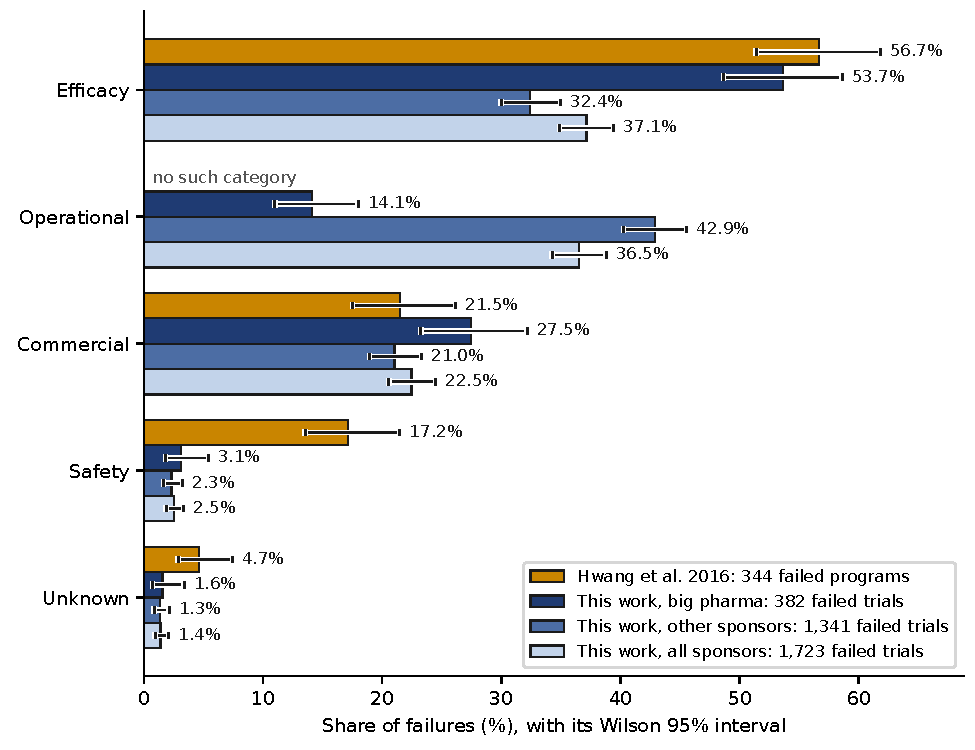
\includegraphics[width=\textwidth]{figures/ph3_failure_2016_vs_2026.pdf}
\caption{Causes of failure in Hwang et al., whose programs entered pivotal trials in \num{lit.hwang.firstYear}--\num{lit.hwang.lastYear}, and in this work, for the big-pharma stratum, for other sponsors and for all sponsors, among trials that enrolled and started in \era. Shares are of failed programs for Hwang et al.\ and of failed trials for this work. Each carries its Wilson 95\% interval, which treats the programs or the trials as independent; Figure~\ref{fig:hwang} gives the program-clustered interval of the big-pharma efficacy share. Hwang et al.\ report no operational category; their \num{hwang.other.n} failures with none of the three stated reasons are drawn as unknown. In this work, stops attributed to an undisclosed sponsor decision are counted as commercial.}
\label{fig:main}
\end{figure}

\subsection{How often a termination reason can be recovered}\label{sec:recover}
Of the \num{recover.enrolled.era.final.n} stopped trials that enrolled, started in \era\ and were not stopped for benefit, the \code{whyStopped} string alone left \num{recover.enrolled.era.first.noReason.pct}\% without a reason. After the second pass \num{recover.enrolled.era.second.unclear.pct}\% were unclear, and after the third \num{recover.enrolled.era.final.unclear.pct}\%. A further \num{recover.enrolled.era.final.sponsorundisclosed} carried the label sponsor-undisclosed, which records that the sponsor stopped the trial but not why. Counting only labels that state a reason, a reason was available for \num{recover.enrolled.era.final.reason.pct}\% of these trials, and for \num{recover.enrolled.all.final.reason.pct}\% over all years. Counting every label other than unclear as a reason, which adds sponsor-undisclosed and not-started, gives \num{recover.enrolled.era.final.notUnclear.pct}\% and \num{recover.enrolled.all.final.notUnclear.pct}\%. With withdrawn registrations included, the figures for \era\ are \num{recover.registered.era.final.reason.pct}\% and \num{recover.registered.era.final.notUnclear.pct}\%. Razuvayevskaya et al.\ assigned a reason to \num{lit.razuv.classified.pct}\% of stopped trials \cite{razuv2024}; the two figures are not like for like, because phases, years and taxonomy differ.

\subsection{The decomposition depends on which registrations are counted}\label{sec:population}
Among trials that enrolled and started in \era\ there were \num{decomp.enrolled.era.all.n} failures. Efficacy accounted for \num{decomp.enrolled.era.all.eff.pct}\% (95\% CI \num{decomp.enrolled.era.all.eff.lo} to \num{decomp.enrolled.era.all.eff.hi}), operational causes for \num{decomp.enrolled.era.all.op.pct}\% (\num{decomp.enrolled.era.all.op.lo} to \num{decomp.enrolled.era.all.op.hi}), commercial reasons for \num{decomp.enrolled.era.all.com.pct}\% (\num{decomp.enrolled.era.all.com.lo} to \num{decomp.enrolled.era.all.com.hi}), safety for \num{decomp.enrolled.era.all.saf.pct}\% (\num{decomp.enrolled.era.all.saf.lo} to \num{decomp.enrolled.era.all.saf.hi}) and unknown reasons for \num{decomp.enrolled.era.all.unk.pct}\% (\num{decomp.enrolled.era.all.unk.lo} to \num{decomp.enrolled.era.all.unk.hi}) (Figure~\ref{fig:main}; Table~\ref{tab:decomposition}). Completed trials that missed their primary endpoint made up \num{decomp.enrolled.era.all.completedMissOfEff.pct}\% of the efficacy bucket, and stops for futility the rest. The \eracomplete\ window gave efficacy \num{decomp.enrolled.complete.all.eff.pct}\% and operational \num{decomp.enrolled.complete.all.op.pct}\%; all years gave \num{decomp.enrolled.all.all.eff.pct}\% and \num{decomp.enrolled.all.all.op.pct}\%. Efficacy and operational causes are thus close in the observed data: efficacy is slightly ahead in every window, and in the main window the two intervals overlap. Over all years the unknown share is larger (\num{decomp.enrolled.all.all.unk.pct}\% against \num{decomp.enrolled.era.all.unk.pct}\%), because more of the older stops remain without a recoverable reason (\S\ref{sec:recover}).

Withdrawn registrations change this picture. They are \num{cohort.era.withdrawn.pct}\% of the stopped registrations that started in \era, and they rarely stop for efficacy: operational causes account for \num{withdrawn.era.op.pct}\% of them, the commercial bucket for \num{withdrawn.era.com.pct}\% (\num{withdrawn.era.notStated.n} of these registrations are labeled not-started or sponsor-undisclosed and state no reason) and efficacy for \num{withdrawn.era.eff.pct}\% (\num{withdrawn.era.eff.n} registrations). Counted as failures, they bring the denominator to \num{decomp.registered.era.all.n} and the shares to operational \num{decomp.registered.era.all.op.pct}\%, commercial \num{decomp.registered.era.all.com.pct}\% and efficacy \num{decomp.registered.era.all.eff.pct}\%, so that operational causes appear to outrank efficacy by a wide margin (Table~\ref{tab:decomposition}; Figure~\ref{fig:coverage}B, gray markers). Hwang et al.\ counted drugs that entered pivotal trials. A registration that never enrolled a participant is closer to a trial that was planned than to one that failed, and it is excluded from the primary analysis.

\begin{table}[htb]
\centering
% the caption stands above the table: keep it clear of the top rule
\setlength{\belowcaptionskip}{4pt}
\caption{Causes of failure by sponsor class, population and window. Shares are percentages of the failures in each row. The first row of each block is the primary analysis: trials that enrolled and started in \era; Figure~\ref{fig:main} draws its Wilson 95\% intervals. The next two rows change the window, and the fourth adds the registrations withdrawn before enrollment. In the last row, misses are imputed for unreported completed trials with a comparator arm at the miss rate of the reporting ones (\S\ref{sec:coverage}); the number after the plus sign is the misses added, and each block is imputed at its own rate. Hwang et al.\ classified programs that entered pivotal trials in \num{lit.hwang.firstYear}--\num{lit.hwang.lastYear} and report no operational category; their failures with none of the three stated reasons are given as unknown.}
\label{tab:decomposition}
\footnotesize\setlength{\tabcolsep}{5pt}
\begin{tabular}{lrrrrrr}
\toprule
population and window & failures & efficacy & operational & commercial & safety & unknown \\
\midrule
\multicolumn{7}{l}{\textit{All sponsors}} \\
enrolled, \era & \num{decomp.enrolled.era.all.n} & \num{decomp.enrolled.era.all.eff.pct} & \num{decomp.enrolled.era.all.op.pct} & \num{decomp.enrolled.era.all.com.pct} & \num{decomp.enrolled.era.all.saf.pct} & \num{decomp.enrolled.era.all.unk.pct} \\
enrolled, \eracomplete & \num{decomp.enrolled.complete.all.n} & \num{decomp.enrolled.complete.all.eff.pct} & \num{decomp.enrolled.complete.all.op.pct} & \num{decomp.enrolled.complete.all.com.pct} & \num{decomp.enrolled.complete.all.saf.pct} & \num{decomp.enrolled.complete.all.unk.pct} \\
enrolled, all years & \num{decomp.enrolled.all.all.n} & \num{decomp.enrolled.all.all.eff.pct} & \num{decomp.enrolled.all.all.op.pct} & \num{decomp.enrolled.all.all.com.pct} & \num{decomp.enrolled.all.all.saf.pct} & \num{decomp.enrolled.all.all.unk.pct} \\
withdrawn counted, \era & \num{decomp.registered.era.all.n} & \num{decomp.registered.era.all.eff.pct} & \num{decomp.registered.era.all.op.pct} & \num{decomp.registered.era.all.com.pct} & \num{decomp.registered.era.all.saf.pct} & \num{decomp.registered.era.all.unk.pct} \\
enrolled, \era, misses imputed & \num{decomp.enrolled.era.all.n} $+$ \num{coverage.enrolled.all.pooled.extra} & \num{coverage.enrolled.all.pooled.eff} & \num{coverage.enrolled.all.pooled.op} & \num{coverage.enrolled.all.pooled.com} & \num{coverage.enrolled.all.pooled.saf} & \num{coverage.enrolled.all.pooled.unk} \\
\addlinespace
\multicolumn{7}{l}{\textit{Big pharma}} \\
enrolled, \era & \num{decomp.enrolled.era.big.n} & \num{decomp.enrolled.era.big.eff.pct} & \num{decomp.enrolled.era.big.op.pct} & \num{decomp.enrolled.era.big.com.pct} & \num{decomp.enrolled.era.big.saf.pct} & \num{decomp.enrolled.era.big.unk.pct} \\
enrolled, \eracomplete & \num{decomp.enrolled.complete.big.n} & \num{decomp.enrolled.complete.big.eff.pct} & \num{decomp.enrolled.complete.big.op.pct} & \num{decomp.enrolled.complete.big.com.pct} & \num{decomp.enrolled.complete.big.saf.pct} & \num{decomp.enrolled.complete.big.unk.pct} \\
enrolled, all years & \num{decomp.enrolled.all.big.n} & \num{decomp.enrolled.all.big.eff.pct} & \num{decomp.enrolled.all.big.op.pct} & \num{decomp.enrolled.all.big.com.pct} & \num{decomp.enrolled.all.big.saf.pct} & \num{decomp.enrolled.all.big.unk.pct} \\
withdrawn counted, \era & \num{decomp.registered.era.big.n} & \num{decomp.registered.era.big.eff.pct} & \num{decomp.registered.era.big.op.pct} & \num{decomp.registered.era.big.com.pct} & \num{decomp.registered.era.big.saf.pct} & \num{decomp.registered.era.big.unk.pct} \\
enrolled, \era, misses imputed & \num{decomp.enrolled.era.big.n} $+$ \num{coverage.enrolled.big.pooled.extra} & \num{coverage.enrolled.big.pooled.eff} & \num{coverage.enrolled.big.pooled.op} & \num{coverage.enrolled.big.pooled.com} & \num{coverage.enrolled.big.pooled.saf} & \num{coverage.enrolled.big.pooled.unk} \\
\addlinespace
\multicolumn{7}{l}{\textit{Other sponsors}} \\
enrolled, \era & \num{decomp.enrolled.era.rest.n} & \num{decomp.enrolled.era.rest.eff.pct} & \num{decomp.enrolled.era.rest.op.pct} & \num{decomp.enrolled.era.rest.com.pct} & \num{decomp.enrolled.era.rest.saf.pct} & \num{decomp.enrolled.era.rest.unk.pct} \\
enrolled, \eracomplete & \num{decomp.enrolled.complete.rest.n} & \num{decomp.enrolled.complete.rest.eff.pct} & \num{decomp.enrolled.complete.rest.op.pct} & \num{decomp.enrolled.complete.rest.com.pct} & \num{decomp.enrolled.complete.rest.saf.pct} & \num{decomp.enrolled.complete.rest.unk.pct} \\
enrolled, all years & \num{decomp.enrolled.all.rest.n} & \num{decomp.enrolled.all.rest.eff.pct} & \num{decomp.enrolled.all.rest.op.pct} & \num{decomp.enrolled.all.rest.com.pct} & \num{decomp.enrolled.all.rest.saf.pct} & \num{decomp.enrolled.all.rest.unk.pct} \\
withdrawn counted, \era & \num{decomp.registered.era.rest.n} & \num{decomp.registered.era.rest.eff.pct} & \num{decomp.registered.era.rest.op.pct} & \num{decomp.registered.era.rest.com.pct} & \num{decomp.registered.era.rest.saf.pct} & \num{decomp.registered.era.rest.unk.pct} \\
enrolled, \era, misses imputed & \num{decomp.enrolled.era.rest.n} $+$ \num{coverage.enrolled.rest.pooled.extra} & \num{coverage.enrolled.rest.pooled.eff} & \num{coverage.enrolled.rest.pooled.op} & \num{coverage.enrolled.rest.pooled.com} & \num{coverage.enrolled.rest.pooled.saf} & \num{coverage.enrolled.rest.pooled.unk} \\
\addlinespace
\multicolumn{7}{l}{\textit{Hwang et al.}} \\
failed programs & \num{hwang.failed} & \num{hwang.eff.pct} & --- & \num{hwang.com.pct} & \num{hwang.saf.pct} & \num{hwang.other.pct} \\
\bottomrule
\end{tabular}
\end{table}

\subsection{Endpoint reporting under-fills the efficacy bucket}\label{sec:coverage}
Of \num{coverage.enrolled.all.completed} completed, non-stopped trials with posted results that started in \era, \num{coverage.enrolled.all.reported.n} (\num{coverage.enrolled.all.reported.pct}\%) had a verdict. Dechartres et al.\ found a similar share among completed phase 3 and phase 4 randomized superiority trials with posted results: \num{lit.dechartres.reported.pct.int}\% posted a treatment effect or $p$-value, and \num{lit.dechartres.reported.significant.pct.int}\% of those were significant. Among the others, only \num{lit.dechartres.calculated.significant.pct.int}\% were significant when the test could be computed from the posted data, which suggests selective posting of significant results \cite{dechartres2016}. In our cohort a verdict was more likely for big-pharma sponsors (odds ratio \num{covmodel.bigPharma.or}, 95\% CI \num{covmodel.bigPharma.lo} to \num{covmodel.bigPharma.hi}, $p=\num{covmodel.bigPharma.p}$), in line with the higher disclosure rates of large companies \cite{zwierzyna2018}. It became less likely with each later start year (odds ratio \num{covmodel.year.or}) and with more primary outcomes, and was much less likely for single-arm studies (odds ratio \num{covmodel.singleArm.or}, \num{covmodel.singleArm.lo} to \num{covmodel.singleArm.hi}) (supplement, Table~\ref{tab:covmodel}). Single-arm studies were \num{coverage.enrolled.all.singleArm.unreported.pct}\% of the trials without a verdict and \num{coverage.enrolled.all.singleArm.reported.pct}\% of those with one.

Stopped trials enter the decomposition whether or not they report a $p$-value. Completed trials enter it only through a reported miss. The efficacy bucket is therefore under-filled relative to the others. Among trials with a comparator arm, \num{coverage.enrolled.all.comparator.reported} had a verdict and \num{coverage.enrolled.all.comparator.unreported} did not, and \num{coverage.enrolled.all.comparator.miss.pct}\% of the former missed. Applying that rate to the latter adds about \num{coverage.enrolled.all.pooled.extra} misses and gives an efficacy share of \num{coverage.enrolled.all.pooled.eff}\% and an operational share of \num{coverage.enrolled.all.pooled.op}\% (Table~\ref{tab:decomposition}, last row of each block; the other imputations are in the supplement, Table~\ref{tab:coverage}). The sampling error of the miss rate moves the efficacy share only between \num{coverage.enrolled.all.pooled.eff.lo}\% and \num{coverage.enrolled.all.pooled.eff.hi}\%; the larger uncertainty is in the assumptions. The covariate-adjusted imputation gives \num{coverage.enrolled.all.adjusted.eff}\% and \num{coverage.enrolled.all.adjusted.op}\%. If every unreported trial with a comparator arm had missed, efficacy would be \num{coverage.enrolled.all.upper.eff}\% (Figure~\ref{fig:coverage}A). Imputing for single-arm studies as well would give \num{coverage.enrolled.all.withSingleArm.eff}\%.

Because unposted tests are significant less often than posted ones \cite{dechartres2016}, the imputed shares are likely to be too low. Because some comparator-arm trials have no between-group primary test (dose groups, cohorts, treatment sequences; \S\ref{sec:limitations}, limitation~\ref{lim:imputation}), the imputed shares may also be too high. The net direction is uncertain, and the size of the correction rests on which unreported trials are assumed able to miss. The two choices interact. With withdrawn registrations counted as failures, the same imputation gives efficacy \num{coverage.registered.all.pooled.eff}\% and operational \num{coverage.registered.all.pooled.op}\%, a tie (Figure~\ref{fig:coverage}B).

\begin{figure}[htbp]
\centering
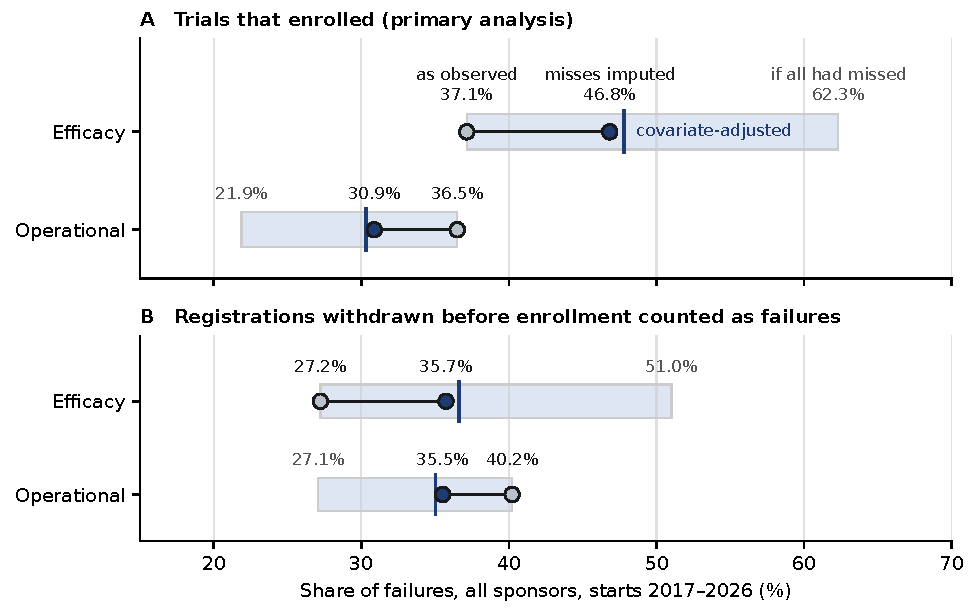
\includegraphics[width=\textwidth]{figures/ph3_coverage_correction.pdf}
\caption{The efficacy and operational shares of failures, all sponsors, starts \era, (A) among trials that enrolled and (B) with registrations withdrawn before enrollment counted as failures. Gray markers are the shares as observed. Navy markers are the shares after imputing misses for unreported completed trials with a comparator arm at the miss rate of the reporting ones, and the tick beside each is the covariate-adjusted imputation. The pale band runs from the observed share to the share if every such trial had missed; it is the range of an assumption, not a confidence interval. In B the imputed efficacy and operational shares are level.}
\label{fig:coverage}
\end{figure}

\subsection{The big-pharma efficacy share against that of Hwang et al.}\label{sec:hwang}
In the big-pharma stratum there were \num{hwang.enrolled.n} failures among trials that enrolled and started in \era, \num{decomp.enrolled.era.big.completedMiss} of them completed misses (that the total equals the number of completed misses among all sponsors in Figure~\ref{fig:flow} is a coincidence). Efficacy accounted for \num{hwang.enrolled.eff.pct}\% (Wilson 95\% CI \num{decomp.enrolled.era.big.eff.lo} to \num{decomp.enrolled.era.big.eff.hi}; program-clustered \num{hwang.enrolled.clustered.lo} to \num{hwang.enrolled.clustered.hi}, \num{hwang.enrolled.clusters} clusters), commercial reasons for \num{decomp.enrolled.era.big.com.pct}\%, operational causes for \num{decomp.enrolled.era.big.op.pct}\%, safety for \num{decomp.enrolled.era.big.saf.pct}\% and unknown reasons for \num{decomp.enrolled.era.big.unk.pct}\% (Table~\ref{tab:decomposition}). Hwang et al.\ attributed \num{hwang.eff.pct}\% (\num{hwang.eff.lo} to \num{hwang.eff.hi}) of \num{hwang.failed} failures to efficacy. The difference is not significant (two-sample $p=\num{hwang.enrolled.p}$; with program-clustered standard errors $p=\num{hwang.enrolled.clustered.p}$). The clustered 95\% interval for the difference, this work minus theirs, runs from $\num{hwang.enrolled.diff.lo}$ to $\num{hwang.enrolled.diff.hi}$ percentage points, so the data do not exclude a difference of several points in either direction. With \num{bigpharma.mid} mid-size companies added to the stratum the share is lower, \num{hwang.wide.eff.pct}\% of \num{hwang.wide.n} failures (clustered $p=\num{hwang.wide.clustered.p}$; difference $\num{hwang.wide.diff.lo}$ to $\num{hwang.wide.diff.hi}$ points), which is compatible with no difference and with a share well below theirs. In the \eracomplete\ window the share is \num{hwang.complete.eff.pct}\% (clustered $p=\num{hwang.complete.clustered.p}$; supplement, Table~\ref{tab:hwang}).

This result depends on the population. With withdrawn registrations counted, the big-pharma efficacy share falls to \num{hwang.registered.eff.pct}\%, lower than that of Hwang et al.\ (difference $\num{hwang.registered.diff.lo}$ to $\num{hwang.registered.diff.hi}$ percentage points; $p=\num{hwang.registered.p}$; clustered $p=\num{hwang.registered.clustered.p}$). Among trials that enrolled, imputing unreported misses as in \S\ref{sec:coverage} would raise the share to \num{coverage.enrolled.big.pooled.eff}\%, above their estimate. Unreported completed trials can only add efficacy failures, so they cannot lower the observed share, whatever the error of the imputation, whose direction is uncertain (\S\ref{sec:coverage}). The closeness of the observed share to their estimate is therefore not evidence of agreement. What the data support is the direction when withdrawn registrations are counted (lower) and the width of the clustered intervals of the difference (Figure~\ref{fig:hwang}; supplement, Table~\ref{tab:hwang}). Hwang et al.\ followed each drug program for years after its pivotal trials and classified the failed ones from several sources, so neither our observed share nor our imputed share is the exact counterpart of theirs.

\begin{figure}[htbp]
\centering
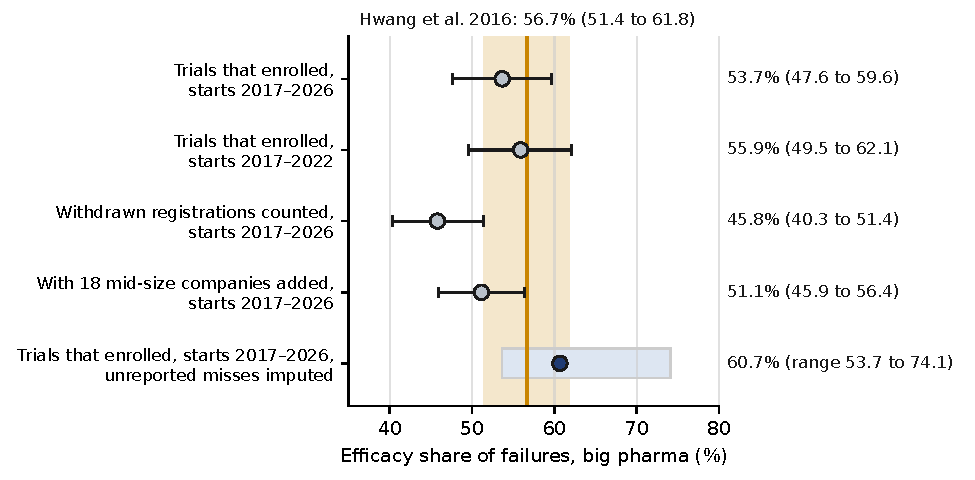
\includegraphics[width=\textwidth]{figures/ph3_bigpharma_vs_hwang.pdf}
\caption{The efficacy share of failures in the big-pharma stratum under each counting choice, against the estimate of Hwang et al.\ (ochre line, with its Wilson 95\% interval as a band). Gray markers are observed shares with their program-clustered 95\% intervals: among trials that enrolled in the main window, among those of the window that has read out, with registrations withdrawn before enrollment counted as failures, and with \num{bigpharma.mid} mid-size companies added to the stratum. The navy marker is the share after imputing misses for unreported completed trials with a comparator arm. It has no such interval; the pale band is the range from none of those trials having missed, which is the observed share, to all of them. The numbers at the right are the shares with their intervals or range.}
\label{fig:hwang}
\end{figure}

The comparison is by proxy in another respect. Hwang et al.\ studied novel therapeutics. Restricting the big-pharma stratum to trials whose subject drug had no earlier phase-3 win in the cohort left \num{novelty.novel.n} failures, of which efficacy accounted for \num{novelty.novel.eff.pct}\% (Wilson 95\% CI \num{novelty.novel.eff.lo} to \num{novelty.novel.eff.hi}). That share is lower than theirs, though not significantly (difference $\num{novelty.novel.hwang.diff.lo}$ to $\num{novelty.novel.hwang.diff.hi}$ percentage points, $p=\num{novelty.novel.hwang.p}$, trials treated as independent; clustering by program would widen the interval). This subset is the closest counterpart of their cohort. As an estimate for novel drugs its share is in this respect if anything too high: the flag sees only wins inside the cohort, so the novel group still contains lifecycle trials, and among the \num{novelty.lifecycle.n} failures of the trials flagged lifecycle, efficacy accounted for \num{novelty.lifecycle.eff.pct}\% (supplement, Table~\ref{tab:novelty}). The two subsets missed their primary endpoint equally often (\num{novelty.novel.miss.pct}\% and \num{novelty.lifecycle.miss.pct}\% of trials with a verdict). The efficacy shares differ because commercial stops are \num{novelty.novel.com.pct}\% of the failures of the novel subset and \num{novelty.lifecycle.com.pct}\% of those of the lifecycle subset, and a commercial stop can follow disappointing data.

\subsection{Few safety failures are recorded, and the taxonomy matters}\label{sec:safety}
Safety accounted for \num{decomp.enrolled.era.all.saf.pct}\% of failures among all sponsors and \num{decomp.enrolled.era.big.saf.pct}\% in the big-pharma stratum, against \num{hwang.saf.pct}\% in Hwang et al., about \num{hwang.safetyFold.big} to \num{hwang.safetyFold.all} times lower. Razuvayevskaya et al.\ found a similarly small share in stopped trials of all phases, \num{lit.razuv.safety.pct}\% of which were classified as stopped for safety or side effects \cite{razuv2024}; that share, too, is read from stated stop reasons. We cannot say how much of the gap reflects safety decisions documented outside the fields we read, how much reflects the different unit (a drug program against a trial), and how much the different period; the registry's adverse-event module was not examined. A safety-driven decision can be registered as a sponsor, business or strategic decision, and a program ended for safety after a completed trial, or at regulatory review, leaves no stopped trial at all, so the recorded share probably understates the share of failures that are due to safety. Two scenarios give the scale (supplement, Table~\ref{tab:taxonomy}). If every bare sponsor decision concealed a safety stop, safety would account for \num{tax.all.sponsorToSafety.saf}\% of failures (\num{tax.big.sponsorToSafety.saf}\% in big pharma), still below the share of Hwang et al. If every business or strategic stop did so as well, it would account for \num{tax.all.decisionsToSafety.saf}\% (\num{tax.big.decisionsToSafety.saf}\%), above it. The registry cannot show where the truth lies: it may fall below the first scenario or, if safety hides in other categories as well, above the second.

Part of the gap may be taxonomy, because stops for regulatory reasons, which we pool into operational causes, can be safety-driven. Moving half of them to safety raises the safety share to \num{tax.all.regToSafety.saf}\% for all sponsors and \num{tax.big.regToSafety.saf}\% for big pharma. Four other assignments were varied (supplement, Table~\ref{tab:taxonomy}). The adjudication of \S\ref{sec:validation} called \num{tax.external.k} of \num{tax.external.n} sampled external-evidence stops efficacy or futility; moving that share to efficacy raises the efficacy share to \num{tax.all.extToEfficacy.eff}\%. It called \num{tax.business.k} of \num{tax.business.n} sampled business or strategic stops unclear; moving that share to unknown lowers the commercial share from \num{tax.all.asAnalysed.com}\% to \num{tax.all.busToUnknown.com}\% and raises the unknown share to \num{tax.all.busToUnknown.unk}\%. Counting bare sponsor decisions as unknown lowers the commercial share to \num{tax.all.sponsorToUnknown.com}\% and raises the unknown share to \num{tax.all.sponsorToUnknown.unk}\%. Counting as unknown the \num{audit.eff.n} second-pass labels of efficacy or futility that the registry text does not support (\S\ref{sec:limitations}, limitation~\ref{lim:validation}) lowers the efficacy share to \num{tax.all.modelEfficacyToUnknown.eff}\%. None of the five changes the order of efficacy and operational causes, but the last narrows the gap to \num{tax.all.modelEfficacyToUnknown.eff}\% against \num{tax.all.modelEfficacyToUnknown.op}\%.

\subsection{Miss rate}\label{sec:missrate}
Of \num{miss.all.trials} trials with a verdict over all years (a further \num{verdict.noStartYear} have a verdict but no start date), \num{miss.all.pct}\% (95\% CI \num{miss.all.lo} to \num{miss.all.hi}) missed their primary endpoint, and \num{miss.era.pct}\% (\num{miss.era.lo} to \num{miss.era.hi}) of those starting in \era. Restricted to completed trials the rates were \num{miss.all.completed.pct}\% and \num{miss.era.completed.pct}\%.

The rate depends on the win rule (supplement, Table~\ref{tab:missrate}). The verdict counts any significant primary analysis as a win. Requiring every primary outcome that has a usable $p$-value to be significant gives \num{combine.all.and.pct}\% (\num{combine.era.and.pct}\% in \era). Requiring every primary outcome to be significant, with an outcome that has no usable $p$-value counted as not significant, gives \num{combine.all.strict.pct}\% (\num{combine.era.strict.pct}\%); \num{combine.era.incomplete.pct}\% of trials in \era\ have such an outcome. A stricter rule turns wins of completed trials into misses, which are efficacy failures: under these two rules efficacy would account for \num{winrule.and.all.eff.pct}\% and \num{winrule.strict.all.eff.pct}\% of the failures of all sponsors in the main window, against \num{winrule.and.all.op.pct}\% and \num{winrule.strict.all.op.pct}\% for operational causes, and for \num{winrule.and.big.eff.pct}\% and \num{winrule.strict.big.eff.pct}\% of big-pharma failures. Numeric readings of the minimum $p$ give \num{diag.all.naive.pct}\% with the operator stripped, \num{diag.all.sidak.pct}\% with a \v{S}id\'ak threshold on the number of primary outcomes, and \num{diag.all.single.pct}\% among trials with a single primary outcome. Excluding the \num{ni.all.pct}\% of trials that declare a non-inferiority or equivalence design, for which a $p$-value against the null is not the success criterion, changes the rate little (\num{ni.all.superiority.miss.pct}\%). Among \num{direction.wins} wins in \era, \num{direction.ratioOnly.n} (\num{direction.ratioOnly.pct}\%) had only ratio parameters above 1 among their significant analyses, \num{direction.hazardOnly.n} of them only hazard ratios above 1. The registry does not record which direction is benefit, so wins in the harmful direction cannot be counted or bounded from these fields.

Across start years \trendyears\ there was no evidence of a linear trend (Cochran--Armitage $z=\num{trend.ca.z}$, $p=\num{trend.ca.p}$; odds ratio per year \num{trend.or}, 95\% CI \num{trend.or.lo} to \num{trend.or.hi}, sponsor-clustered). Yearly rates ranged from \num{trend.max.pct}\% in \num{trend.max.year} to \num{trend.min.pct}\% in \num{trend.min.year} and stood at \num{trend.last.pct}\% in \num{trend.lastYear} (Figure~\ref{fig:missrate}; supplement, Table~\ref{tab:yearly}), a spread that a test of homogeneity does not distinguish from a constant rate ($p=\num{trend.het.p}$). The share of trials with a verdict also changes with start year (within the main window it falls, \S\ref{sec:coverage}), so these rates describe reporting trials. With the operator stripped the same trend test shows a decline ($p=\num{trend.naive.p}$), which disappears when the operator is honored.

\begin{figure}[htbp]
\centering
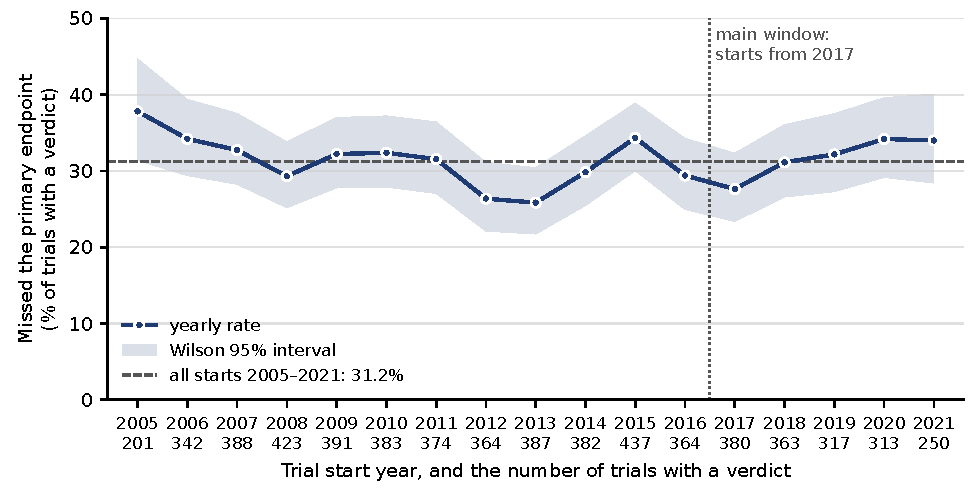
\includegraphics[width=\textwidth]{figures/ph3_miss_rate_by_year.pdf}
\caption{Share of trials with a verdict that missed their primary endpoint, by start year, with its Wilson 95\% interval (band). The number under each year is the number of trials with a verdict. The dashed line is the rate over all starts of \trendyears\ (\num{trend.overall.pct}\%). The yearly rates show no linear trend (Cochran--Armitage $p=\num{trend.ca.p}$), and a test of homogeneity does not distinguish them from a constant rate ($p=\num{trend.het.p}$). They describe the trials that report a usable primary $p$-value, a share that falls with later start years within the main window (\S\ref{sec:coverage}); start years after \num{trend.lastYear} are not drawn, because few of their trials have read out. The dotted line marks the start of \num{era.first}, the first start year of the main window of the decomposition.}
\label{fig:missrate}
\end{figure}

\subsection{Sponsor class and therapeutic area}\label{sec:sponsor}
Big-pharma trials missed their primary endpoint less often than trials of other sponsors: \num{sponsor.big.miss.pct}\% (\num{sponsor.big.miss.n} of \num{sponsor.big.trials}) against \num{sponsor.rest.miss.pct}\% (\num{sponsor.rest.miss.n} of \num{sponsor.rest.trials}; two-proportion $z=\num{sponsor.z}$, $p=\num{sponsor.p}$; program-clustered odds ratio \num{sponsor.or}, $p=\num{sponsor.or.p}$). The contrast is among trials that report a usable primary $p$-value, which big-pharma trials do more often (\S\ref{sec:coverage}). Among failures, efficacy accounted for \num{decomp.enrolled.era.big.eff.pct}\% in big pharma and \num{decomp.enrolled.era.rest.eff.pct}\% for other sponsors, whose largest bucket was operational (\num{decomp.enrolled.era.rest.op.pct}\%; Figure~\ref{fig:main}; Table~\ref{tab:decomposition}). These are shares of failures: big-pharma trials miss their endpoint less often, so a larger efficacy share does not mean more efficacy failures per trial. By therapeutic area the miss rate ranged from \num{strat.miss.min}\% (\num{strat.miss.min.area}) to \num{strat.miss.max}\% (\num{strat.miss.max.area}) ($\chi^2=\num{area.het.chi2}$, \num{area.het.dof} degrees of freedom, $p=\num{area.het.p}$; supplement, Table~\ref{tab:areas}). The cross-sectional design cannot separate sponsor class from target maturity, trial size or therapeutic area.

\subsection{Validation}\label{sec:validation}
The first-pass label agreed with the blind adjudication for \num{valid.agree.n} of \num{valid.sample} sampled items (\num{valid.agree.pct}\%, 95\% CI \num{valid.agree.lo} to \num{valid.agree.hi}; Cohen's $\kappa=\num{valid.kappa}$). Weighted to the prevalence of the first-pass labels, agreement was \num{valid.weighted.pct}\% (bootstrap 95\% CI \num{valid.weighted.lo} to \num{valid.weighted.hi}; $\kappa=\num{valid.weighted.kappa}$). Weighted to the labels of trials that enrolled and started in \era, it was \num{valid.weightedEra.pct}\% (\num{valid.weightedEra.lo} to \num{valid.weightedEra.hi}). Agreement was complete for funding and \mbox{COVID-19} (\num{valid.cat.funding.agree} of \num{valid.perCategory} each) and lowest for external evidence (\num{valid.cat.externalevidence.agree} of \num{valid.perCategory}; where the adjudication differed, most often as efficacy or futility) and for business or strategic (\num{valid.cat.businessstrategic.agree} of \num{valid.perCategory}; most often as unclear) (supplement, Table~\ref{tab:validation}). The per-category samples are small and their intervals wide. A disagreement between two categories of the same bucket does not move a share of the decomposition: the two labels fell in the same bucket for \num{valid.bucket.agree.n} of the \num{valid.sample} items (\num{valid.bucket.agree.pct}\%, 95\% CI \num{valid.bucket.agree.lo} to \num{valid.bucket.agree.hi}), and for \num{valid.bucket.weighted.pct}\% when weighted to label prevalence. The second and third passes and the rules were not validated. They handled the trials whose first-pass label was blank or unclear, which are \num{valid.era.laterPass.pct}\% of the \num{valid.era.stopped} stopped trials that enrolled and started in \era; that count includes the stops for benefit, which \S\ref{sec:recover} leaves out.

The $p$-value extraction was not compared with source documents. The second retrieval returned the same minimum $p$ as the first for all \num{stability.compared} trials that had one in both, and the same number of primary outcomes for \num{stability.sameCount.pct}\% of trials, so the registry values are stable. Both retrievals use the same parsing code, so this does not test the parser.

\section{Discussion}\label{sec:discussion}
A registry-only decomposition of phase-3 failure is sensitive to two choices that are easy to make without noticing. The first is the population. Of the stopped registrations of the main window, \num{cohort.era.withdrawn.pct.int}\% never enrolled a participant. They stop for business reasons, funding or logistics, and counting them as failed trials lowers the efficacy share markedly, from \num{decomp.enrolled.era.all.eff.pct}\% to \num{decomp.registered.era.all.eff.pct}\%, and puts operational causes first. The second is the treatment of completed trials that report no usable primary $p$-value. They are \num{coverage.enrolled.all.unreported.pct.int}\% of completed trials with posted results, they cannot enter the efficacy bucket, and those that could have missed are numerous enough to move the efficacy share by a similar amount in the other direction, to \num{coverage.enrolled.all.pooled.eff}\% under the imputation. Neither choice is visible in the output of a decomposition, and the naive reading of each, counting every withdrawn registration and ignoring the trials without a $p$-value, makes efficacy look smaller.

With registrations that never enrolled set aside, efficacy is the leading cause of failure in the big-pharma stratum. Its observed share is not distinguishable from the manual estimate of Hwang et al., which was published a decade earlier and describes programs that entered pivotal trials in \num{lit.hwang.firstYear}--\num{lit.hwang.lastYear}. The comparison is by proxy and does not establish agreement: the interval of the difference is wide, and the share is lower, though not significantly, among trials of drugs with no earlier phase-3 win, the closer counterpart of their cohort, and when mid-size companies are added (\S\ref{sec:hwang}). These are shares of failures, not failure rates: big-pharma trials missed their primary endpoint less often than trials of other sponsors, and fewer of their failures were operational. For all sponsors efficacy is only slightly ahead of operational causes as observed, and further ahead under an imputation or under a stricter win rule, each of which rests on assumptions (\S\ref{sec:limitations}, limitations~\ref{lim:imputation} and~\ref{lim:winrule}). Safety is the exception. The registry fields we read record it \num{hwang.safetyFold.big} to \num{hwang.safetyFold.all} times less often than Hwang et al.\ did. Safety-driven stops can be registered as sponsor or business decisions, so the recorded share probably understates safety failure, and the registry cannot show by how much, or whether safety failure has become rarer.

Jovanovic et al.\ showed that methodological choices, chiefly whether ongoing trials count as non-failures and which study types are included, explain part of the variation between published failure proportions \cite{jovanovic2026}. Our results concern the causes of failure rather than its proportion, and add two specific choices: registrations withdrawn before enrollment, and endpoint-reporting coverage with its dependence on trial design. Both can be checked in a registry-based study from fields the registry provides. Our definition departs from the one they recommend, which counts terminated and withdrawn studies as failed and completed ones as not failed; they also question the counting of suspended trials. Their failure is a trial that does not run to completion. Ours adds completed trials that missed their primary endpoint, because the comparison is with drugs that failed, and for the same reason sets aside registrations that never enrolled. The analysis with withdrawn registrations counted (\S\ref{sec:population}) is the closest to their definition. Suspended trials are counted as failures here (\S\ref{sec:limitations}).

Over all start years, \num{miss.all.pct.int}\% of phase-3 trials with a usable primary $p$-value miss their primary endpoint under the most lenient win rule and \num{combine.all.and.pct.int}\% when every primary outcome with a usable $p$-value must be significant (\num{combine.all.strict.pct.int}\% if outcomes without one count as misses). We found no evidence of a linear trend in that rate, and a test of homogeneity does not distinguish the yearly rates from a constant one. The rate describes only the trials that report.

These results describe phase-3 registrations at ClinicalTrials.gov that posted results or stopped early. They do not extend to earlier phases, to trials registered only elsewhere, or to completed trials that never posted results.

\section{Limitations}\label{sec:limitations}
\begin{enumerate}[leftmargin=*]
\item\label{lim:coverage} \textbf{The cohort excludes completed trials that never posted results.} In one audit, results had been submitted for \num{lit.devito.submitted.pct.int}\% of the trials due to report \cite{devito2020}, and dissemination rates vary widely between academic medical centers \cite{chen2016}. The imputation of \S\ref{sec:coverage} covers completed trials with posted results only, and its bounds are conditional on the cohort.
\item\label{lim:imputation} \textbf{The imputation rests on assumptions.} It treats every unreported trial with a comparator arm as able to miss and every single-arm study as unable to, and it models the miss probability from four covariates. Two or more arm groups do not guarantee a between-group primary test: dose groups, cohorts and treatment sequences are arm groups too, and the allocation and the intervention model were not retrieved. Reporting is not random, so the imputed shares indicate direction and rough size, not a corrected estimate.
\item\label{lim:population} \textbf{The population is defined by registry status.} Setting withdrawn registrations aside is one of the two choices that matter most here: counting them moves the efficacy share from \num{decomp.enrolled.era.all.eff.pct}\% to \num{decomp.registered.era.all.eff.pct}\% (\S\ref{sec:population}). They are excluded on the registry's definition of that status; enrollment counts were not used to define the population, so a terminated or suspended registration counts as enrolled whatever its recorded enrollment. Suspended trials (\num{cohort.suspended} in the cohort) are counted as failures although some may resume. Registrations designated Phase 2/Phase~3 are kept and cannot be told apart, and \num{cohort.noDrug.pct}\% of registrations test no drug or biological product (\S\ref{sec:data}).
\item\label{lim:pvalue} \textbf{The $p$-value extraction was not checked against source documents.} Data-entry errors inside the registry are invisible to it; \num{pvalue.invalid.records} records in \num{pvalue.invalid.trials} trials carry a $p$-value outside $[0, 1]$ and were treated as missing.
\item\label{lim:winrule} \textbf{The primary verdict is lenient.} Any significant primary analysis scores a win, including one of several analyses of the same outcome, and the direction of effect is not recorded. \S\ref{sec:missrate} shows how far stricter rules move the miss rate and, with it, the decomposition: under the two stricter rules efficacy would account for \num{winrule.and.all.eff.pct}\% and \num{winrule.strict.all.eff.pct}\% of failures instead of \num{decomp.enrolled.era.all.eff.pct}\%, so the lenient verdict works against efficacy.
\item\label{lim:hwang} \textbf{The comparison with Hwang et al.\ is by proxy.} The big-pharma stratum is defined by our list of companies and by name patterns matched on the lead sponsor only. A subsidiary or an acquired company is counted with its parent whatever the date of the trial, and a business that was later spun off is counted with its former parent, so trials that an acquired company started before its acquisition count as big-pharma trials. The stratum is narrower than their cohort, which included small and mid-size companies. Their unit is a drug program and ours a trial, their programs entered pivotal trials in \num{lit.hwang.firstYear}--\num{lit.hwang.lastYear}, and their classification had access to sources outside the registry. A trial that missed its primary endpoint counts as a failure here even if the same drug succeeded in another trial or was later approved, and a trial stopped for slow enrollment counts as one even if the program went on.
\item\label{lim:safety} \textbf{Safety is read from two free-text fields and is probably understated.} Only the \code{whyStopped} string and the detailed description were examined; the adverse-event module was not. A safety-driven decision can be registered as a sponsor, business or strategic decision, and the fields we read cannot show how often (\S\ref{sec:safety}), so the gap to Hwang et al.\ cannot be attributed.
\item\label{lim:validation} \textbf{The validation is model-based, small per category and limited to the first pass.} The adjudicator is a stronger model of the same family, so shared blind spots cannot be ruled out. Labels from the later passes and from the rules were not validated. Of the \num{audit.model.n} second-pass model labels among the stops of the main window, \num{audit.eff.n} are efficacy or futility, and a reading of them by language-model agents during the preparation of this manuscript found none supported: neither the string nor the detailed description states such a reason (\num{audit.eff.monitoring} strings name a data monitoring committee, \num{audit.eff.interim} an interim analysis and \num{audit.eff.other} a sponsor decision, none with a reason). None is a big-pharma trial. Counted as unknown, these labels would lower the efficacy share of all sponsors from \num{decomp.enrolled.era.all.eff.pct}\% to \num{tax.all.modelEfficacyToUnknown.eff}\%, against \num{tax.all.modelEfficacyToUnknown.op}\% for operational causes (\S\ref{sec:safety}; the registrations are listed in the supplement, \S\ref{supp:taxonomy}). The labels were left as the model gave them. The same reading found unsupported labels in the operational bucket as well, and the labels of other start years were not read. The model versions were not recorded, and the classification cannot be re-run from the archive.
\item\label{lim:taxonomy} \textbf{Category boundaries are contestable.} The assignments varied in \S\ref{sec:safety} move the commercial and unknown shares by several points and the safety share by less. The enrollment label that a rule gives to stops after few participants (\S\ref{sec:classification}) is inferred from the count, not stated by the sponsor; it adds only to the operational bucket, so dropping it would widen the lead of efficacy.
\item\label{lim:heuristics} \textbf{Subject drugs and therapeutic areas are assigned by heuristics.} The subject drug is the rarest experimental-arm drug, which is unreliable for combination and platform regimens, and the area comes from a keyword match on condition terms. Neither was audited trial by trial. They affect the program-clustered intervals and tests, the novelty flag and the results by therapeutic area.
\item\label{lim:censoring} \textbf{Recent starts are right-censored.} A stopped trial enters the cohort at once and a completed trial only when its results are posted, so the latest start years are short of completed misses and the efficacy share of the main window is understated. The \eracomplete\ window, where the share is higher, addresses this only in part.
\item\label{lim:unit} \textbf{The trial is the unit of analysis.} Trials of the same drug program are not independent, so intervals and tests that are not clustered by program are too narrow: for the big-pharma efficacy share the Wilson interval runs from \num{decomp.enrolled.era.big.eff.lo}\% to \num{decomp.enrolled.era.big.eff.hi}\% and the program-clustered one from \num{hwang.enrolled.clustered.lo}\% to \num{hwang.enrolled.clustered.hi}\%. The shares also weight a program by its number of failed trials, whereas Hwang et al.\ counted each program once. The test of the novel subset (\S\ref{sec:hwang}) treats trials as independent.
\item\label{lim:plan} \textbf{The analysis was not pre-specified.} No protocol was registered. The windows, the big-pharma stratum and the sensitivity analyses were defined during the work, and the stratum was narrowed to the \num{bigpharma.companies} large companies after results for a list that included mid-size companies had been seen; that wider list is reported as a sensitivity analysis (\S\ref{sec:hwang}). The $p$-values are descriptive and none is adjusted for multiplicity.
\end{enumerate}

\section{Data and code availability}\label{sec:availability}
All analysis code, the classification prompts, every label, the recorded numbers and tables, the figures and the registry retrievals of \num{retrieval.cohort} and \num{retrieval.analyses} are public at \url{https://github.com/tommycarstensen/phase3-failure-decomposition}. The ClinicalTrials.gov API returns the current version of each record, so the archived retrievals, not a fresh pull, are the data of record. \code{reproduce.sh} regenerates every number, table and figure in this paper from them and checks that the text contains no number typed by hand. The PubMed abstracts read in the third classification pass are not redistributed; \code{fetch\_pubmed.py} retrieves them by PMID.

\section{Declarations}\label{sec:declarations}
\noindent\textbf{Correspondence.} \href{mailto:tommy.carstensen@regionh.dk}{tommy.carstensen@regionh.dk} (ORCID \href{https://orcid.org/0000-0002-3672-9931}{0000-0002-3672-9931}).

\noindent\textbf{Funding.} This work received no funding.

\noindent\textbf{Competing interests.} The author declares no competing interests.

\noindent\textbf{Ethics.} The study used only publicly available registry records and published abstracts. It involved no human participants and no individual-level data, so ethics approval was not required.

\noindent\textbf{Trial registration.} Not applicable: this is an analysis of registry records, not a clinical trial.

\noindent\textbf{Use of AI tools.} Large language models are part of the method: Claude Sonnet classified the termination reasons and Claude Opus adjudicated the validation sample (\S\ref{sec:classification}, \S\ref{sec:validation-methods}). The Claude Code assistant (Anthropic) was also used to write and review the analysis code and to draft and edit this manuscript. The author reviewed the code, the results and the text, and takes full responsibility for the content.

\begin{thebibliography}{99}
\bibitem{teodoro2025} Teodoro D, Naderi N, Yazdani A, Zhang B, Bornet A. A scoping review of artificial intelligence applications in clinical trial risk assessment. \emph{npj Digit Med.} 2025;8:486.
\bibitem{williams2015} Williams RJ, Tse T, DiPiazza K, Zarin DA. Terminated trials in the ClinicalTrials.gov results database: evaluation of availability of primary outcome data and reasons for termination. \emph{PLoS ONE.} 2015;10(5):e0127242.
\bibitem{razuv2024} Razuvayevskaya O, Lopez I, Dunham I, Ochoa D. Genetic factors associated with reasons for clinical trial stoppage. \emph{Nat Genet.} 2024;56(9):1862--1867.
\bibitem{luo2023} Luo J, Qiao Z, Glass L, Xiao C, Ma F. ClinicalRisk: a new therapy-related clinical trial dataset for predicting trial status and failure reasons. \emph{Proc CIKM.} 2023:5356--5360.
\bibitem{kavalci2023} Kavalci E, Hartshorn A. Improving clinical trial design using interpretable machine learning based prediction of early trial termination. \emph{Sci Rep.} 2023;13:121.
\bibitem{gao2024} Gao C, Pradeepkumar J, Das T, Thati S, Sun J. Automatically labeling clinical trial outcomes: a large-scale benchmark for drug development. \emph{arXiv.} 2024:2406.10292.
\bibitem{jovanovic2026} Jovanovic A, Gavric S, Dennst\"adt F, Cihoric N. Approaches in analyzing predictors of trial failure: a scoping review and meta-epidemiological study. \emph{BMC Med Res Methodol.} 2026;26:35.
\bibitem{hwang2016} Hwang TJ, Carpenter D, Lauffenburger JC, Wang B, Franklin JM, Kesselheim AS. Failure of investigational drugs in late-stage clinical development and publication of trial results. \emph{JAMA Intern Med.} 2016;176(12):1826--1833.
\bibitem{fda2017} U.S. Department of Health and Human Services. Clinical Trials Registration and Results Information Submission; Final Rule. 42 CFR Part 11. \emph{Fed Regist.} 2016;81(183):64982--65157.
\bibitem{brown2001} Brown LD, Cai TT, DasGupta A. Interval estimation for a binomial proportion. \emph{Statist Sci.} 2001;16(2):101--133.
\bibitem{cohen1960} Cohen J. A coefficient of agreement for nominal scales. \emph{Educ Psychol Meas.} 1960;20(1):37--46.
\bibitem{cochran1954} Cochran WG. Some methods for strengthening the common $\chi^2$ tests. \emph{Biometrics.} 1954;\allowbreak \mbox{10(4):417--451}.
\bibitem{armitage1955} Armitage P. Tests for linear trends in proportions and frequencies. \emph{Biometrics.} 1955;\allowbreak \mbox{11(3):375--386}.
\bibitem{vonelm2007} von Elm E, Altman DG, Egger M, Pocock SJ, G{\o}tzsche PC, Vandenbroucke JP. The Strengthening the Reporting of Observational Studies in Epidemiology (STROBE) statement: guidelines for reporting observational studies. \emph{Lancet.} 2007;370(9596):1453--1457.
\bibitem{dechartres2016} Dechartres A, Bond EG, Scheer J, Riveros C, Atal I, Ravaud P. Reporting of statistically significant results at ClinicalTrials.gov for completed superiority randomized controlled trials. \emph{BMC Med.} 2016;14:192.
\bibitem{zwierzyna2018} Zwierzyna M, Davies M, Hingorani AD, Hunter J. Clinical trial design and dissemination: comprehensive analysis of clinicaltrials.gov and PubMed data since 2005. \emph{BMJ.} 2018;361:k2130.
\bibitem{devito2020} DeVito NJ, Bacon S, Goldacre B. Compliance with legal requirement to report clinical trial results on ClinicalTrials.gov: a cohort study. \emph{Lancet.} 2020;395(10221):361--369.
\bibitem{chen2016} Chen R, Desai NR, Ross JS, Zhang W, Chau KH, Wayda B, Murugiah K, Lu DY, Mittal A, Krumholz HM. Publication and reporting of clinical trial results: cross sectional analysis across academic medical centers. \emph{BMJ.} 2016;352:i637.
\end{thebibliography}

\end{document}
